% ============================================================
% Rapport du projet – Ossatures de bâtiments
% CHEBAP/TS – Fatoumata Bineta SALL – 2025-2026
% Chargé de TD : M. Bodet
% ============================================================
%
% Document principal : ce fichier sert d'orchestrateur.
% Tout le contenu est réparti dans :
%   - preambule.tex                       : packages et commandes
%   - meta/page-de-garde.tex              : page de titre
%   - meta/enonce.tex                     : énoncé du projet (à compléter)
%   - seances/seance-XX-*/seance-XX.tex   : contenu de chaque séance
%   - meta/synthese-resultats.tex         : synthèse finale
%
% Pour ajouter une image dans une séance :
%   1. Placer l'image dans seances/seance-XX-*/images/
%   2. Dans seance-XX.tex, remplacer \figureplaceholder{nom}{légende} par :
%        \begin{figure}[H]\centering
%          \includegraphics[width=0.7\linewidth]{nom.png}
%          \caption{légende}\label{fig:nom}
%        \end{figure}
% ============================================================

\documentclass[a4paper,11pt]{article}

% ============================================================
% Préambule LaTeX — Rapport Ossatures de bâtiments
% CHEBAP/TS – Fatoumata Bineta SALL – 2025-2026
% ============================================================

\usepackage[utf8]{inputenc}
\usepackage[T1]{fontenc}
\usepackage[french]{babel}
\usepackage[top=2.2cm,bottom=2.5cm,left=2.5cm,right=2.5cm]{geometry}

\usepackage{amsmath,amssymb,mathtools}

\usepackage[dvipsnames]{xcolor}
\definecolor{bleu}{RGB}{30,80,125}
\definecolor{gris}{RGB}{110,110,110}
% Couleurs du logo CHEBAP (échantillonnées sur l'énoncé)
\definecolor{chebaprouge}{RGB}{212,42,10}    % CHE en rouge vermillon
\definecolor{chebapgris}{RGB}{126,123,122}   % BAP en gris moyen

\usepackage{tcolorbox}
\tcbuselibrary{skins,breakable}
\usepackage{tikz}
\usepackage{float}
\usepackage{graphicx}

% Note : \graphicspath sera défini dans main.tex pour pointer vers tous les
% sous-dossiers images/ des séances.

% Pour intégrer le scan de l'énoncé en début de rapport
\usepackage{pdfpages}

% Résultat encadré
\newcommand{\encadre}[1]{%
  \begin{tcolorbox}[
    enhanced, colback=white, colframe=black,
    boxrule=0.8pt, arc=0pt, sharp corners,
    halign=center,
    left=6pt, right=6pt, top=4pt, bottom=4pt
  ]
  #1
  \end{tcolorbox}\vspace{2pt}%
}

% Espace réservé pour image — Renommer ton image en "<nom>.png" puis la mettre
% dans le dossier "images/" de la séance correspondante
\newcommand{\figureplaceholder}[2]{%
  \begin{figure}[H]
    \centering
    \fbox{\begin{minipage}[c][5cm][c]{0.7\linewidth}
      \centering
      \color{gris}\itshape\small
      \textbf{[ Image à insérer ]}\\[4pt]
      Renommer votre fichier en :\\
      \texttt{#1.png}\\[4pt]
      Légende : #2
    \end{minipage}}
    \caption{#2}
    \label{fig:#1}
  \end{figure}%
}
% Pour utiliser l'image après l'avoir mise dans le dossier images/, remplacer par :
% \begin{figure}[H]\centering
%   \includegraphics[width=0.7\linewidth]{nom_image.png}
%   \caption{...}\label{fig:nom_image}
% \end{figure}

\usepackage{setspace}
\setstretch{1.5}
\setlength{\parindent}{1.2cm}
\setlength{\parskip}{3pt}

\usepackage{booktabs,array,tabularx}
\usepackage{multirow}
\renewcommand{\arraystretch}{1.25}

\usepackage{enumitem}
\setlist[itemize]{label=---,left=0.6cm,topsep=2pt,itemsep=1pt}

\usepackage{titlesec}
\titleformat{\section}{\large\bfseries\color{bleu}}{}{0em}{}[{\color{bleu}\vspace{-4pt}\rule{\linewidth}{0.5pt}}]
\titleformat{\subsection}{\normalsize\bfseries\color{bleu}}{}{0em}{}
\titleformat{\subsubsection}{\normalsize\bfseries}{}{0em}{}
\titlespacing{\section}{0pt}{18pt}{8pt}
\titlespacing{\subsection}{0pt}{12pt}{4pt}
\titlespacing{\subsubsection}{0pt}{8pt}{3pt}

\setcounter{secnumdepth}{3}
\setcounter{tocdepth}{2}

\usepackage{hyperref}
\hypersetup{colorlinks,linkcolor=bleu,urlcolor=bleu}

% Bandeau de séance : page de garde dédiée + entrée TOC en niveau 1.
%
% Usage :
%   \seance{N}{titre}        -> sous-sections numérotées N.1, N.2, ...
%   \seance[N]{N \& M}{titre} -> idem, avec N en argument optionnel
%
% L'argument optionnel sert pour les séances groupées (« 5 \& 6 »,
% « 11 \& 12 ») où le premier argument n'est pas un nombre exploitable
% par \setcounter. Par défaut, on suppose que #1 est un entier et on
% l'utilise directement.
\newcommand{\seance}[3][]{%
  \clearpage
  \def\seancenum{\ifx\\#1\\#2\else#1\fi}%
  \setcounter{section}{\numexpr\seancenum-1\relax}%
  \refstepcounter{section}%
  \phantomsection
  \addcontentsline{toc}{section}{Séance #2 : #3}%
  \thispagestyle{empty}
  \vspace*{\fill}
  \begin{tcolorbox}[
    enhanced, colback=bleu, colframe=bleu,
    boxrule=0pt, arc=0pt, sharp corners,
    fontupper=\color{white}\Huge\bfseries,
    halign=center,
    left=20pt, right=20pt, top=30pt, bottom=30pt
  ]
  Séance #2\\[12pt]{\LARGE\mdseries #3}
  \end{tcolorbox}
  \vspace*{\fill}
  \clearpage
}

% Variante : bandeau de section spéciale (énoncé, synthèse) sans
% numéro de séance, mais avec le même style graphique. Ces sections
% n'ont pas de \subsection numérotée à l'intérieur, donc on
% n'incrémente pas le compteur de section : la numérotation des
% séances suit ainsi 1, 2, ..., 10 sans décalage.
% Usage : \sectionspeciale{Énoncé du projet}
\newcommand{\sectionspeciale}[1]{%
  \clearpage
  \phantomsection
  \addcontentsline{toc}{section}{#1}%
  \thispagestyle{empty}
  \vspace*{\fill}
  \begin{tcolorbox}[
    enhanced, colback=bleu, colframe=bleu,
    boxrule=0pt, arc=0pt, sharp corners,
    fontupper=\color{white}\Huge\bfseries,
    halign=center,
    left=20pt, right=20pt, top=30pt, bottom=30pt
  ]
  #1
  \end{tcolorbox}
  \vspace*{\fill}
  \clearpage
}


% Le \graphicspath couvre tous les sous-dossiers images/ des séances.
\graphicspath{%
  {meta/}%
  {seances/seance-01-predimensionnement/images/}%
  {seances/seance-02-descente-charges/images/}%
  {seances/seance-03-semelles/images/}%
  {seances/seance-04-dalle-4-cotes/images/}%
  {seances/seances-05-06-poutre/images/}%
  {seances/seance-07-escalier/images/}%
  {seances/seance-08-mur-pignon/images/}%
  {seances/seance-09-mur-sous-sol/images/}%
  {seances/seance-10-calcul-feu/images/}%
  {seances/seances-11-12-plancher-dalle/images/}%
}

\begin{document}

% ════════════════ PAGE DE GARDE ══════════════════════════════
% ============================================================
% Page de garde
% ============================================================

\begin{titlepage}
  \centering
  \vspace*{1.5cm}
  {\Huge\bfseries\color{chebaprouge}CHE\color{chebapgris}BAP\color{gris}/TS\par}
  \vspace{1.2cm}
  \begin{tcolorbox}[enhanced,colback=white,colframe=bleu,boxrule=1.5pt,
    arc=0pt,sharp corners,width=12cm,halign=center]
    {\Large Rapport du projet}\\[6pt]
    {\LARGE\bfseries Ossatures de bâtiments}
  \end{tcolorbox}
  \vspace{1.5cm}
  {\large Rédigé par :}\\[8pt]
  {\Large\bfseries Fatoumata Bineta SALL}\\[1.4cm]
  {\large Chargé de TD :}\\[6pt]
  {\large M.\,Bodet}\\[2cm]
  {\large Année Universitaire}\\[6pt]
  {\Large\bfseries\color{bleu} 2025 -- 2026}
  \vfill
\end{titlepage}


% ════════════════ TABLE DES MATIÈRES ═════════════════════════
\tableofcontents
\newpage

% ════════════════ TABLE DES FIGURES ══════════════════════════
\listoffigures
\newpage

% ════════════════ AVANT-PROPOS ═══════════════════════════════
% ============================================================
% Avant-propos
% Présentation des outils utilisés pour la production du rapport :
% LaTeX, GitHub et GitHub Actions.
% ============================================================

\sectionspeciale{Avant-propos}

\subsection*{Sur le choix de \LaTeX{}}

Le présent rapport est rédigé en \LaTeX{}, un système de composition de
documents largement utilisé dans le milieu universitaire et l'édition
scientifique. J'ai eu l'occasion de me familiariser avec cet outil lors
de la rédaction de mon mémoire de Master~2 en génie civil, dont les
sources sont consultables à l'adresse suivante :
\url{https://drive.google.com/drive/folders/1xuWxaYyATofsG46Qz3gQ8edoHxM41sDl?usp=drive_link}.

Le choix de \LaTeX{} pour ce rapport tient à plusieurs raisons concrètes.
D'abord, la qualité typographique des formules mathématiques et le soin
apporté à la mise en page des équations longues, qui sont nombreuses
dans un rapport de calcul de structures. Ensuite, la stabilité des
références croisées : chaque figure, chaque tableau, chaque équation
porte une étiquette interne, et leur numérotation se met à jour
automatiquement au fil des modifications, sans risque de
désynchronisation entre le texte et les renvois. Enfin, le format de
sortie est un document PDF reproductible, c'est-à-dire qu'à partir des
mêmes fichiers source, n'importe quel lecteur obtient le même PDF
identique au caractère près.

Le rapport est organisé en plusieurs fichiers source : un fichier
principal qui orchestre la compilation, un préambule contenant les
réglages de mise en page, et un fichier par séance regroupant le texte,
les calculs et les figures de la séance. Cette organisation modulaire
facilite la relecture et permet de travailler sur une séance sans
toucher aux autres.

\subsection*{Sur l'usage de GitHub}

Les fichiers source du rapport sont hébergés sur GitHub, une plateforme
publique de stockage de code et de documents textuels. L'adresse du
dépôt est :
\url{https://github.com/fatoumata-gc/ossature-batiment-chec}.

GitHub joue ici le rôle d'archive consultable et historique. Chaque
modification apportée à un fichier est enregistrée avec sa date, son
auteur et une description, ce qui permet de retrouver à tout moment
l'état du rapport à une étape antérieure du travail. Cette traçabilité
n'est pas une fin en soi : elle reflète simplement la même rigueur
qu'un cahier de laboratoire daté et paraphé. Pour un examinateur qui
souhaiterait consulter directement les sources, vérifier une formule
dans son contexte de calcul ou observer la progression du travail au
cours du semestre, l'historique du dépôt en offre la possibilité.

\subsection*{Sur GitHub Actions, et ce que ce n'est pas}

Une seule fonctionnalité de GitHub mérite ici une explication un peu
plus précise, car son nom peut prêter à confusion : il s'agit de
GitHub~Actions.

GitHub~Actions est un service d'automatisation. Concrètement, il permet
de demander au serveur d'exécuter une tâche programmée chaque fois
qu'un fichier source est modifié. Dans le cas du présent rapport, la
tâche est unique et très simple : à chaque mise à jour du dépôt, le
serveur lance la commande \texttt{pdflatex} sur le fichier
\texttt{main.tex}, recompile le document et publie le PDF résultant.
C'est exactement ce que je ferais en local avec un Makefile ou un
script shell, à la différence près que la tâche est exécutée par le
serveur de GitHub plutôt que sur ma propre machine. L'intérêt pratique
est qu'on dispose toujours d'une version PDF à jour sans devoir penser
à recompiler manuellement après chaque correction.

Il me paraît important de préciser ce que GitHub~Actions \emph{n'est
pas}, car le terme « actions » peut évoquer des fonctionnalités
beaucoup plus ambitieuses qu'il ne recouvre.

GitHub~Actions n'est pas un système d'intelligence artificielle. Il ne
génère aucun contenu, ne propose aucune formulation, ne corrige aucune
phrase, ne retouche aucune équation. Le service ne fait que rejouer une
suite d'instructions définies à l'avance dans un fichier de
configuration : récupérer les fichiers source, installer la
distribution \LaTeX{}, exécuter \texttt{pdflatex} en deux passes,
produire un PDF, et le rendre téléchargeable. C'est un déclencheur de
compilation, équivalent moderne d'un Makefile. La rédaction du rapport,
le choix des hypothèses, le déroulé des calculs et la formulation des
conclusions relèvent intégralement du travail de l'auteur.

\subsection*{Lecture du rapport}

Le rapport peut être lu indépendamment de toute considération
informatique : le PDF est un document autonome qui se suffit à
lui-même. Les éléments présentés dans cet avant-propos visent
uniquement à donner au lecteur la possibilité, s'il le souhaite, de
remonter aux sources du document, de consulter son historique, ou de
recompiler le PDF à partir du dépôt public.

\clearpage


% ════════════════ ÉNONCÉ DU PROJET ═══════════════════════════
% ============================================================
% Énoncé du projet
% ============================================================
% Lorsque tu auras le scan PDF de l'énoncé, copie-le sous
% meta/enonce.pdf puis dé-commente la ligne includepdf ci-dessous
% et supprime le bloc placeholder.
% ============================================================

\section*{Énoncé du projet}
\addcontentsline{toc}{section}{Énoncé du projet}

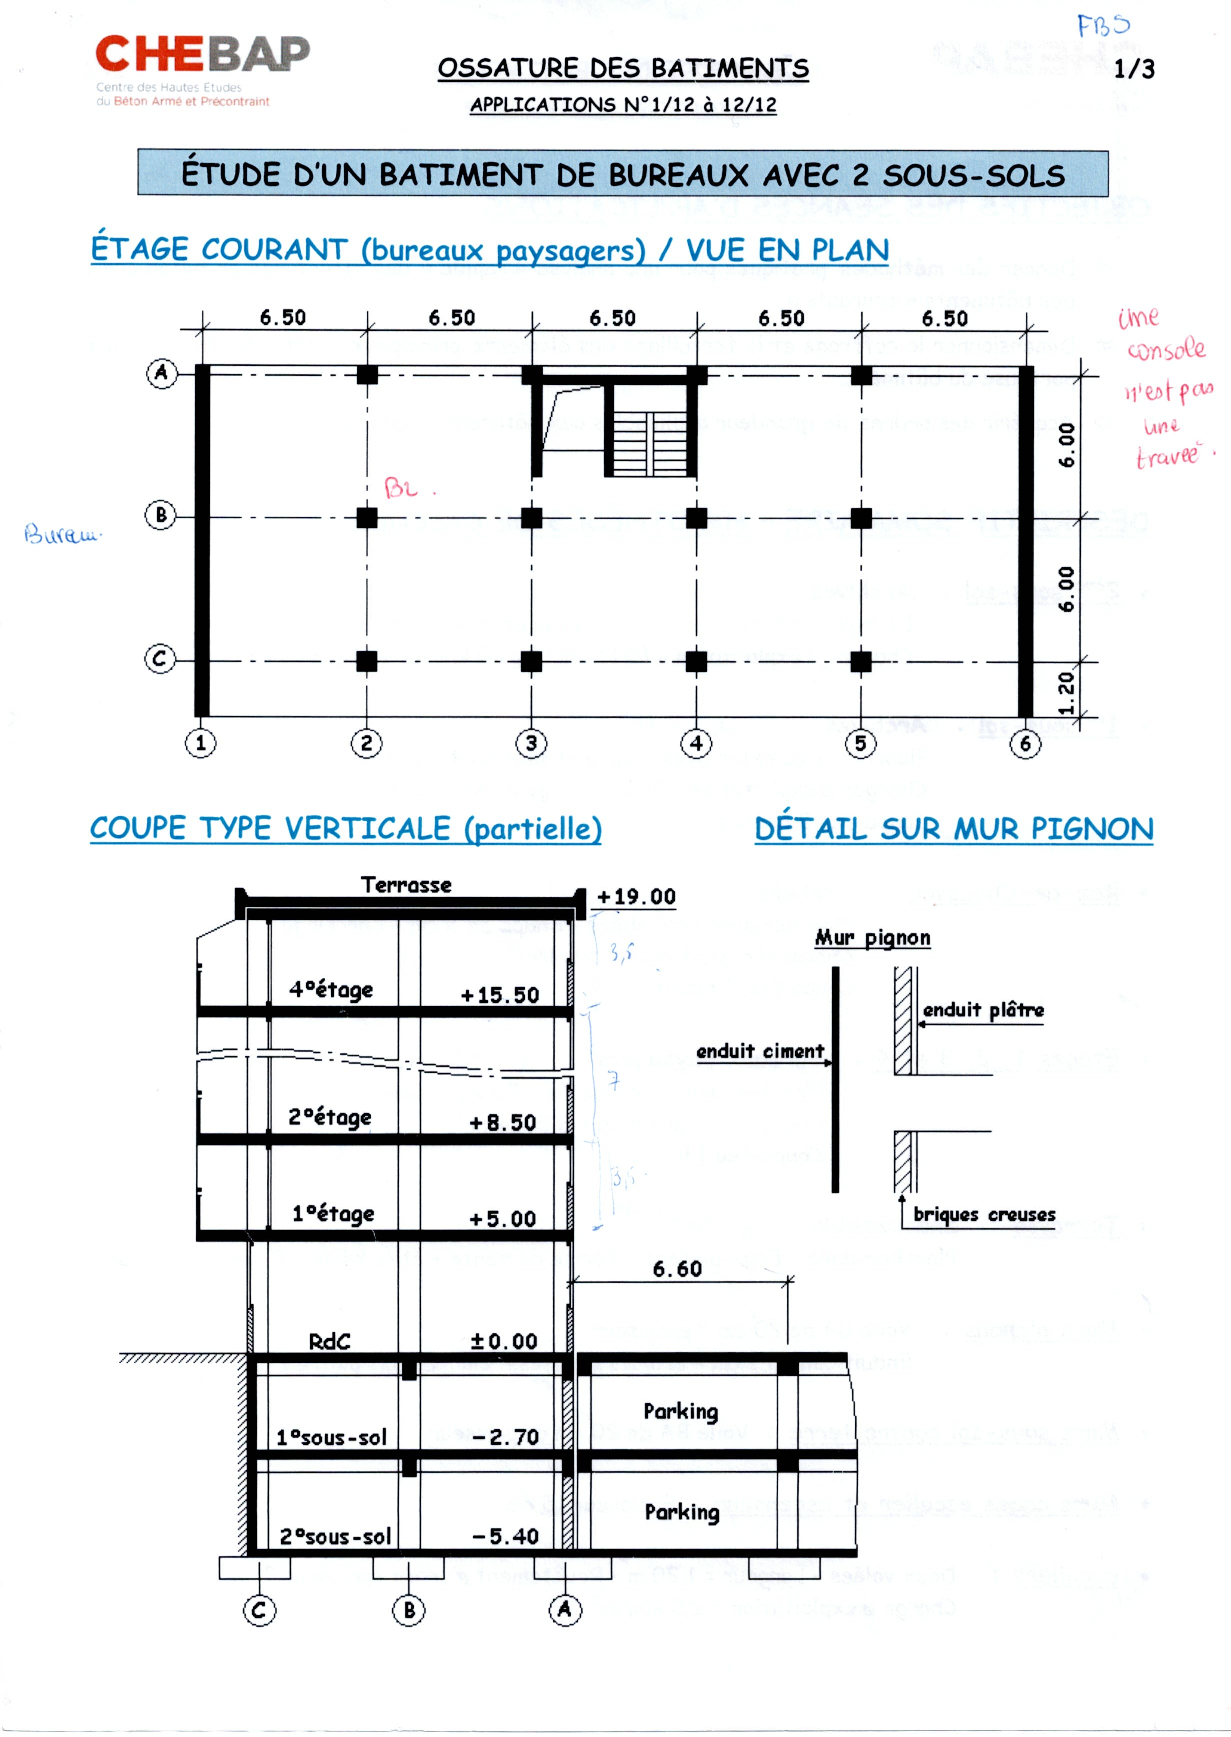
\includepdf[pages=-,pagecommand={\thispagestyle{plain}}]{meta/enonce.pdf}

\clearpage


% ════════════════ SÉANCES 1 À 12 ═════════════════════════════
% ════════════════════════════════════════════════════════════
% SÉANCE 1 — PRÉDIMENSIONNEMENT
% ════════════════════════════════════════════════════════════
\seance{1}{Prédimensionnement}

\subsection{Démarche générale}

Le prédimensionnement consiste à fixer une première estimation des dimensions des éléments porteurs de la structure, en partant des éléments \textbf{supportés} (qui ne reprennent que leur poids propre et les charges d'exploitation) pour aller progressivement vers les éléments qui en \textbf{supportent d'autres}. Dans le cadre de cette étude, le dimensionnement est mené dans l'ordre suivant :
\begin{itemize}
  \item dalles ;
  \item poutres secondaires ;
  \item poutres principales ;
  \item plancher-dalle (superstructure) et poteaux de superstructure (calcul itératif couplé) ;
  \item poteaux d'infrastructure.
\end{itemize}

\figureplaceholder{predim-vue-plan-batiment}{Vue en plan de la partie infrastructure du bâtiment : files A, B, C et 1 à 6 ; portées $L = 6{,}50$~m et $\ell = 6{,}00$~m}

Sur le plan architectural, on distingue \textbf{deux types de dalle} :
\begin{itemize}
  \item des \textbf{dalles nervurées} en infrastructure ;
  \item un \textbf{plancher-dalle} en superstructure.
\end{itemize}

\subsection{Dimensionnement des dalles nervurées (infrastructure)}

La surface de la dalle prédéfinie par le plan architectural est $6 \times 6{,}5$~m. Cependant, dans l'optique de soulager le travail de la dalle, des \textbf{poutres secondaires} sont ajoutées. Ainsi, la surface de calcul des dalles devient $6 \times 3{,}25$~m. La dalle qui fait l'objet du dimensionnement est celle du \textbf{1\textsuperscript{er} sous-sol} (cas le plus chargé : ses charges d'exploitation sont supérieures à celles des autres niveaux d'infrastructure). Les caractéristiques retenues seront ensuite appliquées à toutes les dalles d'infrastructure.

\subsubsection{Critère de flexibilité}

\[
\alpha = \frac{\ell_x}{\ell_y} = \frac{3{,}25}{6} = 0{,}542 \;>\; 0{,}4
\]

La dalle travaille donc \textbf{dans les deux sens}, et l'épaisseur minimale par flexibilité s'écrit :

\[
h_1 \;\geq\; \frac{\ell_x}{40} = \frac{3{,}25 \times 100}{40} \approx \mathbf{8{,}125~\text{cm}}
\]

\subsubsection{Critère de sécurité incendie}

La durée de coupe-feu requise pour le 1\textsuperscript{er} sous-sol étant de \textbf{2 heures}, l'épaisseur minimale est :

\[
h_2 \;\geq\; \mathbf{12~\text{cm}}
\]

\subsubsection{Critère de résistance}

Avec une classe de résistance C25/30 et un moment réduit $\mu = 0{,}2$, la condition de résistance s'écrit :

\[
d^2~(\text{cm}^2) \;\geq\; 3 \, M_u
\quad\text{avec}\quad
d = h - 3
\quad\text{et}\quad
M_u = \frac{P_u \, \ell_x^2}{10 \, (1 + 2\,\alpha^3)}
\]

Charge ELU de prédimensionnement :

\[
P_u = 1{,}35 \, P_p + 1{,}5 \, Q = 1{,}35 \times (0{,}12 \times 25) + 1{,}5 \times 10 \approx \mathbf{19{,}05~\text{kN/m}^2}
\]

D'où :

\[
M_u = \frac{19{,}05 \times 3{,}25^2}{10 \times (1 + 2 \times 0{,}542^3)} \approx \mathbf{15{,}3~\text{kN.m/m}}
\]

\[
d \;\geq\; \sqrt{3 \times 15{,}3} \approx 6{,}77~\text{cm}
\quad\Longrightarrow\quad
h_3 \;\geq\; 6{,}77 + 3 \approx \mathbf{9{,}77~\text{cm}}
\]

\subsubsection{Conclusion --- dalles nervurées}

\encadre{$h = \max\{h_1 \,;\, h_2 \,;\, h_3\} = \max\{8{,}125 \,;\, 12 \,;\, 9{,}77\} = \mathbf{12~\text{cm}}$}

\subsection{Dimensionnement des poutres secondaires}

Les poutres secondaires reportent les charges de la dalle vers les poutres principales. La poutre étudiée a une portée $L = 6$~m et reprend la dalle sur deux surfaces afférentes \textbf{trapézoïdales} de part et d'autre.

\figureplaceholder{predim-poutre-secondaire-charges}{Distribution des charges sur la poutre secondaire (surfaces afférentes trapézoïdales)}

\subsubsection{Critère de résistance en flexion}

La charge linéique équivalente sur la poutre secondaire vaut :

\[
P_u' = \left(0{,}5 - \frac{\alpha^2}{6}\right) \cdot 2 \, P_u \cdot \ell_x = \left(0{,}5 - \frac{0{,}542^2}{6}\right) \times 38{,}1 \times 3{,}25 \approx \mathbf{55{,}85~\text{kN/ml}}
\]

Le moment isostatique vaut :

\[
M_0 = \frac{P_u' \cdot L^2}{8} = \frac{55{,}85 \times 6^2}{8} \approx \mathbf{251{,}33~\text{kN.m}}
\]

D'où le moment ELU de prédimensionnement (forfaitaire) :

\[
M_u = 0{,}65 \, M_0 \approx \mathbf{163{,}4~\text{kN.m}}
\]

Pour $\mu = 0{,}2$ et C25/30, on a la condition $b_0 \, d^2 \geq 300 \, M_u$, avec l'hypothèse $b_0 \approx 0{,}4 \, d$ qui permet d'écrire :

\[
0{,}4 \, d^3 \;\geq\; 300 \, M_u
\quad\Longrightarrow\quad
d \;\geq\; \sqrt[3]{\frac{300 \, M_u}{0{,}4}} = \sqrt[3]{\frac{300 \times 163{,}4}{0{,}4}} \approx \mathbf{49{,}7~\text{cm}}
\]

D'où le choix : $d = 50$~cm, $b_0 = 0{,}4 \times 50 = 20$~cm, et $h = d + 5 = 55$~cm.

\subsubsection{Critère de résistance à l'effort tranchant}

L'effort tranchant maximal en appui s'écrit :

\[
V_0 = R_A = R_B = \frac{1}{2} \cdot \frac{6 + 2{,}75}{2} \cdot 38{,}1 \approx \mathbf{83{,}3~\text{kN}}
\]

Vérification de la condition $V_0 \leq 0{,}3 \, b_0 \, d$ :

\[
83{,}3 \;\leq\; 0{,}3 \times 20 \times 50 = 300 \quad \checkmark
\]

Vérification de la contrainte de cisaillement :

\[
\tau = \frac{3}{2} \cdot \frac{V_0}{b \, h} = \frac{3}{2} \times \frac{83{,}3}{20 \times 55} \approx 1{,}13~\text{MPa} \;\leq\; 3~\text{MPa} \quad \checkmark
\]

\subsubsection{Critère de flexibilité}

\[
h \;\geq\; \frac{L}{16} \quad\Longrightarrow\quad 55 \;\geq\; \frac{600}{16} = 37{,}5~\text{cm} \quad \checkmark
\]

\subsubsection{Conclusion --- poutres secondaires}

\encadre{Section retenue : $\mathbf{b_0 = 20~\text{cm}}$ ; $\mathbf{d = 50~\text{cm}}$ ; $\mathbf{h = 55~\text{cm}}$}

\subsection{Dimensionnement des poutres principales}

À partir du schéma de distribution des charges, la poutre principale supporte :
\begin{itemize}
  \item le poids propre de la dalle qui la surplombe (\textcircled{1} sur le schéma) ;
  \item les charges apportées par les surfaces afférentes triangulaires (\textcircled{2}) ;
  \item les poutres secondaires qui s'y appuient (\textcircled{3}) ;
  \item les charges de dalle apportées par les surfaces afférentes trapézoïdales (\textcircled{4}).
\end{itemize}

Pour simplifier le prédimensionnement, on retient un schéma simplifié de descente de charges (schéma rectangulaire \textcircled{2}), reportant une charge concentrée au milieu de la travée principale.

\figureplaceholder{predim-poutre-principale-charges}{Schémas de distribution des charges sur la poutre principale : modèle complet (gauche) et simplifié (droite)}

\subsubsection{Bilan des charges}

\begin{itemize}
  \item \textbf{Poutre secondaire (poutrelle)} : $P_p = 0{,}2 \times 0{,}55 \times 6 \times 25 \approx \mathbf{16{,}5~\text{kN}}$
  \item \textbf{Dalle} : $P_D = 19{,}05 \times 6 \times 3{,}25 \approx \mathbf{371{,}48~\text{kN}}$
  \item \textbf{Charge totale supportée} :
\end{itemize}

\[
P_t = P_D + 1{,}35 \, P_p = 371{,}48 + 1{,}35 \times 16{,}5 \approx \mathbf{393{,}76~\text{kN}}
\]

\subsubsection{Critère de résistance en flexion}

Le schéma statique est celui d'une poutre simplement appuyée de portée $L = 6{,}5$~m, soumise à la charge concentrée $P_t$ à mi-travée. Le moment isostatique en travée vaut :

\[
M_0 = \frac{P_t \cdot L}{4} = \frac{393{,}76 \times 6{,}5}{4} \approx \mathbf{639{,}86~\text{kN.m}}
\]

\[
M_u = 0{,}65 \, M_0 \approx \mathbf{415{,}91~\text{kN.m}}
\]

De la même manière que pour les poutres secondaires (avec $\mu = 0{,}2$ et $b_0 \approx 0{,}4 \, d$) :

\[
d \;\geq\; \sqrt[3]{\frac{300 \, M_u}{0{,}4}} = \sqrt[3]{\frac{300 \times 415{,}91}{0{,}4}} \approx \mathbf{67{,}82~\text{cm}}
\]

D'où $d \approx 68$~cm, $b_0 \approx 0{,}4 \times 68 = 27{,}2 \approx 30$~cm, et $h = d + 5 \approx 73$~cm.

\paragraph{Limitation de gabarit}

En raison de la limitation du \textbf{gabarit sous poutres à 2~m} pour les sous-sols, la hauteur de la poutre est ramenée à $h = 70$~cm. Au-delà de cette valeur, on dépasserait le gabarit autorisé. Avec $h = 70$~cm, on a $d = h - 5 = 65$~cm.

\subsubsection{Critère de résistance à l'effort tranchant}

\[
V_0 = \frac{P_t}{2} = \frac{393{,}76}{2} \approx 196{,}88~\text{kN}
\]

\[
V_0 \;\leq\; 0{,}3 \, b_0 \, d \quad\Longrightarrow\quad 196{,}88 \;\leq\; 0{,}3 \times 30 \times 65 = 585~\text{kN} \quad \checkmark
\]

\subsubsection{Critère de sécurité incendie}

Coupe-feu de 2 heures :

\[
b_0 \;\geq\; 30~\text{cm} \;\geq\; 20~\text{cm} \quad \checkmark
\]

\subsubsection{Critère de flexibilité}

\[
h = 70~\text{cm} \;\geq\; \frac{L}{16} = \frac{650}{16} \approx 40{,}63~\text{cm} \quad \checkmark
\]

\subsubsection{Conclusion --- poutres principales}

\encadre{Section retenue : $\mathbf{b_0 = 30~\text{cm}}$ ; $\mathbf{d = 65~\text{cm}}$ ; $\mathbf{h = 70~\text{cm}}$}

\subsection{Dimensionnement du plancher-dalle et des poteaux de superstructure}

Les dimensionnements du plancher-dalle (superstructure) et des poteaux qui le supportent sont \textbf{couplés} : l'épaisseur de la dalle dépend de la géométrie des poteaux, et inversement. Ce couplage est résolu par un calcul \textbf{itératif} jusqu'à convergence des valeurs.

Dans le cadre de cette étude, deux itérations sont effectuées :
\begin{itemize}
  \item une première tentative qui ne converge pas ;
  \item une seconde tentative qui montre la convergence.
\end{itemize}

Pour le dimensionnement du poteau de superstructure, on considère le poteau de la \textbf{file B au RDC}, dont la surface afférente vaut $S = 6 \times 6{,}5 = 39$~m\textsuperscript{2}. En tenant compte de la \textbf{continuité} des travées (majoration de 15\%) :

\[
S^* = 1{,}15 \times S = \mathbf{44{,}85~\text{m}^2}
\]

\subsubsection{Première tentative --- \texorpdfstring{$h = 25$}{h = 25}~cm}

\paragraph{Critère de flexibilité du plancher-dalle}~

\[
h \;\geq\; \frac{L}{30} = \frac{650}{30} \approx 21{,}66~\text{cm} \quad\Longrightarrow\quad h \approx \mathbf{25~\text{cm}}
\]

\paragraph{Descente de charges (avec $h = 0{,}25$~m)}~

\textbf{Terrasse :} $G_1 = (0{,}25 \times 25) + 0{,}4 + 2 + 0{,}1 + (0{,}06 \times 15) \approx \mathbf{9{,}65~\text{kN/m}^2}$

\textbf{Étage courant :} $G_2 = 4 \times \big[(0{,}25 \times 25) + 0{,}4 + 0{,}1\big] = \mathbf{27~\text{kN/m}^2}$ (sur 4 étages)

\textbf{Charges d'exploitation :} $Q = 3{,}5$~kN/m\textsuperscript{2}

\paragraph{Critère effort tranchant}~

\[
P_u = 1{,}35 \times \big[(0{,}25 \times 25) + 0{,}4 + 0{,}1\big] + 1{,}5 \times 3{,}5 \approx \mathbf{14{,}36~\text{kN/m}^2}
\]

\[
V_u = P_u \cdot \frac{\ell \cdot L}{4} = 14{,}36 \times \frac{6 \times 6{,}5}{4} \approx \mathbf{140{,}01~\text{kN}}
\]

La condition $(b + h) \, h \geq 15 \, V_u$ donne :

\[
b \;\geq\; \frac{15 \, V_u}{h} - h = \frac{15 \times 140{,}01}{25} - 25 \approx \mathbf{59~\text{cm}}
\]

\paragraph{Vérification de l'effort normal}~

\[
N_u = \big[1{,}35 \, G + 1{,}5 \, Q\big] \cdot S^* = \big[1{,}35 \times (9{,}65 + 27) + 1{,}5 \times 3{,}5\big] \times 44{,}85 \approx \mathbf{2\,454{,}53~\text{kN}}
\]

\[
1{,}3 \, B \;\geq\; N_u \quad\Longrightarrow\quad B \;\geq\; \frac{N_u}{1{,}3} \quad\Longrightarrow\quad b \;\geq\; \sqrt{\frac{N_u}{1{,}3}} \approx \mathbf{43{,}45~\text{cm}}
\]

\paragraph{Conclusion de la 1\textsuperscript{re} tentative}~

\textbf{Pas de convergence} : les dimensions adoptées pour le plancher-dalle conduisent à des poteaux trop élancés pour reprendre l'effort tranchant. Il faut donc \textbf{augmenter l'épaisseur de la dalle}.

\subsubsection{Seconde tentative --- \texorpdfstring{$h = 29$}{h = 29}~cm}

On augmente l'épaisseur du plancher-dalle à $h = 29$~cm.

\paragraph{Descente de charges (avec $h = 0{,}29$~m)}~

\textbf{Terrasse :} $G_1 = (0{,}29 \times 25) + 0{,}4 + 2 + 0{,}1 + (0{,}06 \times 15) \approx \mathbf{10{,}65~\text{kN/m}^2}$

\textbf{Étage courant :} $G_2 = 4 \times \big[(0{,}29 \times 25) + 0{,}4 + 0{,}1\big] = \mathbf{31~\text{kN/m}^2}$

\textbf{Charges d'exploitation :} $Q = 3{,}5$~kN/m\textsuperscript{2}

\paragraph{Critère effort tranchant}~

\[
V_u = \big[1{,}35 \times (0{,}29 \times 25 + 0{,}4 + 0{,}1) + 1{,}5 \times 3{,}5\big] \times \frac{6 \times 6{,}5}{4} \approx \mathbf{153{,}2~\text{kN}}
\]

\[
b \;\geq\; \frac{15 \times 153{,}2}{29} - 29 \approx \mathbf{50~\text{cm}}
\]

\paragraph{Vérification de l'effort normal}~

\[
N_u = 44{,}85 \times \big[1{,}35 \times (10{,}65 + 31) + 1{,}5 \times 3{,}5\big] \approx \mathbf{2\,757{,}3~\text{kN}}
\]

\[
b \;\geq\; \sqrt{\frac{N_u}{1{,}3}} = \sqrt{\frac{2\,757{,}3}{1{,}3}} \approx \mathbf{46~\text{cm}}
\]

\paragraph{Conclusion de la 2\textsuperscript{e} tentative}~

\textbf{Convergence atteinte} : les deux critères donnent $b \approx 50$~cm, valeur compatible avec $h = 29$~cm pour la dalle.

\encadre{Plancher-dalle : $\mathbf{h = 29~\text{cm}}$}
\encadre{Poteau de superstructure : $\mathbf{b \times h = 50 \times 50~\text{cm}^2}$}

\subsection{Dimensionnement des poteaux d'infrastructure}

On considère le poteau de la file \textbf{B au 2\textsuperscript{e} sous-sol} (le plus chargé, car il reprend la totalité des étages supérieurs et les charges des deux niveaux de sous-sol). Sa surface afférente est identique : $S^* = 44{,}85$~m\textsuperscript{2}.

\subsubsection{Descente de charges supplémentaire}

L'effort normal apporté par les étages courants (déjà calculé en superstructure) vaut $N_{u,1} = 2\,757{,}3$~kN. À cet effort s'ajoutent les contributions du 1\textsuperscript{er} et du 2\textsuperscript{e} sous-sol.

\paragraph{Niveau du 1\textsuperscript{er} sous-sol (plancher avec retombées)}~

Charges permanentes :
\begin{align*}
G &= P_{dalle} + P_{chape} + P_{carrelage} + P_{poutre\,principale} + P_{poutre\,secondaire} \\
&= 44{,}85 \times \big[(0{,}12 \times 25) + (20 \times 0{,}03) + 0{,}5\big] + (25 \times 0{,}58 \times 0{,}3 \times 6{,}5) + (0{,}43 \times 25 \times 0{,}2 \times 6) \\
&\approx \mathbf{225{,}1~\text{kN}}
\end{align*}

Charges d'exploitation : $Q = 5 \times 44{,}85 \approx 224{,}3$~kN.

\[
N_{u,2} = 1{,}35 \, G + 1{,}5 \, Q = 1{,}35 \times 225{,}1 + 1{,}5 \times 224{,}3 \approx \mathbf{640{,}34~\text{kN}}
\]

\paragraph{Niveau du 2\textsuperscript{e} sous-sol (dallage)}~

\[
G = 44{,}85 \times (0{,}12 \times 25) + (25 \times 0{,}58 \times 0{,}3 \times 6{,}5) + (0{,}43 \times 25 \times 0{,}2 \times 6) \approx \mathbf{175{,}73~\text{kN}}
\]

Charges d'exploitation (archives, $Q = 10$~kN/m\textsuperscript{2}) : $Q = 10 \times 44{,}85 = 448{,}5$~kN.

\[
N_{u,3} = 1{,}35 \times 175{,}73 + 1{,}5 \times 448{,}5 \approx \mathbf{909{,}99~\text{kN}}
\]

\subsubsection{Effort normal total et critère de résistance}

\[
N_u = N_{u,1} + N_{u,2} + N_{u,3} = 2\,757{,}3 + 640{,}34 + 909{,}99 \approx \mathbf{4\,307{,}63~\text{kN}}
\]

Pour un poteau carré $B = b^2$ et la condition $1{,}3 \, B \geq N_u$ :

\[
b \;\geq\; \sqrt{\frac{N_u}{1{,}3}} = \sqrt{\frac{4\,307{,}63}{1{,}3}} \approx \mathbf{57{,}6~\text{cm}}
\]

\subsubsection{Critère de sécurité incendie}

Au niveau du 2\textsuperscript{e} sous-sol, la durée de coupe-feu requise est de \textbf{2 heures}. Le tableau des dimensions minimales de poteau donne $b \geq 35$~cm, ce qui est moins contraignant que le critère de résistance précédent.

\subsubsection{Conclusion --- poteau d'infrastructure}

\encadre{Poteau d'infrastructure : $\mathbf{b \times h = 60 \times 60~\text{cm}^2}$}

\subsection{Synthèse du prédimensionnement}

\begin{center}
\begin{tabularx}{0.85\linewidth}{Xc}
\toprule
\textbf{Élément} & \textbf{Dimensions retenues} \\
\midrule
Dalle nervurée (infrastructure)             & $h = 12$~cm \\
Plancher-dalle (superstructure)             & $h = 29$~cm \\
Poutre secondaire (infrastructure)          & $20 \times 55$~cm\textsuperscript{2} \\
Poutre principale (infrastructure)          & $30 \times 70$~cm\textsuperscript{2} \\
Poteau de superstructure                    & $50 \times 50$~cm\textsuperscript{2} \\
Poteau d'infrastructure                     & $60 \times 60$~cm\textsuperscript{2} \\
\bottomrule
\end{tabularx}
\end{center}

Ces dimensions servent de \textbf{base} à toutes les analyses ultérieures (descente de charges, dimensionnement des éléments, vérifications au feu, etc.). En particulier, l'épaisseur du plancher-dalle ($h = 29$~cm) intervient directement dans le calcul des charges permanentes (Séance 2), et les dimensions des poteaux conditionnent les surfaces tributaires et les vérifications au poinçonnement (Séances 11 \& 12).


% ════════════════════════════════════════════════════════════
% SÉANCE 2 — DESCENTE DE CHARGES
% ════════════════════════════════════════════════════════════
\seance{2}{Descente de charges}

\subsection{Définition et principe}

La descente de charges consiste à \textbf{cumuler, niveau par niveau, l'ensemble des charges} (permanentes et d'exploitation) qui sollicitent un élément porteur, depuis la toiture jusqu'aux fondations. Elle permet de déterminer l'effort normal et le moment au pied de chaque poteau ou voile, et constitue la base de tout dimensionnement structural.

Avant de commencer les calculs, il faut identifier le \textbf{poteau le plus sollicité}. Ce choix n'est pas arbitraire : c'est toujours le poteau qui supporte la plus grande surface de plancher autour de lui, appelée \textbf{surface tributaire} (ou surface afférente).

Dans cette étude, la descente de charges est effectuée sur le \textbf{poteau de la file B2 au 2\textsuperscript{e} sous-sol}, le plus chargé du bâtiment.

\subsection{Réduction des charges d'exploitation}

L'Eurocode autorise deux types de réductions sur les charges d'exploitation : selon l'aire portée et selon le nombre d'étages.

\subsubsection{Réduction selon l'aire portée \texorpdfstring{($\alpha_A$)}{(αA)}}

\[
  \alpha_A = 0{,}77 + \frac{3{,}5}{A} \leq 1{,}0
\]

Pour la descente de charges, on prend par sécurité :
\[
  \boxed{\alpha_A = 1{,}0}
\]

\subsubsection{Réduction selon le nombre d'étages \texorpdfstring{($\alpha_n$)}{(αn)}}

Plus il y a d'étages au-dessus d'un niveau, plus la probabilité d'occupation maximale simultanée à \emph{tous} les étages diminue. On applique donc une réduction (formule FDP 18-717, catégorie B = bureaux) :
\[
  \alpha_n = 0{,}7 + \frac{0{,}8}{n} \leq 1{,}0
\]

où $n$ = nombre d'étages de \emph{même catégorie} situés \emph{au-dessus} du niveau étudié.

\begin{figure}[H]\centering
  
\includegraphics[width=0.75\linewidth]{s2-fig01-vue-elevation-batiment.png}
  \caption{Vue en élévation du bâtiment : niveaux et coefficients de réduction $\alpha_n$}
  \label{fig:s2-vue-elevation}
\end{figure}

\paragraph{Application :}
\begin{itemize}
  \item 4\textsuperscript{e} étage ($n = 1$) : $\alpha_n = 0{,}7 + 0{,}8/1 = 1{,}5 \to$ limité à $1{,}0$ (pas de réduction)
  \item 3\textsuperscript{e} étage ($n = 2$) : $\alpha_n = 0{,}7 + 0{,}8/2 = 1{,}1 \to$ limité à $1{,}0$ (pas de réduction)
  \item 2\textsuperscript{e} étage ($n = 3$) : $\alpha_n = 0{,}7 + 0{,}8/3 = 0{,}967$ (réduction appliquée)
  \item 1\textsuperscript{er} étage ($n = 4$) : $\alpha_n = 0{,}7 + 0{,}8/4 = 0{,}90$ (réduction appliquée)
  \item RDC et sous-sol : catégories \emph{différentes} (ateliers et archives) $\to$ pas de réduction $\alpha_n$.
\end{itemize}

\subsection{Surface tributaire du poteau B2}

Le poteau B2 est un poteau intérieur. Sa surface tributaire correspond aux demi-portées des travées qui le bordent.

D'après le plan : travées de 6,50\,m en direction $X$ et 6,00\,m en direction $Y$.
\[
  S = 6{,}50 \times 6{,}00 = \mathbf{39{,}00~\text{m}^2}
\]

\subsection{Charges permanentes par m\texorpdfstring{$^2$}{2}}

\begin{figure}[H]\centering
  
\includegraphics[width=0.75\linewidth]{s2-fig02-charges-permanentes-coupe.png}
  \caption{Schéma des charges permanentes : descente depuis la dalle vers la poutrelle, la retombée et le poteau}
  \label{fig:s2-charges-permanentes}
\end{figure}

\paragraph{Terrasse inaccessible :}
\[
\begin{aligned}
  g &= 7{,}25 + 0{,}40 + 2{,}00 + 0{,}10 + 0{,}90 \\
    &= \mathbf{10{,}65~\text{kN/m}^2}
\end{aligned}
\]

\paragraph{Étage courant (bureaux) :}
\[
  g = 7{,}25 + 0{,}10 + 0{,}40 = \mathbf{7{,}75~\text{kN/m}^2}
\]

\paragraph{RDC (plancher haut du 1\textsuperscript{er} sous-sol, dalle nervurée 12\,cm) :}
\[
  g = 0{,}12 \times 25 + 0{,}03 \times 20 + 0{,}50 = 3{,}00 + 0{,}60 + 0{,}50 = \mathbf{4{,}10~\text{kN/m}^2}
\]

\paragraph{1\textsuperscript{er} sous-sol (dalle 12\,cm sans chape ni revêtement) :}
\[
  g = 0{,}12 \times 25 = \mathbf{3{,}00~\text{kN/m}^2}
\]

\subsection{Poids propres linéiques}

\begin{center}
\begin{tabular}{lr}
\toprule
Élément & Charge (kN/ml) \\
\midrule
Poutrelle 20$\times$43\,cm : $0{,}43 \times 0{,}20 \times 25$ & 2,15 \\
Poutre principale 30$\times$58\,cm : $0{,}30 \times 0{,}58 \times 25$ & 4,35 \\
Poteau superstructure 50$\times$50\,cm : $0{,}50 \times 0{,}50 \times 25$ & 6,25 \\
Poteau infrastructure 60$\times$60\,cm : $0{,}60 \times 0{,}60 \times 25$ & 9,00 \\
\bottomrule
\end{tabular}
\end{center}

\textbf{Remarque.} Les retombées 0,43\,m et 0,58\,m correspondent à la partie de la poutre située \emph{sous} la dalle :
\begin{itemize}
  \item Poutre principale : $h_\text{totale} = 70$\,cm $-$ dalle 12\,cm $= 58$\,cm
  \item Poutre secondaire : $h_\text{totale} = 55$\,cm $-$ dalle 12\,cm $= 43$\,cm
\end{itemize}

\subsection{Cumul des charges permanentes \texorpdfstring{$G$}{G} sur le poteau B2}

Pour chaque niveau, on additionne :
\begin{itemize}
  \item la charge surfacique du plancher $\times$ surface tributaire (39\,m\textsuperscript{2}),
  \item les retombées de poutres $\times$ longueurs respectives,
  \item le poids propre du poteau du niveau.
\end{itemize}

\subsubsection{Terrasse}
\[
\begin{aligned}
  G_\text{terrasse} &= 10{,}65 \times 39 + 2{,}15 \times 6{,}50 + 4{,}35 \times 6{,}00 + 6{,}25 \times 3{,}50 \\
                    &= 415{,}4 + 14{,}0 + 26{,}1 + 21{,}9 \\
                    &= 477{,}4 \approx \mathbf{500~\text{kN}}
\end{aligned}
\]

\subsubsection{Étage courant (4\texorpdfstring{\textsuperscript{e}}{e}, 3\texorpdfstring{\textsuperscript{e}}{e}, 2\texorpdfstring{\textsuperscript{e}}{e} étages)}
\[
\begin{aligned}
  G_\text{étage} &= 7{,}75 \times 39 + 14{,}0 + 26{,}1 + 21{,}9 \\
                 &= 302{,}3 + 62{,}0 \\
                 &= 364{,}3 \approx \mathbf{368~\text{kN}}
\end{aligned}
\]

\subsubsection{1\texorpdfstring{\textsuperscript{er}}{er} étage}

Le poteau du 1\textsuperscript{er} étage a une hauteur supérieure de 10\,cm pour rejoindre le RDC :
\[
\begin{aligned}
  G_{1^\text{er}\text{ étage}} &= 7{,}75 \times 39 + 14{,}0 + 26{,}1 + 6{,}25 \times 3{,}60 \\
                                &= 302{,}3 + 14{,}0 + 26{,}1 + 22{,}5 \\
                                &= 364{,}9 \approx \mathbf{377~\text{kN}}
\end{aligned}
\]

\subsubsection{Rez-de-chaussée}

Le poteau passe en infrastructure (60$\times$60). On ajoute une estimation de 40\,kN pour les murs et allèges.
\[
\begin{aligned}
  G_\text{RDC} &= 4{,}10 \times 39 + 14{,}0 + 26{,}1 + 9{,}00 \times 2{,}70 + 40{,}0 \\
               &= 159{,}9 + 14{,}0 + 26{,}1 + 24{,}3 + 40{,}0 \\
               &= 264{,}3 \approx \mathbf{264~\text{kN}}
\end{aligned}
\]

\subsubsection{1\texorpdfstring{\textsuperscript{er}}{er} sous-sol}

On ajoute 33,6\,kN pour les murs voiles BA du sous-sol :
\[
\begin{aligned}
  G_\text{SS1} &= 3{,}00 \times 39 + 14{,}0 + 26{,}1 + 24{,}3 + 33{,}6 \\
               &= 117{,}0 + 14{,}0 + 26{,}1 + 24{,}3 + 33{,}6 \\
               &= \mathbf{215{,}0~\text{kN}}
\end{aligned}
\]

\subsection{Charges d'exploitation \texorpdfstring{$Q$}{Q}}

Les charges $Q$ sont calculées en multipliant la charge surfacique par la surface tributaire $S = 39$\,m\textsuperscript{2}, puis \textbf{majorées par le coefficient de continuité} $\times 1{,}15$ pour tenir compte des reports de charges des travées adjacentes (FDP 18-717).

\begin{center}
\begin{tabular}{lrrr}
\toprule
Niveau & $q$ (kN/m\textsuperscript{2}) & $q \times S$ (kN) & $\times 1{,}15$ (kN) \\
\midrule
Terrasse (inaccessible)            & 0    & 0     & \textbf{0}   \\
Étages bureaux                     & 3,5  & 136,5 & \textbf{157} \\
RDC ateliers                       & 5,0  & 195,0 & \textbf{224} \\
1\textsuperscript{er} SS archives  & 10,0 & 390,0 & \textbf{449} \\
\bottomrule
\end{tabular}
\end{center}

\subsection{Tableau récapitulatif de la descente de charges}

On cumule $G$ et $Q$ niveau par niveau, du haut vers le bas. La colonne $\Sigma Q_\text{réduit}$ applique le coefficient $\alpha_n$.

\vspace{4pt}
\begin{center}
\renewcommand{\arraystretch}{1.4}
\begin{tabular}{lrrrrrr}
\toprule
\textbf{Niveau} & \textbf{$G$} & \textbf{$Q$} & \textbf{$\Sigma G$} & \textbf{$\Sigma Q$ brut} & \textbf{$\alpha_n$} & \textbf{$\Sigma Q$ réduit} \\
                & (kN)         & (kN)         & (kN)                & (kN)                     &                     & (kN) \\
\midrule
Terrasse                            & 500 & 0   & 500    & 0      & ---   & 0      \\
4\textsuperscript{e} étage          & 368 & 157 & 868    & 157    & 1,0   & 157    \\
3\textsuperscript{e} étage          & 368 & 157 & 1\,236 & 314    & 1,0   & 314    \\
2\textsuperscript{e} étage          & 368 & 157 & 1\,604 & 471    & 0,967 & 455    \\
1\textsuperscript{er} étage         & 377 & 157 & 1\,981 & 628    & 0,90  & 565    \\
RDC                                 & 264 & 224 & 2\,245 & 852    & ---   & 789    \\
1\textsuperscript{er} sous-sol      & 215 & 449 & 2\,460 & 1\,301 & ---   & 1\,238 \\
\bottomrule
\end{tabular}
\end{center}
\vspace{4pt}

\subsection{Conclusion}

Au pied du poteau B2 (au niveau du 2\textsuperscript{e} sous-sol), les charges de calcul sont :

\encadre{$\Sigma G = 2\,460~\text{kN}$ \qquad $\Sigma Q_\text{réduit} = 1\,238~\text{kN}$}

Ces valeurs serviront de base au dimensionnement des fondations en Séance 3.


% ════════════════════════════════════════════════════════════
% SÉANCE 3 — SEMELLES DE FONDATIONS
% ════════════════════════════════════════════════════════════
\seance{3}{Semelles de fondations}

\subsection{Définition et choix du type de fondation}

Les fondations sont les éléments de la structure qui assurent la transmission au sol des charges issues de la superstructure et de l'infrastructure. Leur dimensionnement est une étape critique du projet : elles doivent à la fois reprendre l'effort normal cumulé issu de la descente de charges, limiter les tassements à des valeurs compatibles avec le bon fonctionnement de l'ouvrage, et résister aux sollicitations particulières (excentrement, poinçonnement, glissement).

On distingue classiquement deux grandes familles :
\begin{itemize}
  \item les \textbf{fondations superficielles} (semelles isolées, filantes ou radiers), utilisées lorsque le sol porteur est rencontré à faible profondeur et que sa contrainte admissible est suffisante~;
  \item les \textbf{fondations profondes} (pieux, barrettes, micropieux), utilisées lorsque le bon sol est situé en profondeur, ou lorsque les charges sont trop importantes pour une fondation superficielle.
\end{itemize}

Pour le présent projet, le rapport géotechnique fournit deux contraintes admissibles, correspondant aux deux solutions envisageables :
\begin{itemize}
  \item solution sur \textbf{semelles superficielles} : $q_a = 0{,}75$\,MPa à l'ELU~;
  \item solution sur \textbf{pieux} : $\sigma_{ELS} = 5{,}0$\,MPa à l'ELS.
\end{itemize}

Le bâtiment sera \textbf{fondé sur deux pieux} sous chaque poteau de la file B. Ce choix est motivé par les charges importantes transmises par le poteau B2 (le plus chargé du bâtiment) et par la volonté de limiter les tassements différentiels. Le dimensionnement de cette solution est détaillé en premier ci-après. À titre de comparaison, la solution alternative sur semelle superficielle isolée est ensuite présentée.

\paragraph{Rappel des charges au pied du poteau B2.} Issues de la Séance~2 :

\encadre{$\Sigma G = 2\,460~\text{kN}$ \qquad $\Sigma Q_\text{réduit} = 1\,238~\text{kN}$}

% ─────────────────────────────────────────────────────────────
\subsection{Solution retenue --- Fondation sur deux pieux}
% ─────────────────────────────────────────────────────────────

\begin{figure}[H]\centering
  
\includegraphics[width=0.95\linewidth]{s3-fig01-semelle-2-pieux-vue-coupe.png}
  \caption{Principe d'une semelle sur deux pieux : vue en plan (gauche) et coupe en élévation (droite). $N_{Ed}$ : effort normal du poteau ; $R$ : réaction de chaque pieu ; $b_0$ : largeur de la semelle ; $\ell_t$ : entraxe des pieux}
  \label{fig:s3-semelle-principe}
\end{figure}

\subsubsection{Justification du choix de deux pieux}

Le poteau B2 pourrait théoriquement être fondé sur un seul pieu. Cependant, le risque d'\textbf{excentrement} entre l'effort normal du poteau et l'axe du pieu est très probable lors de l'exécution. Cet excentrement engendrerait une sollicitation parasite en flexion du pieu, qui n'est ni adaptée à ce type d'élément, ni économique à reprendre par armatures. Pour cette raison, le bâtiment sera fondé sur \textbf{deux pieux} reliés par une semelle de liaison rigide.

\subsubsection{Effort normal repris par chaque pieu et diamètre des pieux}

L'effort normal majoré transmis par le poteau, à reprendre par l'ensemble \emph{semelle + pieux}, s'écrit, en majorant de 5\,\% pour tenir compte du poids propre de la semelle de liaison et des incertitudes :
\[
  N_{Ed} = 1{,}05\,(\Sigma G + \Sigma Q_\text{réd}) = 1{,}05 \times (2\,460 + 1\,238) = \mathbf{3\,883~\text{kN}}
\]

Comme le montre le schéma précédent, l'effort normal repris par chaque pieu correspond à la réaction $R$ telle que :
\[
  R = \frac{N_{Ed}}{2} = \frac{3\,883}{2} = \mathbf{1\,941{,}5~\text{kN}}
\]

\paragraph{Diamètre des pieux.} La condition à respecter est :
\[
  \sigma_\text{pieux} = \frac{R}{S_\text{pieux}} \leq \sigma_{ELS}
  \quad\Longrightarrow\quad
  S_\text{pieux} \geq \frac{R}{\sigma_{ELS}} = \frac{1{,}9415}{5} = 0{,}3883~\text{m}^2
\]

Le pieu étant de section circulaire :
\[
  S_\text{pieux} = \frac{\pi\,D_\text{pieux}^{2}}{4}
  \quad\Longrightarrow\quad
  D_\text{pieux} = \sqrt{\frac{4 \times 0{,}3883}{\pi}} = 0{,}703~\text{m}
\]

\encadre{$D_\text{pieux} = 0{,}70$~m}

\subsubsection{Géométrie de la semelle de liaison}

\paragraph{Entraxe et longueur.} L'entraxe des pieux est usuellement pris égal à $2{,}5\,D_\text{pieux}$ pour assurer une bonne diffusion des charges et limiter l'effet de groupe :
\[
  l_t = 2{,}5 \times 0{,}70 = \mathbf{1{,}75~\text{m}}
\]

La longueur $L$ de la semelle est déduite en débordant de chaque côté d'une demi-section de pieu plus 5\,cm de débord :
\[
  L = l_t + D_\text{pieux} + 10~\text{cm} = 1{,}75 + 0{,}70 + 0{,}10 = \mathbf{2{,}55~\text{m}}
\]

\paragraph{Largeur.} La largeur $b_0$ de la semelle est prise comme la plus grande dimension entre le poteau et le pieu, augmentée d'un débord de 10\,cm :
\[
  b_0 = \max\{b_\text{poteau} ;\, D_\text{pieux}\} + 10~\text{cm} = \max\{0{,}60 ;\, 0{,}70\} + 0{,}10 = \mathbf{0{,}80~\text{m}}
\]

\paragraph{Hauteur utile et hauteur totale.} La hauteur utile est calculée par la méthode des bielles avec un angle d'inclinaison de bielle $\theta = 55^\circ$ :
\[
  d = \left(\frac{l_t}{2} - \frac{a}{4}\right)\,\tan\theta
    = \left(\frac{1{,}75}{2} - \frac{0{,}60}{4}\right) \tan 55^\circ
    = 0{,}725 \times 1{,}4281 = \mathbf{1{,}035~\text{m}}
\]

avec $a$ = côté du poteau (60\,cm). La hauteur totale est obtenue en ajoutant l'enrobage et le rayon des armatures :
\[
  h = d + 5~\text{cm} = \mathbf{1{,}10~\text{m}}
\]

\begin{figure}[H]\centering
  
\includegraphics[width=0.65\linewidth]{s3-fig02-methode-bielles.png}
  \caption{Méthode des bielles --- demi-coupe transversale : l'effort $N_{Ed}$ se transmet par une bielle inclinée jusqu'à l'axe du pieu, équilibrée par un tirant horizontal $F$ ; $a$ : côté du poteau, $d$ : hauteur utile, $h$ : hauteur de la semelle}
  \label{fig:s3-bielles}
\end{figure}

\subsubsection{Vérification du coffrage}

Sous l'effort à l'ELU, la condition à satisfaire pour les bielles courtes en compression confinée est :
\[
  \max\left\{\dfrac{N_{Ed}}{B\,\sin^2\theta} \,;\, \dfrac{N_{Ed}}{2\,B_1\,\sin^2\theta}\right\} \leq 0{,}9\,f_{ck}
\]

avec :
\begin{itemize}
  \item $B$ = aire du poteau $= 0{,}6 \times 0{,}6 = 0{,}36$~m\textsuperscript{2}~;
  \item $B_1$ = aire d'un pieu $= \pi \times 0{,}7^2 / 4 = 0{,}3848$~m\textsuperscript{2}~;
  \item $\sin^{2}(55^\circ) = 0{,}6710$.
\end{itemize}

\paragraph{Effort normal à l'ELU :}
\[
  N_{Ed} = 1{,}35\,\Sigma G + 1{,}5\,\Sigma Q_\text{réd}
         = 1{,}35 \times 2\,460 + 1{,}5 \times 1\,238
         = \mathbf{5\,178~\text{kN}}
\]

\paragraph{Côté poteau :}
\[
  \frac{N_{Ed}}{B\,\sin^2\theta}
  = \frac{5{,}178}{0{,}36 \times 0{,}6710}
  = 21{,}43~\text{MPa} \leq 0{,}9 \times 25 = 22{,}5~\text{MPa} \quad\checkmark
\]

\paragraph{Côté pieux :}
\[
  \frac{N_{Ed}}{2\,B_1\,\sin^2\theta}
  = \frac{5{,}178}{2 \times 0{,}3848 \times 0{,}6710}
  = 10{,}03~\text{MPa} \leq 22{,}5~\text{MPa} \quad\checkmark
\]

\encadre{Le coffrage convient : $0{,}80 \times 2{,}55 \times 1{,}10$~m}

\subsubsection{Détermination des armatures}

\paragraph{Armatures inférieures (tirant principal).}
La force de traction dans les armatures inférieures, calculée par la méthode des bielles, vaut :
\[
  F_S = 1{,}15 \cdot \frac{N_{Ed} \cdot l_t}{4 \cdot d}\left(1 - \frac{a}{2 l_t}\right)
\]

Application numérique avec $N_{Ed} = 5{,}178$~MN, $l_t = 1{,}75$~m, $d = 1{,}035$~m, $a = 0{,}60$~m :
\[
  F_S = 1{,}15 \times \frac{5{,}178 \times 1{,}75}{4 \times 1{,}035}\left(1 - \frac{0{,}60}{2 \times 1{,}75}\right)
      = 1{,}15 \times 2{,}1888 \times 0{,}8286
      = \mathbf{2{,}085~\text{MN}}
\]

La section d'armatures inférieures s'en déduit :
\[
  A_\text{inf} = \frac{F_S}{f_{yd}} = \frac{2{,}085}{500/1{,}15} \times 10^{4}
              = \mathbf{48{,}0~\text{cm}^2}
\]

\paragraph{Armatures supérieures.}
Les armatures supérieures, qui reprennent les efforts de traction parasites en partie haute, sont prises dans l'intervalle :
\[
  \frac{A_\text{inf}}{8} \leq A_\text{sup} \leq \frac{A_\text{inf}}{5}
  \quad\Longrightarrow\quad
  6{,}00~\text{cm}^2 \leq A_\text{sup} \leq 9{,}60~\text{cm}^2
\]

On retient :
\encadre{$A_\text{sup} = 7{,}80~\text{cm}^2$}

\paragraph{Armatures verticales (cadres).}
La réaction d'appui à l'ELU est $R_{ELU} = N_{Ed}/2 = 2{,}589$~MN.

Comme $R_{ELU} \geq 1{,}10$~MN, on applique la formule majorée :
\[
  A_v = 6{,}55 \times \frac{R_{ELU}}{1{,}1}
      = 6{,}55 \times \frac{2{,}589}{1{,}1}
      = \mathbf{15{,}42~\text{cm}^2/\text{ml}}
\]

\encadre{$A_v = $ HA\,14, $e = 10$~cm $= 15{,}4$~cm\textsuperscript{2}/ml}

\paragraph{Armatures horizontales.}
Les armatures horizontales reprennent 10\,\% de la section d'armatures inférieures :
\[
  A_h = 0{,}10 \times A_\text{inf} = 0{,}10 \times 48{,}0 = \mathbf{4{,}80~\text{cm}^2}
\]

\begin{figure}[H]\centering
  
\includegraphics[width=0.85\linewidth]{s3-fig03-coupe-ferraillage-2-pieux.png}
  \caption{Coupe en élévation du plan de ferraillage de la semelle sur deux pieux : armatures supérieures $A_{sup}$, armatures inférieures $A_{inf}$, armatures verticales $A_v$ et armatures horizontales $A_h$ ; semelle $2{,}55 \times 1{,}10$~m, pieux $\varnothing\,0{,}70$~m, entraxe $1{,}75$~m}
  \label{fig:s3-ferraillage-pieux}
\end{figure}

% ─────────────────────────────────────────────────────────────
\subsection{Solution alternative --- Semelle superficielle isolée}
% ─────────────────────────────────────────────────────────────

Bien que la solution retenue soit celle des deux pieux, le bâtiment pourrait également être fondé sur une fondation superficielle. Le dimensionnement de cette alternative est détaillé ci-dessous.

\subsubsection{Bilan des charges et coffrage}

À l'ELU, en majorant de 5\,\% pour tenir compte du poids propre de la semelle :
\[
  N'_{Ed} = 1{,}05\,[1{,}35\,\Sigma G + 1{,}5\,\Sigma Q_\text{réd}]
          = 1{,}05 \times 5\,178 = \mathbf{5\,437~\text{kN}}
\]

La surface de la semelle doit satisfaire :
\[
  S \geq \frac{N'_{Ed}}{q_a}
       = \frac{5{,}437}{0{,}75}
       = 7{,}249~\text{m}^2
\]

D'où le côté de la semelle (carrée comme le poteau) :
\[
  \sqrt{S} = 2{,}693~\text{m} \quad\Longrightarrow\quad
  \boxed{a' = b' = 2{,}70~\text{m}}
\]

\paragraph{Hauteur de la semelle.}
\[
  h \geq \max\left\{\frac{a' - a}{4} ;\, \frac{b' - b}{4}\right\}
       = \frac{2{,}70 - 0{,}60}{4} = 0{,}525~\text{m}
\]

On retient $\boxed{h = 0{,}65~\text{m}}$ (incluant la marge nécessaire pour l'ancrage des armatures du poteau).

\begin{figure}[H]\centering
  
\includegraphics[width=0.55\linewidth]{s3-fig04-semelle-isolee-vue-plan.png}
  \caption{Vue en plan de la semelle superficielle isolée : $a' = b' = 2{,}70$~m, poteau central $a \times b = 0{,}60 \times 0{,}60$~m}
  \label{fig:s3-coffrage-isolee}
\end{figure}

\subsubsection{Vérification de la pression au sol}

\paragraph{Poids propre de la semelle :}
\[
  P_\text{semelle} = 25 \times 2{,}7 \times 2{,}7 \times 0{,}65 = 118{,}4~\text{kN}
\]

\paragraph{Effort normal à l'ELU avec poids semelle :}
\[
  N_{Ed} = 1{,}35\,(P_\text{semelle} + \Sigma G) + 1{,}5\,\Sigma Q_\text{réd}
         = 1{,}35 \times (118{,}4 + 2\,460) + 1{,}5 \times 1\,238
         = \mathbf{5\,338~\text{kN}}
\]

\paragraph{Pression sur le sol :}
\[
  \sigma_\text{sol} = \frac{N_{Ed}}{a' \times b'}
                    = \frac{5{,}338 \times 10^{-3}}{2{,}70 \times 2{,}70}
                    = 0{,}73~\text{MPa} \leq q_a = 0{,}75~\text{MPa} \quad\checkmark
\]

\encadre{Les dimensions adoptées pour la semelle conviennent.}

\subsubsection{Détermination des armatures}

Les armatures de la semelle sont calculées à l'ELU \emph{sans} tenir compte du poids propre (qui n'est pas majoré ici) :
\[
  N_{Ed} = 1{,}35\,\Sigma G + 1{,}5\,\Sigma Q_\text{réd} = \mathbf{5\,178~\text{kN}}
\]

La hauteur utile vaut $d = h - 5~\text{cm} = 0{,}60$~m. La semelle étant carrée comme le poteau, les sections d'armatures dans les deux directions sont identiques :
\[
  A_a = A_b = \frac{N_{Ed}\,(a' - a)}{8\,d\,f_{yd}}
            = \frac{5{,}178 \times (2{,}70 - 0{,}60) \times 10^{4}}{8 \times 0{,}60 \times 500/1{,}15}
            = \mathbf{52{,}10~\text{cm}^2}
\]

\encadre{Choix retenu : $A_a = A_b = 11~\text{HA}\,25 = 54~\text{cm}^2$}

La longueur d'ancrage est prise égale à $l_{bd} = a'/4 = 0{,}675$~m.

\begin{figure}[H]\centering
  
\includegraphics[width=0.95\linewidth]{s3-fig05-semelle-isolee-ferraillage.png}
  \caption{Plan de ferraillage de la semelle superficielle : vue en plan (gauche, armatures en croix 11 HA 25 dans chaque sens) et vue en élévation (droite, hauteur $h = 0{,}65$~m, nappe d'armatures inférieures)}
  \label{fig:s3-ferraillage-isolee}
\end{figure}

\subsubsection{Vérification au poinçonnement}

\begin{figure}[H]\centering
  
\includegraphics[width=0.7\linewidth]{s3-fig06-poinconnement-coupe.png}
  \caption{Vérification au poinçonnement de la semelle isolée --- coupe latérale : $d_o = (a' - a)/2 = 1{,}05$~m, hauteur utile $d = 0{,}60$~m}
  \label{fig:s3-poinconnement}
\end{figure}

La condition à satisfaire est $d \geq d_o / 2$, avec :
\[
  d_o = \frac{a' - a}{2} = \frac{2{,}70 - 0{,}60}{2} = 1{,}05~\text{m}
\]

Donc :
\[
  d = 0{,}60~\text{m} \geq \frac{d_o}{2} = 0{,}525~\text{m} \quad\checkmark
\]

\encadre{La condition de poinçonnement est vérifiée.}


% ════════════════════════════════════════════════════════════
% SÉANCE 4 — DALLE SUR 4 CÔTÉS
% ════════════════════════════════════════════════════════════
\seance{4}{Dalle sur 4 côtés}

\subsection{Dalle étudiée et caractéristiques géométriques}

Pour le dimensionnement des dalles en infrastructure, on considère la dalle située au \textbf{1\textsuperscript{er} sous-sol}. Ce choix est motivé par la plus grande charge d'exploitation supportée à ce niveau (10\,kN/m\textsuperscript{2}, locaux d'archives) ; les caractéristiques géométriques et le plan de ferraillage adoptés seront étendus aux autres dalles en infrastructure.

Cette dalle est appuyée sur ses quatre côtés, d'épaisseur $h = 12$~cm (déterminée en Séance~1).

\begin{figure}[H]\centering
  
\includegraphics[width=0.45\linewidth]{s4-fig01-dalle-4-cotes.png}
  \caption{Dalle sur 4 côtés au 1\textsuperscript{er} sous-sol : $\ell_x = 3{,}05$~m, $\ell_y = 5{,}85$~m, épaisseur $h = 12$~cm}
  \label{fig:s4-dalle-4-cotes}
\end{figure}

\subsection{Élancement et nature de la dalle}

Le rapport des portées vaut :
\[
  \alpha = \frac{l_x}{l_y} = \frac{3{,}05}{5{,}85} = 0{,}52
\]

Selon la valeur de cet élancement, on distingue deux cas :
\begin{itemize}
  \item Si $\alpha < 0{,}40$ : la dalle travaille principalement dans une seule direction (calcul comme dalle sur 2 appuis)~;
  \item Si $\alpha \geq 0{,}40$ : la dalle travaille \textbf{dans les deux directions} et on applique la \textbf{méthode de Pigeaud}.
\end{itemize}

Comme $\alpha = 0{,}52 \geq 0{,}40$, la dalle porte dans les deux sens et le calcul des moments fléchissants est conduit par la méthode de Pigeaud.

\subsection{Principe de la méthode de Pigeaud}

La méthode de Pigeaud permet de calculer les moments fléchissants au centre de la dalle, où ils sont maximaux. Pour une dalle articulée sur son contour, elle utilise deux coefficients $M_1$ et $M_2$ qui sont lus graphiquement sur des abaques en fonction de l'élancement $\alpha$ (et, pour les charges concentrées, des dimensions de la surface d'impact diffusée au feuillet moyen).

Les moments fléchissants au centre s'écrivent alors :
\[
  M_{ox} = (M_1 + \nu\,M_2)\,P
  \qquad ; \qquad
  M_{oy} = (\nu\,M_1 + M_2)\,P
\]

avec $\nu = 0$ (coefficient de Poisson du béton fissuré, EN~1992-1-1 §3.1.3(4)) et $P$ la charge totale appliquée sur la dalle. Ces formules se simplifient donc en :
\[
  M_{ox} = M_1 \cdot P
  \qquad ; \qquad
  M_{oy} = M_2 \cdot P
\]

Dans le cadre de ce dimensionnement, la note d'hypothèses du projet impose deux cas de chargement à étudier pour les locaux d'archives :
\begin{itemize}
  \item une charge d'exploitation surfacique $q = 10$~kN/m\textsuperscript{2}~;
  \item \emph{ou} une charge concentrée $Q = 20$~kN appliquée sur une surface d'impact $u_0 \times v_0 = 10 \times 10$~cm.
\end{itemize}

Les deux cas sont étudiés et le plus défavorable est retenu dans chaque direction.

\subsection{Cas 1 --- Charges uniformément réparties}

\paragraph{Lecture des abaques.} Pour $\alpha = 0{,}52$, on lit sur les abaques de Pigeaud (cas de charges réparties) :
\[
  M_1 = 0{,}0475 \qquad ; \qquad M_2 = 0{,}01
\]

\paragraph{Calcul des charges totales.} La charge permanente correspond au poids propre seul de la dalle :
\[
  g = 0{,}12 \times 25 = 3~\text{kN/m}^2
\]
\[
  P_g = g \times l_x \times l_y = 3 \times 3{,}05 \times 5{,}85 = 53{,}5~\text{kN}
\]

La charge d'exploitation :
\[
  q = 10~\text{kN/m}^2 \quad \Rightarrow \quad
  P_q = q \times l_x \times l_y = 10 \times 3{,}05 \times 5{,}85 = 178{,}4~\text{kN}
\]

\paragraph{Moments fléchissants.}
\[
\begin{aligned}
  M_{ox,g} &= M_1 \cdot P_g = 0{,}0475 \times 53{,}5 = 2{,}54~\text{kN}\cdot\text{m/ml} \\
  M_{oy,g} &= M_2 \cdot P_g = 0{,}01 \times 53{,}5 = 0{,}54~\text{kN}\cdot\text{m/ml} \\
  M_{ox,q} &= M_1 \cdot P_q = 0{,}0475 \times 178{,}4 = 8{,}48~\text{kN}\cdot\text{m/ml} \\
  M_{oy,q} &= M_2 \cdot P_q = 0{,}01 \times 178{,}4 = 1{,}78~\text{kN}\cdot\text{m/ml}
\end{aligned}
\]

\subsection{Cas 2 --- Charge concentrée \texorpdfstring{$Q = 20$~kN}{Q = 20 kN}}

\paragraph{Diffusion de la charge au feuillet moyen.} La charge concentrée appliquée en surface, sur une aire $u_0 \times v_0 = 10 \times 10$~cm, se diffuse à $45^\circ$ jusqu'au feuillet moyen de la dalle. Les dimensions diffusées sont :
\[
  u = u_0 + h = 10 + 12 = 22~\text{cm}
  \qquad ; \qquad
  v = v_0 + h = 10 + 12 = 22~\text{cm}
\]

\begin{figure}[H]\centering
  
\includegraphics[width=0.7\linewidth]{s4-fig02-charge-concentree-diffusion.png}
  \caption{Diffusion à $45^{\circ}$ de la charge concentrée $Q$ sur le feuillet moyen : la zone $u_0 \times v_0$ devient $u \times v$ avec $u = u_0 + h$, $v = v_0 + h$}
  \label{fig:s4-diffusion-45}
\end{figure}

\paragraph{Lecture des abaques (charge concentrée).} Avec $\alpha = 0{,}52$ et :
\[
  \frac{u}{l_x} = \frac{0{,}22}{3{,}05} = 0{,}072
  \qquad ; \qquad
  \frac{v}{l_y} = \frac{0{,}22}{5{,}85} = 0{,}038
\]

on lit sur les abaques de Pigeaud (charges concentrées) :
\[
  M_1 = 0{,}28 \qquad ; \qquad M_2 = 0{,}21
\]

\paragraph{Moments fléchissants.}
\[
\begin{aligned}
  M_{ox,Q} &= M_1 \cdot Q = 0{,}28 \times 20 = 5{,}60~\text{kN}\cdot\text{m/ml} \\
  M_{oy,Q} &= M_2 \cdot Q = 0{,}21 \times 20 = 4{,}20~\text{kN}\cdot\text{m/ml}
\end{aligned}
\]

\subsection{Combinaison à l'ELU --- Moments isostatiques}

Les charges $q$ (répartie) et $Q$ (concentrée) ne pouvant pas être simultanément maximales au même endroit, on retient le \textbf{maximum} entre $M_{o,q}$ et $M_{o,Q}$ dans chaque direction.

\paragraph{Direction $x$ :}
\[
  M_{ox} = 1{,}35\,M_{ox,g} + 1{,}5\,\max\{M_{ox,q} ;\, M_{ox,Q}\}
         = 1{,}35 \times 2{,}54 + 1{,}5 \times \max\{8{,}48 ;\, 5{,}60\}
\]
\[
  M_{ox} = 3{,}43 + 1{,}5 \times 8{,}48 = \mathbf{16{,}15~\text{kN}\cdot\text{m/ml}}
\]

\paragraph{Direction $y$ :}
\[
  M_{oy} = 1{,}35\,M_{oy,g} + 1{,}5\,\max\{M_{oy,q} ;\, M_{oy,Q}\}
         = 1{,}35 \times 0{,}54 + 1{,}5 \times \max\{1{,}78 ;\, 4{,}20\}
\]
\[
  M_{oy} = 0{,}72 + 1{,}5 \times 4{,}20 = \mathbf{7{,}02~\text{kN}\cdot\text{m/ml}}
\]

On remarque que le \textbf{cas réparti dimensionne le sens $x$} (petite portée) tandis que le \textbf{cas concentré dimensionne le sens $y$} (grande portée).

\subsection{Moments avec continuité (FDP 18-717 §5.6.1)}

Le panneau étudié n'est pas isolé : il appartient à un plancher continu. On applique des coefficients de redistribution pour tenir compte de la continuité avec les panneaux voisins.

\paragraph{Moments en travée.}
\[
  M_{tx} = 0{,}75 \cdot M_{ox} = 0{,}75 \times 16{,}15 = \mathbf{12{,}11~\text{kN}\cdot\text{m/ml}}
\]
\[
  M_{ty} = 0{,}85 \cdot M_{oy} = 0{,}85 \times 7{,}02 = \mathbf{5{,}97~\text{kN}\cdot\text{m/ml}}
\]

\paragraph{Moments sur appuis (continuité).}
\[
  M_w = M_e = M_s = 0{,}50 \cdot M_{ox} = 0{,}50 \times 16{,}15 = \mathbf{8{,}08~\text{kN}\cdot\text{m/ml}}
\]

\paragraph{Moment sur appui de rive (Nord).}
\[
  M_n = 0{,}15 \cdot M_{ox} = 0{,}15 \times 16{,}15 = \mathbf{2{,}42~\text{kN}\cdot\text{m/ml}}
\]

\begin{figure}[H]\centering
  
\includegraphics[width=0.95\linewidth]{s4-fig03-diagrammes-moments.png}
  \caption{Diagrammes des moments fléchissants : sens $X$ à gauche (en travée $M_{tx}$, sur appuis $M_w$ et $M_e$) et sens $Y$ à droite (en travée $M_{ty}$, sur appuis $M_n$ et $M_s$)}
  \label{fig:s4-diagrammes-moments}
\end{figure}

\subsection{Vérifications obligatoires}

La somme des moments en travée et sur appuis doit satisfaire la condition réglementaire suivante (FDP~18-717) :

\paragraph{Sens $x$ :}
\[
  M_{tx} + \frac{M_w + M_e}{2} \geq 1{,}25\,M_{ox}
\]
\[
  12{,}11 + \frac{8{,}08 + 8{,}08}{2} = 20{,}19 \geq 1{,}25 \times 16{,}15 = 20{,}19 \quad\checkmark
\]

\paragraph{Sens $y$ :}
\[
  M_{ty} + \frac{M_n + M_s}{2} \geq 1{,}25\,M_{oy}
\]
\[
  5{,}97 + \frac{2{,}42 + 8{,}08}{2} = 11{,}22 \geq 1{,}25 \times 7{,}02 = 8{,}78 \quad\checkmark
\]

Les deux conditions sont vérifiées ; le sens $x$ est tout juste à la limite.

\subsection{Détermination des armatures de flexion}

Les armatures sont déterminées en flexion simple selon l'Eurocode~2. La section minimale réglementaire (\S{}9.3.1.1 EC2) pour les dalles est :
\[
  A_{s,\min} = \max\left\{0{,}26\,\frac{f_{ctm}}{f_{yk}}\,b_t\,d \;;\; 0{,}0013\,b_t\,d\right\}
\]

Avec $f_{ctm} = 2{,}6$~MPa pour le C25/30 et $f_{yk} = 500$~MPa, on obtient pour $b_t = 1$~m :
\begin{itemize}
  \item Pour $d = 90$~mm : $A_{s,\min} = 1{,}22$~cm\textsuperscript{2}/ml
  \item Pour $d = 80$~mm : $A_{s,\min} = 1{,}08$~cm\textsuperscript{2}/ml
\end{itemize}

\paragraph{Tableau de synthèse.}

\vspace{4pt}
\begin{center}
\renewcommand{\arraystretch}{1.4}
\begin{tabular}{lrrrrl}
\toprule
\textbf{Zone} & \textbf{$M$} & \textbf{$d$} & \textbf{$A_s$ calc.} & \textbf{$A_s$ retenue} & \textbf{Choix} \\
              & (kN$\cdot$m/ml) & (mm) & (cm\textsuperscript{2}/ml) & (cm\textsuperscript{2}/ml) & \\
\midrule
Travée sens $x$       & 12,11 & 90 & 3,25 & 3,25 & HA\,10 / $e = 20$~cm = 3,93 \\
Travée sens $y$       & 5,97  & 80 & 1,77 & 1,77 & HA\,8 / $e = 20$~cm = 2,52 \\
Appuis $W$, $E$, $S$  & 8,08  & 80 & 2,42 & 2,42 & HA\,8 / $e = 20$~cm = 2,52 \\
Appui $N$ (rive)      & 2,42  & 90 & 0,62 & \textbf{1,22}\textsuperscript{*} & HA\,6 / $e = 20$~cm = 1,41 \\
\bottomrule
\end{tabular}
\end{center}
\textsuperscript{*}\,Section minimale Eurocode imposée car $A_s$ calculée $<$ $A_{s,\min}$.
\vspace{4pt}

\begin{figure}[H]\centering
  
\includegraphics[width=0.6\linewidth]{s4-fig04-disposition-armatures.png}
  \caption{Disposition des armatures dans la dalle : armatures en travée $A_{tx}$, $A_{ty}$ au centre et armatures sur appuis $A_n$, $A_s$, $A_w$, $A_e$ sur les bords}
  \label{fig:s4-disposition-armatures}
\end{figure}

\subsection{Vérification à l'effort tranchant}

\paragraph{Calcul de la résistance $V_{Rd,c}$ (béton seul, EC2 §6.2.2).}
\[
  V_{Rd,c} = \max\left\{C_{Rd,c}\,k\,(100\,\rho_l\,f_{ck})^{1/3} \;;\; v_{\min} = 0{,}035\,k^{3/2}\,\sqrt{f_{ck}}\right\} \cdot b_w \cdot d
\]

\textbf{Calcul des paramètres.}
\[
  C_{Rd,c} = \frac{0{,}18}{\gamma_c} = \frac{0{,}18}{1{,}5} = 0{,}12
\]
\[
  k = \min\left\{1 + \sqrt{\frac{200}{d}} = 1 + \sqrt{\frac{200}{90}} = 2{,}49 \;;\; 2\right\} \quad\Longrightarrow\quad k = 2
\]

Le pourcentage d'armatures longitudinales $\rho_l$ se calcule comme la moyenne géométrique entre les deux directions, à partir des sections retenues en travée :
\[
  \rho_l = \sqrt{\rho_{lx} \cdot \rho_{ly}}
        = \sqrt{\frac{3{,}93 \times 2{,}52}{(100 \times 9{,}0)^2}}
        \approx 0{,}302~\%
\]

\textbf{Application numérique.}
\[
  C_{Rd,c}\,k\,(100\,\rho_l\,f_{ck})^{1/3} \cdot b_w\,d
  = 0{,}12 \times 2 \times (100 \times 0{,}00302 \times 25)^{1/3} \times 1 \times 0{,}09
\]
\[
  = 0{,}24 \times (7{,}55)^{1/3} \times 0{,}09 = \mathbf{302~\text{kN/ml}}
\]

\[
  v_{\min}\,b_w\,d = 0{,}035 \times 2^{3/2} \times \sqrt{25} \times 1 \times 0{,}09 \times 10^3 = \mathbf{233{,}3~\text{kN/ml}}
\]

D'où :
\[
  V_{Rd,c} = \max\{302 \;;\; 233{,}3\} = \mathbf{302~\text{kN/ml}}
\]

\paragraph{Calcul de l'effort tranchant sollicitant $V_{Ed}$.}
Deux cas de chargement sont examinés :

\textbf{Cas 1 --- Charge répartie :}
\[
  P_u = 1{,}35\,g + 1{,}5\,q = 1{,}35 \times 3 + 1{,}5 \times 10 = 19{,}05~\text{kN/m}^2
\]
\[
  V_{Ed,1} = \frac{P_u \cdot l_x \cdot l_y}{2 \cdot l_y \cdot l_x \cdot \alpha} \cdot \alpha
        = \frac{P_u \cdot l_x}{2}
        \approx \mathbf{23{,}1~\text{kN/ml}}
\]

\textbf{Cas 2 --- Charge concentrée :}
\[
  P_u = 1{,}35\,g = 1{,}35 \times 3 = 4{,}05~\text{kN/m}^2
  \qquad ; \qquad
  Q_u = 1{,}5 \times 20 = 30~\text{kN}
\]
\[
  V_{Ed,2} = \frac{P_u \cdot l_x \cdot l_y}{2\,l_y + l_x} + \frac{Q_u}{3 \cdot u}
           = \frac{4{,}05 \times 3{,}05 \times 5{,}85}{2 \times 5{,}85 + 3{,}05} + \frac{30}{3 \times 0{,}22}
           \approx \mathbf{50{,}4~\text{kN/ml}}
\]

\paragraph{Vérification.}
\[
  V_{Ed,\max} = 50{,}4~\text{kN/ml} \leq V_{Rd,c} = 302~\text{kN/ml} \quad\checkmark
\]

\encadre{$V_{Ed} \leq V_{Rd,c}$ : pas d'armatures d'effort tranchant nécessaires.}

\subsection{Plan de ferraillage et longueurs d'ancrage}

Le plan de ferraillage final synthétise la disposition retenue pour les armatures principales et leurs longueurs d'ancrage normalisées (notées $\ell_1$ à $\ell_5$).

\begin{figure}[H]\centering
  
\includegraphics[width=0.55\linewidth]{s4-fig05-plan-ferraillage-ancrage.png}
  \caption{Plan de ferraillage de la dalle 3,05~$\times$~5,85~m (vue en plan, échelle 1/50) avec armatures principales en travée ($A_{tx}$, $A_{ty}$), armatures sur appuis ($A_n$, $A_e$, $A_w$, $A_s$) et longueurs d'ancrage $\ell_1$ à $\ell_5$. Ces longueurs respectent les prescriptions de l'Eurocode~2 (\S{}8.4) et la pratique constructive courante}
  \label{fig:s4-plan-ferraillage}
\end{figure}

Les longueurs d'ancrage et de scellement sont conformes aux dispositions constructives de l'Eurocode~2 (\S{}8.4 et \S{}9.3.1.2). Pour des aciers HA en C25/30 et conditions d'adhérence bonnes, les valeurs forfaitaires usuelles sont :
\begin{itemize}
  \item $\ell_{bd} \approx 40\,\phi$ pour un ancrage droit ;
  \item $\ell_1 = \ell_2 = \ell_3 = \ell_4 \approx \ell_x/4$ ou $\ell_y/4$ selon la direction (longueur des chapeaux) ;
  \item $\ell_5 = \ell_x/10$ pour le recouvrement central (sens long).
\end{itemize}


% ════════════════════════════════════════════════════════════
% SÉANCES 5 ET 6 — POUTRE
% ════════════════════════════════════════════════════════════
\seance{5 \& 6}{Poutre}

\subsection{Poutre étudiée}

L'étude porte sur la \textbf{poutre principale 30\,$\times$\,70~cm} située au niveau $-2{,}70$~m (plancher du 1\textsuperscript{er} sous-sol), \textbf{file~B}. La poutre est continue et l'on s'intéresse particulièrement à la travée comprise entre la file~1 et la file~2.

\figureplaceholder{poutre-etudiee-vue-plan}{Vue en plan de la poutre étudiée (file~B, travée 1-2) et schéma des charges supportées}

Cette poutre supporte deux types de charges (FDP~18-717 §5.1.3(1)) :
\begin{itemize}
  \item des \textbf{charges concentrées} provenant des poutrelles qui s'appuient sur elle (avec leur poids propre et la part de dalle qu'elles transmettent), \textbf{majorées de 15\,\%} pour tenir compte de la continuité des poutrelles ;
  \item des \textbf{charges réparties} provenant de la poutre elle-même (poids propre) et de la part de dalle qui la sollicite directement.
\end{itemize}

\subsection{Bilan des charges}

\subsubsection{Charges concentrées (poutrelle)}

\paragraph{Charges permanentes (G).}
\[
  P_\text{poutrelle} = 0{,}20 \times 0{,}55 \times 6 \times 25 = 16{,}5~\text{kN}
\]
\[
  P_\text{dalle} = 0{,}12 \times 25 \times 2 \times \frac{5{,}80 + 2{,}75}{2} \times \frac{3{,}05}{2} = 39{,}12~\text{kN}
\]

Avec le coefficient de continuité 1,15 :
\[
  G = (16{,}5 + 39{,}12) \times 1{,}15 \approx \mathbf{64~\text{kN}}
\]

\paragraph{Charges d'exploitation (Q).}
\[
  Q_\text{sur dalle} = 10 \times 2 \times \frac{5{,}80 + 2{,}75}{2} \times \frac{3{,}05}{2} = 130{,}4~\text{kN}
\]
\[
  Q_\text{sur poutre} = 10 \times 6 \times 0{,}20 = 12~\text{kN}
\]

Avec le coefficient de continuité 1,15 :
\[
  Q = (130{,}4 + 12) \times 1{,}15 \approx \mathbf{165~\text{kN}}
\]

\subsubsection{Charges uniformément réparties (poutre + dalle)}

\paragraph{Charges permanentes (g).}
\[
  g_\text{poutre} = 0{,}30 \times 0{,}70 \times 25 = 5{,}25~\text{kN/ml}
\]
\[
  g_\text{dalle} = 4 \times \left(\frac{1}{2} \times 1{,}525 \times 3{,}05\right) \times 0{,}12 \times 25 \times \frac{1}{6{,}10} = 4{,}57~\text{kN/ml}
\]
\[
  g = 5{,}25 + 4{,}57 = \mathbf{9{,}82~\text{kN/ml}}
\]

\paragraph{Charges d'exploitation (q).}
\[
  q_\text{sur poutre} = 0{,}30 \times 10 = 3~\text{kN/ml}
\]
\[
  q_\text{sur dalle} = 4 \times \left(\frac{1}{2} \times 1{,}525 \times 3{,}05\right) \times 10 \times \frac{1}{6{,}10} = 15{,}25~\text{kN/ml}
\]
\[
  q = 3 + 15{,}25 = \mathbf{18{,}3~\text{kN/ml}}
\]

\figureplaceholder{poutre-schema-charges}{Schéma statique global de la poutre continue avec charges concentrées $G$, $Q$ et charges réparties $g$, $q$}

\subsection{Calcul des sollicitations --- Méthode de Caquot}

La poutre étant continue sur plusieurs appuis et soumise à des charges concentrées intenses, la \textbf{méthode forfaitaire} n'est pas applicable. On utilise la \textbf{méthode de Caquot} (NF~EN~1992-1-1 + AN + FDP~18-717~§5.6).

\subsubsection{Longueurs de calcul Caquot}

Pour la travée étudiée B1-B2-B3 :
\begin{itemize}
  \item $l_w = 6{,}10$~m (travée de rive B1-B2)
  \item $l_e = 5{,}90$~m (travée intermédiaire B2-B3)
\end{itemize}

La méthode Caquot impose une \textbf{réduction forfaitaire de 20\,\%} sur les portées intermédiaires :
\[
  l'_w = l_w = 6{,}10~\text{m} \qquad ; \qquad
  l'_e = 0{,}8 \times l_e = 0{,}8 \times 5{,}90 = \mathbf{4{,}72~\text{m}}
\]

\subsubsection{Coefficients de Caquot pour charges concentrées}

Pour une charge concentrée à la distance $a$ de l'appui considéré, le coefficient $K$ s'écrit :
\[
  K = \frac{(a/l')(1 - a/l')(2 - a/l')}{2{,}125}
\]

\paragraph{Côté gauche (B1-B2).} La charge concentrée est au milieu de la travée : $a = l_w/2 = 3{,}05$~m, $a/l'_w = 0{,}5$.
\[
  K_w = \frac{0{,}5 \times 0{,}5 \times 1{,}5}{2{,}125} = \mathbf{0{,}176}
\]

\paragraph{Côté droit (B2-B3).} La charge concentrée est au milieu de la travée réelle : $a = l_e/2 = 2{,}95$~m, $a/l'_e = 2{,}95/4{,}72 = 0{,}625$.
\[
  K_e = \frac{0{,}625 \times 0{,}375 \times 1{,}375}{2{,}125} = \mathbf{0{,}151}
\]

\subsubsection{Moments élémentaires sur l'appui B2}

Trois cas de chargement sont étudiés pour rechercher les extrémums :
\begin{itemize}
  \item \textbf{Cas 1} : charges permanentes sur les deux travées
  \item \textbf{Cas 2} : charges permanentes partout + charges d'exploitation sur travée B1-B2
  \item \textbf{Cas 3} : charges permanentes partout + charges d'exploitation sur travée B2-B3
\end{itemize}

\paragraph{Cas 1 --- Charges permanentes seules.}

\textit{Contribution de la charge répartie} (sur les deux travées) :
\[
  M_{B_2}^{(1),\text{rép}} = \frac{P_w \cdot l'^3_w + P_e \cdot l'^3_e}{8{,}5\,(l'_w + l'_e)}
  = \frac{9{,}82 \times 6{,}10^3 + 9{,}82 \times 4{,}72^3}{8{,}5 \times (6{,}10 + 4{,}72)}
  = \mathbf{35{,}5~\text{kN}\cdot\text{m}}
\]

\textit{Contribution de la charge concentrée côté gauche} :
\[
  M_{B_2}^{(1),G_w} = \frac{K_w \cdot G \cdot l'^2_w}{l'_w + l'_e}
  = \frac{0{,}176 \times 64 \times 6{,}10^2}{10{,}82}
  = \mathbf{38{,}73~\text{kN}\cdot\text{m}}
\]

\textit{Contribution de la charge concentrée côté droit} :
\[
  M_{B_2}^{(1),G_e} = \frac{K_e \cdot G \cdot l'^2_e}{l'_w + l'_e}
  = \frac{0{,}151 \times 64 \times 4{,}72^2}{10{,}82}
  = \mathbf{19{,}89~\text{kN}\cdot\text{m}}
\]

\textit{Total Cas 1 :}
\encadre{$M_{B_2}^{(1)} = 35{,}5 + 38{,}73 + 19{,}89 = \mathbf{94{,}1~\text{kN}\cdot\text{m}}$}

\paragraph{Cas 2 --- Charges d'exploitation sur travée B1-B2.}

\textit{Charge répartie d'exploitation côté gauche :}
\[
  M_{B_2}^{(2),\text{rép}} = \frac{q \cdot l'^3_w}{8{,}5\,(l'_w + l'_e)}
  = \frac{18{,}3 \times 6{,}10^3}{8{,}5 \times 10{,}82} = \mathbf{45{,}16~\text{kN}\cdot\text{m}}
\]

\textit{Charge concentrée d'exploitation côté gauche :}
\[
  M_{B_2}^{(2),Q_w} = \frac{K_w \cdot Q \cdot l'^2_w}{l'_w + l'_e}
  = \frac{0{,}176 \times 165 \times 37{,}21}{10{,}82} = \mathbf{99{,}87~\text{kN}\cdot\text{m}}
\]

\textit{Total Cas 2 :}
\encadre{$M_{B_2}^{(2)} = 45{,}16 + 99{,}87 \approx \mathbf{145~\text{kN}\cdot\text{m}}$}

\paragraph{Cas 3 --- Charges d'exploitation sur travée B2-B3.}

\textit{Charge répartie d'exploitation côté droit :}
\[
  M_{B_2}^{(3),\text{rép}} = \frac{q \cdot l'^3_e}{8{,}5\,(l'_w + l'_e)}
  = \frac{18{,}3 \times 4{,}72^3}{91{,}97} = \mathbf{20{,}92~\text{kN}\cdot\text{m}}
\]

\textit{Charge concentrée d'exploitation côté droit :}
\[
  M_{B_2}^{(3),Q_e} = \frac{K_e \cdot Q \cdot l'^2_e}{l'_w + l'_e}
  = \frac{0{,}151 \times 165 \times 22{,}28}{10{,}82} = \mathbf{51{,}30~\text{kN}\cdot\text{m}}
\]

\textit{Total Cas 3 :}
\encadre{$M_{B_2}^{(3)} = 20{,}92 + 51{,}30 \approx \mathbf{72{,}22~\text{kN}\cdot\text{m}}$}

\subsubsection{Combinaisons à l'ELU --- Recherche des extrémums}

\paragraph{Moment maximum sur appui B2.}
La combinaison la plus défavorable applique 1,5 sur les deux contributions Q :
\[
  M_{\max,B_2} = 1{,}35 \cdot M_{B_2}^{(1)} + 1{,}5 \cdot M_{B_2}^{(2)} + 1{,}5 \cdot M_{B_2}^{(3)}
\]
\[
  = 1{,}35 \times 94{,}1 + 1{,}5 \times 145 + 1{,}5 \times 72{,}22 = \mathbf{453~\text{kN}\cdot\text{m}}
\]

\paragraph{Moment maximum en travée B1-B2.}
On charge G partout et Q sur la travée étudiée. Le moment isostatique vaut :
\[
  M_{iso,u} = 1{,}35 \cdot \left(\frac{g\,l_w^2}{8} + \frac{G\,l_w}{4}\right) + 1{,}5 \cdot \left(\frac{q\,l_w^2}{8} + \frac{Q\,l_w}{4}\right)
\]
\[
  = 1{,}35 \times 143{,}28 + 1{,}5 \times 336{,}73 = \mathbf{698{,}5~\text{kN}\cdot\text{m}}
\]

Le moment hyperstatique en travée se déduit en retranchant la moyenne des moments d'appuis :
\[
  M_{t,B_1B_2}^{\max} = M_{iso,u} - \frac{M_{B_1} + M_{B_2}}{2}
\]

avec $M_{B_1} = 0$ (appui de rive simple) et $M_{B_2} = 1{,}35 \cdot 94{,}1 + 1{,}5 \cdot 145 = 344{,}5$~kN.m :
\[
  M_{t,B_1B_2}^{\max} = 698{,}5 - \frac{0 + 344{,}5}{2} = \mathbf{526{,}3~\text{kN}\cdot\text{m}}
\]

\paragraph{Moment minimum en travée.}
Pour le moment minimum (qui peut éventuellement être négatif et nécessiter des armatures supérieures), on ne charge Q que sur la travée adjacente B2-B3 :
\[
  M_{t,B_1B_2}^{\min} = 1{,}35 \cdot M_{iso,G} - \frac{1{,}35 \cdot M_{B_2}^{(1)} + 1{,}5 \cdot M_{B_2}^{(3)}}{2}
\]
\[
  = 1{,}35 \times 143{,}3 - \frac{1{,}35 \times 94{,}1 + 1{,}5 \times 72{,}22}{2} = 193{,}4 - 117{,}3 = 76~\text{kN}\cdot\text{m}
\]

Le moment minimum reste positif : pas d'armatures supérieures dimensionnantes en travée.

\figureplaceholder{poutre-courbe-enveloppe}{Courbe enveloppe des moments fléchissants sur les deux travées B1-B2 et B2-B3}

\subsection{Calcul des armatures longitudinales}

\subsubsection{Sur appui B2 --- Section rectangulaire 30\texorpdfstring{$\times$}{x}70}

Pour le calcul des armatures sur appui, on considère la section comme \textbf{rectangulaire} (30\,$\times$\,70~cm) car le béton tendu (en haut) ne participe pas à la résistance. La hauteur utile est $d = 0{,}63$~m (enrobage et lit d'armatures supérieurs).

\paragraph{Moment réduit :}
\[
  \mu = \frac{M_u}{b\,d^2\,f_{cd}} = \frac{453 \times 10^{-3}}{0{,}30 \times 0{,}63^2 \times 25/1{,}5} = \mathbf{0{,}228}
\]

Comme $\mu < 0{,}372$, le diagramme est en pivot~A et $\sigma_s = f_{yd} = 500/1{,}15 = 435$~MPa.

\paragraph{Bras de levier :}
\[
  z = \frac{d}{2}\left(1 + \sqrt{1 - 2\mu}\right) = \frac{0{,}63}{2}\left(1 + \sqrt{1 - 2 \times 0{,}228}\right) = \mathbf{0{,}547~\text{m}}
\]

\paragraph{Section d'armatures :}
\[
  A_s = \frac{M_u}{z \cdot f_{yd}} = \frac{453 \times 10^{-3}}{0{,}547 \times 434{,}78} \times 10^4 = \mathbf{19{,}04~\text{cm}^2}
\]

\encadre{Choix : 6\,HA\,25 = 29{,}45~cm$^2$}

\subsubsection{En travée B1-B2 --- Section rectangulaire (béton tendu en bas)}

En travée, le béton tendu étant en bas, on calcule également en \textbf{section rectangulaire} avec $b_w = 0{,}30$~m et $d = 0{,}63$~m.

\paragraph{Moment réduit :}
\[
  \mu = \frac{526{,}3 \times 10^{-3}}{0{,}30 \times 0{,}63^2 \times 25/1{,}5} = \mathbf{0{,}265}
\]

\paragraph{Bras de levier :}
\[
  z = \frac{d}{2}\left(1 + \sqrt{1 - 2 \times 0{,}265}\right) = \mathbf{0{,}531~\text{m}}
\]

\paragraph{Section d'armatures :}
\[
  A_s = \frac{526{,}3 \times 10^{-3}}{0{,}531 \times 434{,}78} \times 10^4 = \mathbf{22{,}80~\text{cm}^2}
\]

\encadre{Choix : 6\,HA\,25 = 29{,}45~cm$^2$}

\subsubsection{Section minimale (Eurocode \S{}9.2.1.1)}

\[
  A_{s,\min} = 0{,}26 \cdot \frac{f_{ctm}}{f_{yk}} \cdot b_w \cdot d
            = 0{,}26 \times \frac{2{,}6}{500} \times 0{,}30 \times 0{,}63 \times 10^4 = \mathbf{1{,}80~\text{cm}^2}
\]

Cette valeur est très inférieure aux armatures retenues : la condition est vérifiée.

\subsubsection{Armatures supérieures sur l'appui B1 (rive)}

Au droit de l'appui de rive B1, un \textbf{moment résiduel} $M_{B_1} = 0{,}15 \cdot M_{iso}$ doit être repris par armatures supérieures (Eurocode \S{}9.2.1.2) :
\[
  M_{B_1} = 0{,}15 \times M_{iso,u} = 0{,}15 \times 698{,}5 = 104{,}77~\text{kN}\cdot\text{m}
\]

Le calcul donne $A_{s,B_1} = 3{,}89$~cm$^2$, soit le choix : 1\,HA\,25 = 4{,}91~cm$^2$.

\subsection{Calcul des moments résistants et épure d'arrêt des barres}

L'épure d'arrêt des barres est construite en comparant la \textbf{courbe enveloppe des moments sollicitants} (décalée d'une distance $a_l$) avec les \textbf{moments résistants} fournis par les différents lits d'armatures.

\subsubsection{Armatures pour appui B2 --- Calcul des moments résistants}

\paragraph{1\textsuperscript{er} lit : 3\,HA\,25 en partie supérieure} ($A_s = 14{,}73$~cm$^2$)

\textit{Équilibre des efforts normaux :}
\[
  F_S = F_C \quad\Longrightarrow\quad
  A_s\,f_{yd} = \eta\,f_{cd}\,\lambda x \cdot b
  \quad\Longrightarrow\quad
  x = \frac{A_s\,f_{yd}}{\eta\,f_{cd}\,\lambda\,b}
\]

avec $\eta = 1$, $\lambda = 0{,}8$, $b = 0{,}30$~m :
\[
  x = \frac{14{,}73 \times 10^{-4} \times 435}{1 \times 25/1{,}5 \times 0{,}8 \times 0{,}30}
    = 0{,}16~\text{m}
\]
\[
  \chi = \frac{x}{d} = \frac{0{,}16}{0{,}63} = 0{,}254 < 0{,}672 \quad\Longrightarrow\quad \text{Armatures plastifiées}
\]

\textit{Moment résistant :}
\[
  M_{R_1} = A_s\,f_{yd}\,z_1
          = 14{,}73 \times 10^{-4} \times 435 \times \left(0{,}63 - \frac{0{,}8 \times 0{,}16}{2}\right)
          = \mathbf{362{,}66~\text{kN}\cdot\text{m}}
\]

\paragraph{2\textsuperscript{e} lit : ajout de 3\,HA\,25 supplémentaires} ($A_s = 29{,}45$~cm$^2$ au total)

\[
  x = 0{,}320~\text{m} \quad\Longrightarrow\quad \chi = 0{,}508 < 0{,}672 \quad\Longrightarrow\quad \sigma_{st} = f_{yd}
\]

\textit{Moment résistant :}
\[
  M_{R_2} = \mathbf{546{,}76~\text{kN}\cdot\text{m}} > M_{B_2} = 453~\text{kN}\cdot\text{m} \quad\checkmark
\]

\subsubsection{Calcul des moments résistants en travée B1-B2}

\paragraph{1\textsuperscript{er} lit :}
\[
  M_{R_1} = \mathbf{362{,}66~\text{kN}\cdot\text{m}}
\]

\paragraph{2\textsuperscript{e} lit (6\,HA\,25 = 29,45~cm$^2$) :}
\[
  M_{R_2} = \mathbf{546{,}76~\text{kN}\cdot\text{m}} > M_{t_{B_1B_2}} = 526{,}3~\text{kN}\cdot\text{m} \quad\checkmark
\]

\subsubsection{Armatures supérieures sur l'appui de rive B1}

Au droit de l'appui de rive B1, on doit reprendre un moment résiduel correspondant à $0{,}15 \cdot M_{iso}$ (Eurocode \S{}9.2.1.2) :
\[
  M_{B_1} = 0{,}15 \cdot M_{iso} = 0{,}15 \times 698{,}5 \approx 104{,}77~\text{kN}\cdot\text{m}
\]
\[
  A_{sup,B_1} = 3{,}89~\text{cm}^2
\]

\encadre{Choix : 1\,HA\,25 = $4{,}91$~cm$^2$}

\subsubsection{Décalage de la courbe enveloppe}

L'épure d'arrêt des barres se construit en décalant la courbe enveloppe des moments d'une distance $a_l$ donnée par :
\[
  a_l = z \cdot \frac{\cot\theta}{2}
\]

Avec $z = 0{,}547$~m (en appui) et $\theta = 45^\circ$ ($\cot\theta = 1$) :
\[
  a_l = \frac{0{,}547 \times 1}{2} = \mathbf{0{,}28~\text{m}}
\]

\subsubsection{Longueurs d'ancrage}

Pour les barres HA en C25/30, l'Eurocode fournit la longueur d'ancrage de calcul $l_{bd}$. En considérant des conditions d'adhérence bonnes ($\eta_1 = 1$, $\eta_2 = 1$) et un coefficient $\alpha$ global :
\[
  l_{bd} = 0{,}7 \cdot l_{b,rqd} = 0{,}7 \times 40 \cdot \phi
\]

Pour les HA\,25 :
\[
  l_{bd} = 0{,}7 \times 40 \times 25 = 700~\text{mm} = 70~\text{cm}
\]

\figureplaceholder{poutre-epure-arret-barres}{Épure d'arrêt des barres --- courbes enveloppes décalées de $a_l = 0{,}28$~m et schéma de ferraillage en élévation}

\subsection{Effort tranchant}

\subsubsection{Calcul de \texorpdfstring{$V_{Ed}$}{V_Ed} isostatique}

L'effort tranchant isostatique sur l'appui résulte de la superposition des charges réparties et concentrées.

\paragraph{Sous charges uniformément réparties :}
\[
  V_{ED,1} = \frac{P_u \cdot l_w}{2}
            = \frac{1{,}35\,g + 1{,}5\,q}{2} \times l_w
\]
\[
  V_{ED,1} = \frac{1{,}35 \times 9{,}82 + 1{,}5 \times 18{,}3}{2} \times 6{,}10
          = \frac{40{,}71}{2} \times 6{,}10
          = \mathbf{124{,}2~\text{kN}}
\]

\paragraph{Sous charges concentrées :}
\[
  V_{ED,2} = \frac{P}{2} = \frac{1{,}35\,G + 1{,}5\,Q}{2}
\]
\[
  V_{ED,2} = \frac{1{,}35 \times 64 + 1{,}5 \times 165}{2}
          = \frac{86{,}4 + 247{,}5}{2}
          = \mathbf{166{,}95~\text{kN}}
\]

\paragraph{Effort tranchant total isostatique :}
\[
  V_{ED,iso} = V_{ED,1} + V_{ED,2}
            = 124{,}2 + 166{,}95
            = \mathbf{291{,}11~\text{kN}}
\]

\subsubsection{Correction hyperstatique \texorpdfstring{($V_{hyper}$)}{(V_hyper)}}

Pour tenir compte de la continuité de la poutre, l'effort tranchant hyperstatique sur chaque appui de la travée B1-B2 se calcule par :
\[
  V_{hyper} = V_{ED,iso} \pm \frac{\Delta M}{l_w}
\]

\paragraph{Effort tranchant maximum sur l'appui B2 (côté travée gauche) :}
\[
  V_{B_2,\max} = V_{ED,iso} + \frac{M_{B_2,\max}}{l_w}
              = 291{,}11 + \frac{453}{6{,}10}
              = 291{,}11 + 74{,}26
              = \mathbf{365~\text{kN}}
\]

\paragraph{Effort tranchant maximum sur l'appui de rive B1 :}
\[
  V_{B_1,\max} = V_{ED,iso} - \frac{M_{B_2,\min}}{l_w}
              = 291{,}11 - \frac{344}{6{,}10}
              = 291{,}11 - 56{,}39
              = \mathbf{235~\text{kN}}
\]

avec $M_{B_2,\min} = 1{,}35 \cdot M_{B_2}^{(1)} + 1{,}5 \cdot M_{B_2}^{(2)} = 344~\text{kN}\cdot\text{m}$ (cas où Q ne charge que la travée B1-B2).

\subsubsection{Armatures transversales}

Conformément à l'Eurocode~2 \S{}6.2.3, on retient un angle de bielle $\theta = 45^\circ$ (cot$\theta = 1$) et des cadres verticaux ($\alpha = 90^\circ$). La formule de dimensionnement :
\[
  \frac{A_{sw}}{s_w} = \frac{V_{Ed}}{z \cdot f_{yd} \cdot \cot\theta}
\]

avec $z = 0{,}547$~m (bras de levier en appui, calculé précédemment).

\paragraph{Armatures pour $V_{B_2,\max} = 365$~kN :}
\[
  \frac{A_{sw}}{s_w} = \frac{365 \times 10^{-3}}{0{,}547 \times 434{,}78 \times 1} \times 10^4
                    = \mathbf{15{,}35~\text{cm}^2/\text{ml}}
\]

\encadre{Choix : 3\,brins HA\,12, $e = 20$~cm $\to$ $A_{sw}/s_w = 16{,}8$~cm$^2$/ml}

\paragraph{Armatures pour $V_{B_1,\max} = 235$~kN :}
\[
  \frac{A_{sw}}{s_w} = \frac{235 \times 10^{-3}}{0{,}547 \times 434{,}78 \times 1} \times 10^4
                    = \mathbf{9{,}88~\text{cm}^2/\text{ml}}
\]

\encadre{Choix : 3\,brins HA\,12, $e = 35$~cm $\to$ $A_{sw}/s_w = 9{,}6$~cm$^2$/ml}

\figureplaceholder{poutre-coupe-section}{Coupes de la section en appui B1, en travée et en appui B2 avec disposition des armatures longitudinales et des cadres}

\subsection{Vérifications complémentaires}

\subsubsection{Vérification des bielles d'about}

La vérification de la bielle d'about consiste à s'assurer que la condition $\sigma_b \leq \sigma_{R,\max}$ est satisfaite, où :
\[
  \sigma_b = \frac{V_{Ed,\text{non réduit}}}{a \cdot a'}
  \qquad ; \qquad
  \sigma_{R,\max} = k_1 \cdot \nu' \cdot f_{cd}
\]

avec $\nu' = 1 - f_{ck}/250$ et $k_1$ qui dépend du type d'appui.

\paragraph{Calcul de $\sigma_{R,\max}$ :}

\textit{Appui de rive (B1)} ($k_1 = 0{,}85$) :
\[
  \sigma_{R,\max}^{(B_1)} = 0{,}85 \times 0{,}6 \times \left(1 - \frac{25}{250}\right) \times \frac{25}{1{,}5} = \mathbf{7{,}65~\text{MPa}}
\]

\textit{Appui de continuité (B2)} ($k_1 = 1{,}0$) :
\[
  \sigma_{R,\max}^{(B_2)} = 1 \times 0{,}6 \times \left(1 - \frac{25}{250}\right) \times \frac{25}{1{,}5} = \mathbf{9~\text{MPa}}
\]

\paragraph{Calcul de l'inclinaison de la bielle d'about $\theta'$ :}

L'angle d'inclinaison de la bielle d'about est donné par :
\[
  \cot\theta' = \frac{a + 2 \cdot \cot\theta}{2z}
\]

\textit{Appui de rive (B1)} (avec $a = 0{,}3$~m supposé pour l'appui de rive) :
\[
  \cot\theta'^{(B_1)} = \frac{a + z \cdot \cot 45^\circ}{2z}
                    = \frac{0{,}3 + 0{,}567}{2 \times 0{,}567}
                    = 0{,}676
\]
\[
  \theta'^{(B_1)} = \mathbf{34{,}06^\circ}
\]

\textit{Appui de continuité (B2)} :
\[
  \cot\theta'^{(B_2)} = \frac{0{,}3 + 0{,}567}{2 \times 0{,}567}
                    = 0{,}764
  \qquad ; \qquad
  \theta'^{(B_2)} = \mathbf{37{,}47^\circ}
\]

\paragraph{Vérification des bielles d'about à l'appui de rive B1 :}
\[
  \sigma_b^{(B_1)} = \frac{V_{Ed,\text{non réduit}}^{(B_1)}}{a \times a'}
                  = \frac{0{,}235}{0{,}20 \times 0{,}20}
                  = \mathbf{5{,}875~\text{MPa}}
\]
\[
  \sigma_b^{(B_1)} = 5{,}875~\text{MPa} \leq \sigma_{R,\max}^{(B_1)} = 7{,}65~\text{MPa} \quad\checkmark
\]

\paragraph{Vérification des bielles d'about à l'appui de continuité B2 :}
\[
  \sigma_b^{(B_2)} = \frac{V_{Ed,\text{non réduit}}^{(B_2)}}{a \times a'}
                  = \frac{0{,}365}{0{,}30 \times 0{,}30}
                  = \mathbf{4{,}05~\text{MPa}}
\]
\[
  \sigma_b^{(B_2)} = 4{,}05~\text{MPa} \leq \sigma_{R,\max}^{(B_2)} = 9~\text{MPa} \quad\checkmark
\]

\subsubsection{Armatures d'ancrage sur appuis}

La force de traction à reprendre par les armatures longitudinales sur appui s'écrit :
\[
  A_s = \frac{V_{Ed,\text{non réduit}} \cdot \cot\theta'}{f_{yd}}
\]

\paragraph{Appui de rive B1 :}
\[
  A_s^{(B_1)} = \frac{0{,}235 \times 0{,}676}{434{,}78} \times 10^4 \approx \mathbf{8~\text{cm}^2}
\]

\encadre{Choix : 3\,HA\,20 = $9{,}42$~cm$^2$}

\paragraph{Appui de continuité B2 :}
\[
  A_s^{(B_2)} = \frac{0{,}365 \times 0{,}764}{434{,}78} \times 10^4 = \mathbf{10{,}94~\text{cm}^2}
\]

\encadre{Choix : 3\,HA\,25 = $14{,}73$~cm$^2$}

\subsubsection{Armatures de suspente pour la poutrelle 20\texorpdfstring{$\times$}{x}55}

La poutrelle s'appuie sur la poutre principale en partie médiane de la travée. La réaction concentrée doit être suspendue par des armatures spéciales (suspentes) pour éviter la fissuration locale et le poinçonnement de la jonction nervure-poutre.

\paragraph{Réaction à l'ELU :}
\[
  R_{ELU} = 1{,}35\,G + 1{,}5\,Q = 1{,}35 \times 64 + 1{,}5 \times 165 = 333{,}9~\text{kN}
\]

\paragraph{Section de suspentes :}
\[
  A_{sus} = \frac{R_{ELU}}{f_{yd}} = \frac{0{,}3339}{434{,}78} \times 10^4 = \mathbf{7{,}79~\text{cm}^2}
\]

\encadre{$A_{suspentes} \approx 8~\text{cm}^2$}

\figureplaceholder{poutre-suspentes}{Schéma des armatures de suspente au droit de l'appui de la poutrelle sur la poutre principale}

\subsubsection{Synthèse du ferraillage}

\encadre{Section poutre 30\,$\times$\,70~cm : 6\,HA\,25 en bas (travée) et 6\,HA\,25 en haut (appui B2) ; cadres HA\,12 espacement variable 20--35~cm ; suspentes 8~cm$^2$ au droit des poutrelles.}


% ════════════════════════════════════════════════════════════
% SÉANCE 7 — ESCALIER
% ════════════════════════════════════════════════════════════
\seance{7}{Escalier}

\subsection{Présentation de l'escalier étudié}

Dans cette étude, l'escalier est considéré comme un \textbf{élément indépendant} de la structure principale. Il constitue un élément essentiel de \textbf{sécurité} et un élément d'\textbf{évacuation} en cas d'incendie. Le dimensionnement portera sur l'escalier de l'étage courant.

\figureplaceholder{escalier-vue-plan}{Vue en plan de l'escalier --- volées et palier intermédiaire}

\figureplaceholder{escalier-coupe}{Coupe en élévation de l'escalier --- paillasse, contremarche, giron}

\paragraph{Caractéristiques :}
\begin{itemize}
  \item Hauteur d'étage : $h_t = 3{,}50$~m
  \item Hauteur à franchir par volée : $h_\text{volée} = 1{,}75$~m
  \item Épaisseur de la paillasse : $e = 12$~cm (valeur retenue selon le critère de flexibilité)
\end{itemize}

\subsection{Pré-dimensionnement par la règle de Blondel}

Le critère de dimensionnement des éléments constitutifs de l'escalier est basé sur la \textbf{règle de Blondel}, donnée par la relation :
\[
  0{,}59 \leq g + 2h \leq 0{,}66~\text{m}
\]

\paragraph{Calculs retenus.} En posant l'hypothèse $\tan\alpha = h/g = 0{,}6$, on obtient :
\[
  g + 2h = 0{,}66~\text{m} \quad\Longrightarrow\quad g + 2(0{,}6\,g) = 0{,}66
\]
\[
  2{,}2\,g = 0{,}66 \quad\Longrightarrow\quad g = 0{,}30~\text{m} \quad ; \quad h = 0{,}18~\text{m}
\]

\paragraph{Détermination du nombre de marches $n$ :}
\[
  n = \frac{h_\text{volée}}{h} = \frac{1{,}75}{0{,}18} = 9{,}72
\]

On retient $n = 10$ marches par volée.

\paragraph{Choix : $n = 10$ marches par volée.}
\[
  h_\text{réel} = \frac{1{,}75}{10} = 0{,}175~\text{m} = 17{,}5~\text{cm}
  \qquad ; \qquad
  g_\text{réel} = 30~\text{cm}
\]

Ainsi, $e = 12$~cm et $a = 10$~cm (largeur du nez de marche).

\paragraph{Longueur de la volée :}
\[
  L = n \cdot g + 2 \cdot \frac{a}{2}
    = 10 \times 30 + 2 \times \frac{10}{2}
    = 310~\text{cm}
    = \mathbf{3{,}10~\text{m}}
\]

\subsection{Descente de charges}

\subsubsection{Charges permanentes (G)}

\paragraph{Poids propre du béton projeté.} L'épaisseur moyenne du béton projeté de la paillasse est donnée par :
\[
  E = \frac{e}{\cos\alpha} + \frac{h}{2}
\]

Avec $\alpha = 30^\circ$ (correspondant à $\tan\alpha \approx 0{,}6$, arrondi pour les calculs) :
\[
  E = \frac{12}{\cos 30^\circ} + \frac{17{,}5}{2}
    = 13{,}856 + 8{,}75
    = \mathbf{22{,}606~\text{cm}}
\]

\[
  g_\text{paillasse} = 0{,}22606 \times 25 = \mathbf{5{,}65~\text{kN/m}^2}
\]

\paragraph{Poids propre du revêtement (marbre).} L'épaisseur équivalente du marbre est :
\[
  e_\text{eq} = \frac{e_m \cdot g + e_m \cdot h}{g}
\]

avec $e_m = 0{,}03$~m (épaisseur du marbre), $g = 0{,}30$~m, $h = 0{,}175$~m :
\[
  e_\text{eq} = \frac{0{,}03 \times 0{,}30 + 0{,}03 \times 0{,}175}{0{,}30}
              = \frac{0{,}009 + 0{,}00525}{0{,}30}
              = \mathbf{0{,}0475~\text{m}}
\]
\[
  g'_\text{marbre} = \gamma_\text{marbre} \cdot e_\text{eq}
                   = 28 \times 0{,}0475
                   = \mathbf{1{,}33~\text{kN/m}^2/\text{ml}}
\]

\paragraph{Total charges permanentes :}
\[
  g_t = g_\text{paillasse} + g'_\text{marbre}
       = 5{,}65 + 1{,}33
       = \mathbf{6{,}98~\text{kN/m}^2/\text{ml}}
\]

\subsubsection{Charges d'exploitation (Q)}
\[
  q = 2{,}5~\text{kN/m}^2
\]

\subsubsection{Combinaison à l'ELU}
\[
  P_u = 1{,}35\,g_t + 1{,}5\,q
      = 1{,}35 \times 6{,}98 + 1{,}5 \times 2{,}5
      = \mathbf{13{,}2~\text{kN/m}^2/\text{ml}}
\]

\figureplaceholder{escalier-schema-statique}{Schéma statique de l'escalier --- charges projetées sur la longueur $L = 3{,}10$~m}

\subsection{Sollicitations}

\paragraph{Moment fléchissant maximal (à mi-portée) :}
\[
  M_u = \frac{P_u \cdot L^2}{8} = \frac{13{,}2 \times 3{,}10^2}{8} = \mathbf{15{,}85~\text{kN}\cdot\text{m/ml}}
\]

\paragraph{Effort tranchant maximal (sur appui) :}
\[
  V_{Ed} = \frac{P_u \cdot L}{2} = \frac{13{,}2 \times 3{,}10}{2} = \mathbf{20{,}46~\text{kN/ml}}
\]

\subsection{Calcul des armatures longitudinales}

Avec $d = 10$~cm, $b = 1$~m, $f_{cd} = 25/1{,}5 = 16{,}67$~MPa, $f_{yd} = 500/1{,}15 = 434{,}78$~MPa.

\paragraph{Moment réduit :}
\[
  \mu = \frac{M_u}{b\,d^2\,f_{cd}}
      = \frac{15{,}85 \times 10^{-3}}{1 \times 0{,}10^2 \times 16{,}67}
      = \mathbf{0{,}0954}
\]

\paragraph{Hauteur de bloc :}
\[
  \alpha = 1{,}25\,(1 - \sqrt{1 - 2\mu})
         = 1{,}25\,(1 - \sqrt{1 - 0{,}1908})
         = \mathbf{0{,}1256}
\]

\paragraph{Bras de levier :}
\[
  z = d\,(1 - 0{,}4\,\alpha)
    = 0{,}10\,(1 - 0{,}4 \times 0{,}1256)
    = \mathbf{0{,}095~\text{m}}
\]

\paragraph{Section d'acier inférieure :}
\[
  A_\text{inf} = \frac{M_u}{z \cdot \sigma_S}
              = \frac{15{,}85 \times 10^{-3}}{0{,}095 \times 434{,}78} \times 10^4
              = \mathbf{3{,}85~\text{cm}^2/\text{ml}}
\]

Pour la largeur de la volée (1,20 m) :
\[
  A_\text{inf} = 3{,}85 \times 1{,}20 = 4{,}62~\text{cm}^2
\]

\encadre{Choix de ferraillage : 6\,HA\,10 ($A_\text{inf,réelle} = 4{,}71$~cm$^2$ pour 1,20~m de largeur)}

\paragraph{Section minimale (Eurocode \S{}9.3.1.1) :}
\[
  A_{s,\min} = 0{,}26 \cdot \frac{f_{ctm}}{f_{yk}} \cdot b_t \cdot d
            = 0{,}26 \times \frac{2{,}6}{500} \times 1 \times 0{,}10 \times 10^4
            = \mathbf{1{,}35~\text{cm}^2/\text{ml}}
\]

La condition $A_\text{inf} \geq A_{s,\min}$ est largement vérifiée.

\paragraph{Armatures de répartition :}
\[
  A_r \approx 1{,}00~\text{cm}^2/\text{ml} \quad\Longrightarrow\quad 4\,\text{HA}\,6/\text{ml}
\]

\figureplaceholder{escalier-ferraillage-paillasse}{Schéma de ferraillage de la paillasse --- armatures principales et armatures de répartition}

\subsection{Ferraillage du béquet}

\paragraph{Caractéristiques du béquet.} L'épaisseur du béquet vaut $e = 7$~cm.

\paragraph{Réaction d'appui à l'ELU :}
\[
  R_u = 2 \cdot V_{Ed} = 2 \times 20{,}5 = \mathbf{41~\text{kN/ml}}
\]

\paragraph{Moment sollicitant :}
\[
  M_u = R_u \cdot \left(l - \frac{a}{2}\right)
\]

avec $l = a + 3~\text{cm} = 13~\text{cm}$ et $a = 10$~cm :
\[
  M_u = 41 \times \left(0{,}13 - \frac{0{,}10}{2}\right) = \mathbf{3{,}28~\text{kN}\cdot\text{m/ml}}
\]

\paragraph{Moment réduit (avec $d = 5$~cm) :}
\[
  \mu = \frac{M_u}{b\,d^2\,f_{cd}}
      = \frac{3{,}28 \times 10^{-3}}{1 \times 0{,}05^2 \times 16{,}67}
      = \mathbf{0{,}078}
\]

\paragraph{Bras de levier :}
\[
  \alpha = 1{,}25\,(1 - \sqrt{1 - 0{,}156}) = \mathbf{0{,}1026}
\]
\[
  z = 0{,}05\,(1 - 0{,}4 \times 0{,}1026) = \mathbf{0{,}0479~\text{m}}
\]

\paragraph{Section d'acier inférieure :}
\[
  A_S = \frac{M_u}{z \cdot \sigma_S}
      = \frac{3{,}28 \times 10^{-3}}{0{,}0479 \times 434{,}78} \times 10^4
      = \mathbf{1{,}57~\text{cm}^2/\text{ml}}
\]

\paragraph{Espacement des armatures :}
\[
  s_t \leq \min\{2h ;\, 20~\text{cm}\}
       = \min\{14~\text{cm} ;\, 20~\text{cm}\}
       = 14~\text{cm}
\]

Ainsi, $s_t = 14$~cm.

\encadre{Choix de ferraillage du béquet : 4\,HA\,6 / ml}

\figureplaceholder{escalier-bequet-ferraillage}{Schéma de ferraillage du béquet --- armatures principales et armatures de répartition}


% ════════════════════════════════════════════════════════════
% SÉANCE 8 — MUR PIGNON
% ════════════════════════════════════════════════════════════
\seance{8}{Mur pignon}

\subsection{Présentation du mur étudié}

La structure du bâtiment étudié comporte \textbf{deux murs pignons}, situés au droit des files \textbf{(1)} et \textbf{(6)}. Ces murs font partie des \textbf{éléments porteurs} et constituent également des \textbf{éléments de contreventement} : ils reprennent les charges verticales transmises par les planchers (terrasse, étages courants) ainsi que les actions horizontales du vent appliquées sur le grand côté du bâtiment.

Dans cette séance, le mur pignon est dimensionné en deux temps :
\begin{itemize}
  \item au \textbf{rez-de-chaussée}, où il est soumis aux charges verticales cumulées des étages supérieurs combinées au moment de renversement dû au vent ;
  \item au \textbf{R+1}, où une \textbf{console courte} reprend une partie des charges verticales et doit être ferraillée spécifiquement.
\end{itemize}

L'épaisseur du mur est prise égale à $h_w = 0{,}20$~m, conformément au prédimensionnement.

\begin{figure}[H]\centering
  
\includegraphics[width=0.55\linewidth]{s8-fig01-mur-vue-elevation.png}
  \caption{Vue en élévation du mur pignon : largeur 13,35~m en haut (terrasse), 12,35~m en bas (RDC), hauteur totale 19,5~m. Le décrochement à gauche (largeur $\ell_c = 1{,}0$~m) constitue la console R+1}
  \label{fig:s8-vue-elevation}
\end{figure}

\subsection{Descente de charges}

\textit{Référence : NF EN 1991-1-1 et NF P06-111-2 (AN), FDP 18-717.}

\subsubsection{Données géométriques et charges}

Les paramètres géométriques et les charges retenues pour le mur pignon sont les suivants :

\begin{itemize}
  \item Poids surfacique du mur : $P_{mur} = 6{,}00$~kN/m\textsuperscript{2}
  \item Longueur en terrasse : $L_{ter} = 12{,}35$~m
  \item Longueur en étage courant : $L_{\acute{e}t} = 13{,}35$~m
  \item Longueur au RDC : $L_{RDC} = 12{,}35$~m
  \item Hauteur d'un étage courant : $h_{\acute{e}t} = 3{,}50$~m ; hauteur du RDC : $h_{RDC} = 5{,}00$~m
  \item Charges en terrasse : $G_{ter} = 32{,}00$~kN/ml ; $Q_{ter} = 1{,}10$~kN/ml
  \item Charges en étage courant : $G_{\acute{e}t} = 22{,}00$~kN/ml ; $Q_{\acute{e}t} = 9{,}50$~kN/ml
\end{itemize}

\subsubsection{Cas des charges permanentes \texorpdfstring{($G$)}{(G)}}

L'effort normal cumulé au pied du mur est obtenu en sommant les contributions de la terrasse, des planchers d'étage courant, du poids du mur courant et du poids du mur au RDC :

\begin{align*}
N_{ter}        &= G_{ter} \times L_{ter} = 32 \times 12{,}35 = 395~\text{kN}\\
N_{\acute{e}t} &= G_{\acute{e}t} \times L_{\acute{e}t} \times 4 = 22 \times 13{,}35 \times 4 = 1\,175~\text{kN}\\
N_{mur,\acute{e}t}  &= P_{mur} \times L_{\acute{e}t} \times 4 \times h_{\acute{e}t} = 6 \times 13{,}35 \times 4 \times 3{,}5 = 1\,121~\text{kN}\\
N_{mur,RDC}    &= P_{mur} \times L_{RDC} \times h_{RDC} = 6 \times 12{,}35 \times 5 = 371~\text{kN}
\end{align*}

\encadre{$N_G = N_{ter} + N_{\acute{e}t} + N_{mur,\acute{e}t} + N_{mur,RDC} = \mathbf{3\,062~\text{kN}}$}

Le moment de renversement à mi-longueur (par rapport à l'arête extérieure du mur) s'écrit :

\[
M_0 = \frac{L_{ter} \cdot N_{ter}}{2} + \frac{L_{\acute{e}t} \cdot N_{\acute{e}t}}{2} + \frac{L_{\acute{e}t} \cdot N_{mur,\acute{e}t}}{2} + \frac{L_{RDC} \cdot N_{mur,RDC}}{2}
\]

\[
M_0 = \frac{12{,}35 \times 395}{2} + \frac{13{,}35 \times 1\,175}{2} + \frac{13{,}35 \times 1\,121}{2} + \frac{12{,}35 \times 371}{2} \approx \mathbf{20\,055~\text{kN.m}}
\]

L'excentricité de la résultante par rapport au centre du mur (de longueur $L = L_{RDC} = 12{,}35$~m, qui constitue le niveau de référence) vaut :

\begin{figure}[H]\centering
  
\includegraphics[width=0.5\linewidth]{s8-fig02-mur-centre-gravite.png}
  \caption{Détermination du centre de gravité $G$ et de l'excentricité $e_0$ par rapport au point $A$ : $N_G$ représente l'effort normal cumulé, $e$ la distance entre $G$ et $A$}
  \label{fig:s8-centre-gravite}
\end{figure}

\[
e = \frac{M_0}{N_G} = \frac{20\,055}{3\,062} = 6{,}55~\text{m}
\quad\Longrightarrow\quad
e_0 = e - \frac{L}{2} = 6{,}55 - 6{,}175 = 0{,}375~\text{m}
\]

D'où le \textbf{moment dû aux charges permanentes} au pied du mur :

\encadre{$M_G = N_G \cdot e_0 = 3\,062 \times 0{,}375 = \mathbf{1\,150~\text{kN.m}}$}

\subsubsection{Cas des charges d'exploitation \texorpdfstring{($Q$)}{(Q)}}

Le même raisonnement est appliqué aux charges d'exploitation :

\begin{align*}
N_{Q,ter}        &= Q_{ter} \times L_{ter} = 1{,}1 \times 12{,}35 = 13{,}59~\text{kN}\\
N_{Q,\acute{e}t} &= Q_{\acute{e}t} \times L_{\acute{e}t} \times 4 = 9{,}5 \times 13{,}35 \times 4 = 507{,}3~\text{kN}
\end{align*}

\encadre{$N_Q = 13{,}59 + 507{,}3 \approx \mathbf{521~\text{kN}}$}

Le moment associé est :

\[
M_0^Q = \frac{12{,}35 \times 13{,}59}{2} + \frac{13{,}35 \times 507{,}3}{2} = \mathbf{3\,470{,}15~\text{kN.m}}
\]

\[
e = \frac{M_0^Q}{N_Q} = \frac{3\,470{,}15}{521} = 6{,}66~\text{m}
\quad\Longrightarrow\quad
e_0 = 6{,}66 - 6{,}175 = 0{,}485~\text{m}
\]

\encadre{$M_Q = N_Q \cdot e_0 = 521 \times 0{,}485 = \mathbf{253~\text{kN.m}}$}

\subsubsection{Action du vent}

L'action du vent sur le grand côté du bâtiment, ramenée au pied du RDC, est donnée par l'énoncé du projet :

\encadre{$V_w = \mathbf{310~\text{kN}} \quad ; \quad M_w = \mathbf{3\,100~\text{kN.m}}$}

\begin{figure}[H]\centering
  
\includegraphics[width=0.55\linewidth]{s8-fig03-mur-vent.png}
  \caption{Schéma d'application de l'action du vent sur le mur pignon : effort horizontal $W$ poussant sur le mur, et efforts verticaux $W/2$ aux files extrêmes (files 1 et 6)}
  \label{fig:s8-action-vent}
\end{figure}

\subsubsection{Récapitulatif des sollicitations}

\begin{center}
\begin{tabularx}{0.85\linewidth}{Xcc}
\toprule
\textbf{Action} & \textbf{Effort normal $N$ (kN)} & \textbf{Moment $M$ (kN.m)} \\
\midrule
Charges permanentes ($G$)    & 3\,062 & 1\,150 \\
Charges d'exploitation ($Q$) & 521    & 253   \\
Vent ($W$)                   & 310    & 3\,100 \\
\bottomrule
\end{tabularx}
\end{center}

\subsection{Calcul dans le RDC}

\subsubsection{Combinaisons d'actions à l'ELU}

\begin{figure}[H]\centering
  
\includegraphics[width=0.5\linewidth]{s8-fig04-mur-combinaison.png}
  \caption{Sollicitations à combiner au pied du mur pignon : efforts normaux $N_G$, $N_Q$, moments fléchissants $M_G$, $M_Q$, $M_W$ et effort tranchant $V_W$ (vent)}
  \label{fig:s8-combinaison}
\end{figure}

Trois combinaisons fondamentales sont considérées à l'ELU. Les coefficients de combinaison retenus sont, conformément à l'Eurocode 0 (annexe A1.2.2) : $\psi_0 = 0{,}6$ pour le vent et $\psi_0 = 0{,}7$ pour les charges d'exploitation (catégorie A/B usuelle). Pour chaque cas, on détermine la combinaison d'efforts $(N \, ;\, M)$ qui en résulte.

\textbf{Cas 1 --- Combinaison fondamentale avec le vent comme action variable de base :}

\[
\begin{aligned}
N_1 &= N_G = \mathbf{3\,062~\text{kN}}\\
M_1 &= M_G + 1{,}5 \, M_w = 1\,150 + 1{,}5 \times 3\,100 = \mathbf{5\,800~\text{kN.m}}
\end{aligned}
\]

\textbf{Cas 2 --- $Q$ action de base, vent en accompagnement :}

\[
\begin{aligned}
N_2 &= 1{,}35 \, N_G + 1{,}5 \, N_Q = 1{,}35 \times 3\,062 + 1{,}5 \times 521 = \mathbf{4\,924~\text{kN}}\\
M_2 &= 1{,}35 \, M_G + 1{,}5 \, M_Q + 1{,}5 \, \psi_0^W \, M_w \\
    &= 1{,}35 \times 1\,150 + 1{,}5 \times 253 + 1{,}5 \times 0{,}6 \times 3\,100 = \mathbf{4\,722~\text{kN.m}}
\end{aligned}
\]

\textbf{Cas 3 --- vent action de base, $Q$ en accompagnement :}

\[
\begin{aligned}
N_3 &= 1{,}35 \, N_G + 1{,}5 \, \psi_0^Q \, N_Q = 1{,}35 \times 3\,062 + 1{,}5 \times 0{,}7 \times 521 = \mathbf{4\,687~\text{kN}}\\
M_3 &= 1{,}35 \, M_G + 1{,}5 \, M_w + 1{,}5 \, \psi_0^Q \, M_Q \\
    &= 1{,}35 \times 1\,150 + 1{,}5 \times 3\,100 + 1{,}5 \times 0{,}7 \times 253 = \mathbf{6\,468~\text{kN.m}}
\end{aligned}
\]

\begin{center}
\begin{tabularx}{0.95\linewidth}{cXcc}
\toprule
\textbf{Cas} & \textbf{Combinaison} & \textbf{$N$ (kN)} & \textbf{$M$ (kN.m)} \\
\midrule
1 & $G + 1{,}5\,W$                                  & 3\,062 & 5\,800 \\
2 & $1{,}35\,G + 1{,}5\,Q + 1{,}5\,\psi_0^W \, W$   & 4\,924 & 4\,722 \\
3 & $1{,}35\,G + 1{,}5\,W + 1{,}5\,\psi_0^Q \, Q$   & 4\,687 & 6\,468 \\
\bottomrule
\end{tabularx}
\end{center}

\subsubsection{Calcul des contraintes}

La section à la base du mur est rectangulaire ($h_w \times L = 0{,}20 \times 12{,}35$). Ses caractéristiques géométriques sont :

\[
S = h_w \times L = 0{,}20 \times 12{,}35 = \mathbf{2{,}47~\text{m}^2}
\quad ; \quad
I = \frac{h_w \cdot L^3}{12} = \frac{0{,}20 \times 12{,}35^3}{12} \approx \mathbf{31{,}4~\text{m}^4}
\]

\[
v = \frac{L}{2} = 6{,}175~\text{m}
\]

Les contraintes extrêmes dans la section s'obtiennent par superposition d'un effort normal et d'un moment de flexion :

\[
\sigma_{max} = \frac{N}{S} + \frac{M \cdot v}{I}
\quad ; \quad
\sigma_{min} = \frac{N}{S} - \frac{M \cdot v}{I}
\]

\textbf{Cas 1 :} on cherche la contrainte minimale (vérification de non-décompression du mur sous vent et $G$ seul).

\[
\sigma_{min,1} = \frac{3\,062 \times 10^{-3}}{2{,}47} - \frac{5\,800 \times 10^{-3} \times 6{,}175}{31{,}4} = 1{,}240 - 1{,}141 = \mathbf{0{,}098~\text{MPa}}
\]

La contrainte minimale reste positive (\textbf{compression}), donc le mur n'est pas décollé sous cette combinaison.

\textbf{Cas 2 :}

\[
\sigma_{max,2} = \frac{4\,924 \times 10^{-3}}{2{,}47} + \frac{4\,722 \times 10^{-3} \times 6{,}175}{31{,}4} = 1{,}994 + 0{,}929 = \mathbf{2{,}92~\text{MPa}}
\]

\textbf{Cas 3 :}

\[
\sigma_{max,3} = \frac{4\,687 \times 10^{-3}}{2{,}47} + \frac{6\,468 \times 10^{-3} \times 6{,}175}{31{,}4} = 1{,}898 + 1{,}272 = \mathbf{3{,}17~\text{MPa}}
\]

\begin{center}
\begin{tabularx}{0.6\linewidth}{cXc}
\toprule
\textbf{Cas} & \textbf{Contrainte} & \textbf{Valeur (MPa)} \\
\midrule
1 & $\sigma_{min}$ & 0{,}098 \\
2 & $\sigma_{max}$ & 2{,}92  \\
3 & $\sigma_{max}$ & \textbf{3{,}17} \\
\bottomrule
\end{tabularx}
\end{center}

L'effort normal sollicitant linéique le plus défavorable est obtenu à partir de la contrainte maximale (Cas 3) :

\encadre{$N_{Ed} = \sigma_{max,3} \times 1 \times h_w = 3{,}17 \times 1 \times 0{,}20 = \mathbf{0{,}634~\text{MN/ml} = 634~\text{kN/ml}}$}

\subsubsection{Détermination de l'effort normal résistant}

Le calcul est mené conformément à la \textit{NF EN 1992-1-1+AN}, en émettant l'hypothèse que le mur est \textbf{non armé}. L'effort normal résistant linéique vaut :

\[
N_{Rd} = b \cdot h_w \cdot f_{cd} \cdot \Phi
\]

avec :
\begin{itemize}
  \item $b$ : longueur unitaire du mur étudié, $b = 1$~m ;
  \item $h_w$ : épaisseur du mur, $h_w = 0{,}20$~m ;
  \item $f_{cd}$ : valeur de calcul de la résistance en compression du béton ;
  \item $\Phi$ : coefficient prenant en compte l'excentrement et l'élancement.
\end{itemize}

La résistance de calcul du béton est :

\[
f_{cd} = \frac{f_{ck}}{\gamma_c} = \frac{25}{1{,}5} \approx 16{,}67~\text{MPa}
\]

Le coefficient d'excentrement et de flambement $\Phi$ s'évalue par :

\[
\Phi = 1{,}07 \left(1 - \frac{2 \, e_{tot}}{h_w}\right) - 0{,}026 \, \frac{L_0}{h_w} \quad \leq \quad 1 - \frac{2 \, e_{tot}}{h_w}
\]

avec :
\begin{itemize}
  \item l'excentricité totale : $e_{tot} = e_0 + e_i = \max\{L_0/400 \, ; \, 2~\text{cm}\} = 2~\text{cm} = 0{,}02~\text{m}$ ;
  \item la longueur de flambement du mur : $L_0 = \beta \cdot L_w = 1 \cdot L_w = h_{RDC} = 5{,}00~\text{m}$ (voile encastré en pied et libre en tête) ;
  \item l'élancement reste limité à $\lambda \leq 120$, avec $i = \sqrt{I/B}$.
\end{itemize}

D'où :

\[
\Phi = 1{,}07 \times \left(1 - \frac{2 \times 0{,}02}{0{,}20}\right) - 0{,}026 \times \frac{5{,}00}{0{,}20} = 1{,}07 \times 0{,}80 - 0{,}026 \times 25 = 0{,}856 - 0{,}65 = \mathbf{0{,}206}
\]

L'effort normal résistant vaut donc :

\encadre{$N_{Rd} = 1 \times 0{,}20 \times 16{,}67 \times 0{,}206 \approx \mathbf{678~\text{kN/ml}}$}

\textbf{Vérification :}
\encadre{$N_{Rd} = 678~\text{kN/ml} \;>\; N_{Ed} = 634~\text{kN/ml} \quad \checkmark$}

La condition est satisfaite : \textbf{le mur peut être considéré comme non armé} dans le RDC.

\subsubsection{Vérification de l'effort tranchant}

L'effort tranchant dans le mur est vérifié conformément à la \textit{NF EN 1992-1-1+AN}. La contrainte de compression centrée dans la zone comprimée du voile s'écrit :

\[
\sigma_{cp} = \frac{N_{Ed}}{A_{cc}}
\]

où $A_{cc}$ représente l'aire comprimée du voile. En adoptant un \textbf{diagramme rectangulaire} des contraintes pour simplifier les calculs (voile non armé), on a :

\[
A_{cc} = b \times 0{,}8 \times x_u
\]

\begin{figure}[H]\centering
  
\includegraphics[width=0.6\linewidth]{s8-fig05-mur-diagramme-rectangulaire.png}
  \caption{Schéma du diagramme rectangulaire de contraintes : la zone comprimée s'étend sur $0{,}8\,x_u$, ce qui simplifie le calcul de la section comprimée $A_{cc}$ sous l'action combinée $(N_{Ed}, M_{Ed}, V_{Ed})$}
  \label{fig:s8-diagramme-rect}
\end{figure}

Avec $N_{Ed} = 634$~kN/ml, on obtient :

\[
\sigma_{cp} = \mathbf{0{,}642~\text{MPa}}
\]

La contrainte limite de compression à comparer s'écrit :

\[
\sigma_{c,lim} = f_{cd} - 2\sqrt{f_{ctd}\,(f_{ctd} + f_{cd})}
\]

avec :

\[
f_{ctd} = 0{,}8 \cdot \frac{f_{ctk}}{\gamma_c} = \frac{0{,}8}{1{,}5} \times 0{,}21 \times (25)^{2/3} \approx \mathbf{0{,}957~\text{MPa}}
\]

\[
f_{cd} = 0{,}8 \, \frac{f_{ck}}{\gamma_c} = \mathbf{13{,}33~\text{MPa}}
\]

D'où :

\[
\sigma_{c,lim} = 13{,}33 - 2\sqrt{0{,}957 \times (0{,}957 + 13{,}33)} = \mathbf{5{,}934~\text{MPa}}
\]

\textbf{Première vérification :}
\encadre{$\sigma_{cp} = 0{,}642~\text{MPa} \;\leq\; \sigma_{c,lim} = 5{,}934~\text{MPa} \quad \checkmark$}

La résistance de calcul à l'effort tranchant pour un voile non armé s'écrit :

\[
f_{cvd} = \sqrt{f_{ctd}^{\,2} + \sigma_{cp} \cdot f_{ctd}} = \sqrt{0{,}957^2 + 0{,}642 \times 0{,}957} = \mathbf{1{,}24~\text{MPa}}
\]

\textbf{Vérification finale :}
\encadre{$\sigma_{cp} = 0{,}642~\text{MPa} \;\leq\; f_{cvd} = 1{,}24~\text{MPa} \quad \checkmark$}

La résistance à l'effort tranchant du mur est vérifiée. Le mur pignon, dans le RDC, peut donc être conçu \textbf{sans armature spécifique}.

\subsection{Calcul au R+1 --- Console courte}

\subsubsection{Géométrie et schéma statique}

Au R+1, le mur pignon présente une \textbf{console courte} de longueur $\ell_c = 1{,}20$~m, qui prolonge le mur RDC pour reprendre les charges du plancher d'étage et du mur courant. La géométrie générale est rappelée ci-dessous :
\begin{itemize}
  \item Longueur étage courant : $L_{\acute{e}t} = 13{,}35$~m
  \item Longueur RDC : $L_{RDC} = 12{,}35$~m
  \item Longueur de la console : $\ell_c = 1{,}20$~m
  \item Hauteur d'étage : $h_{\acute{e}t} = 3{,}50$~m ; hauteur RDC : $h_{RDC} = 5{,}00$~m
\end{itemize}

\begin{figure}[H]\centering
  
\includegraphics[width=0.55\linewidth]{s8-fig06-console-geometrie.png}
  \caption{Géométrie de la console courte au R+1 et application de l'effort du vent $W$. La console fait $\ell_c = 1{,}0$~m de largeur, intercalée entre les niveaux RDC ($H = 5$~m) et la partie supérieure ($H = 14{,}5$~m)}
  \label{fig:s8-console-geom}
\end{figure}

\subsubsection{Vérification de la stabilité au renversement}

\begin{figure}[H]\centering
  
\includegraphics[width=0.85\linewidth]{s8-fig07-equilibre-statique.png}
  \caption{Schéma d'équilibre statique du mur pignon : combinaison ELU $1{,}35\,G + 1{,}5\,Q + W$ appliquée comme charge répartie sur la longueur $L_{RDC} = 12{,}35$~m, avec contribution ponctuelle de la charge $G$}
  \label{fig:s8-equilibre-statique}
\end{figure}

En observant la structure du bâtiment, il existe un \textbf{risque de renversement} dû à l'action du vent. La condition de stabilité s'écrit :

\encadre{$M_{renversant} \;\leq\; M_{stabilisant}$}

L'équilibre est étudié en isolant la console au R+1 (voir schéma).

\paragraph{Moment stabilisant (charges permanentes sur toute la longueur)}~

\begin{center}
\begin{tabularx}{0.95\linewidth}{Xcc}
\toprule
\textbf{Charge} & \textbf{$N_G$ (kN)} & \textbf{$M_0$ (kN.m)} \\
\midrule
Terrasse : $32 \times 12{,}35$                  & 395    & $395 \times 12{,}35 / 2 = 2\,440$ \\
Plancher : $22 \times 13{,}35 \times 4$         & 1\,086{,}8 & $1\,086{,}8 \times 13{,}35 / 2 = 6\,710{,}99$ \\
Mur : $6 \times 13{,}35 \times 3{,}5 \times 4$  & 1\,037{,}4 & $1\,037{,}4 \times 13{,}35 / 2 = 6\,405{,}95$ \\
\midrule
\textbf{Total}                                  & \textbf{$N_G = 2\,519{,}2$} & \textbf{$M_0 = 15\,556{,}94$} \\
\bottomrule
\end{tabularx}
\end{center}

\paragraph{Moment renversant (charges sur la console + vent)}~

Les charges sont calculées sur la longueur de la console $\ell_c = 1{,}20$~m. Les bras de levier sont mesurés depuis l'angle du mur, soit $\ell_c/2 + L_{RDC} = 0{,}6 + 12{,}35 = 12{,}95$~m. Le vent est ramené à la hauteur effective du bâtiment ($H = 14$~m sur $H_{tot} = 19$~m) :

\begin{center}
\begin{tabularx}{0.95\linewidth}{Xcc}
\toprule
\textbf{Charge} & \textbf{$N$ (kN)} & \textbf{$M$ (kN.m)} \\
\midrule
Terrasse ($G$) : $32 \times 1{,}2$              & 38{,}4    & $38{,}4 \times 12{,}95 \approx 497{,}28$ \\
Plancher ($G$) : $22 \times 1{,}2 \times 4$     & 105{,}6   & $105{,}6 \times 12{,}95 \approx 1\,367{,}52$ \\
Terrasse ($Q$) : $1{,}11 \times 1{,}2$          & 1{,}332   & $1{,}332 \times 12{,}95 \approx 17{,}24$ \\
Plancher ($Q$) : $9{,}5 \times 4 \times 1{,}2$  & 45{,}6    & $45{,}6 \times 12{,}95 \approx 590{,}52$ \\
Vent : $V_w \times (14/19)$                     & 228{,}42  & $M_w \times (14/19)^2 \approx 1\,683$ \\
\bottomrule
\end{tabularx}
\end{center}

La combinaison à l'ELU donne :

\[
\begin{aligned}
N &= 1{,}35 \, N_G + 1{,}5 \, N_Q + N_w = 1{,}35 \times 144 + 1{,}5 \times 46{,}932 + 228{,}42 \approx \mathbf{493{,}22~\text{kN}}\\
M &= 1{,}35 \, M_G + 1{,}5 \, M_Q + M_w = 1{,}35 \times 1\,864{,}8 + 1{,}5 \times 607{,}76 + 1\,683 \approx \mathbf{5\,118{,}12~\text{kN.m}}
\end{aligned}
\]

\textbf{Vérification :}
\encadre{$M_{renv.} = 5\,118~\text{kN.m} \;\leq\; M_{stab.} = 15\,557~\text{kN.m} \quad \checkmark$}

Le moment stabilisant est largement supérieur au moment renversant : la \textbf{stabilité au renversement est assurée}.

\subsubsection{Détermination des armatures de la console}

La console courte est dimensionnée selon le modèle de \textbf{bielles-tirants} (NF EN 1992-1-1, §6.5). On retient un angle d'inclinaison de la bielle $\alpha = 45^\circ$.

\paragraph{Effort de compression dans la bielle}~

La contrainte sur la console à l'ELU vaut :

\[
\sigma_{uc} = \frac{N}{S} + \frac{M}{I} = \mathbf{0{,}866~\text{MPa}}
\]

L'effort vertical reprenant la console s'écrit :

\[
N_{uc} = \sigma_{uc} \cdot b_w \cdot \ell_c = 0{,}866 \times 1{,}0 \times 0{,}20 \times 1{,}20 \times 10^3 \approx \mathbf{208{,}04~\text{kN}}
\]

\begin{figure}[H]\centering
  
\includegraphics[width=0.7\linewidth]{s8-fig09-console-bielles.png}
  \caption{Schéma de bielles et tirants pour la console courte : effort vertical $N_{uc}$ appliqué à la distance $x_1$ du bord, équilibré par un tirant horizontal $F_{bu}$ et une bielle inclinée descendant vers le pied du voile}
  \label{fig:s8-bielles-tirants}
\end{figure}

\paragraph{Tirant principal}~

L'effort dans le tirant horizontal est obtenu par projection :

\[
F_{bu} = \frac{N_{uc}}{\tan \alpha} = \frac{N_{uc}}{\tan 45^\circ} = N_{uc} = 208{,}04~\text{kN}
\]

D'où la section d'acier nécessaire pour le tirant :

\[
A_{tirant} = \frac{F_{bu}}{f_{yd}} = \frac{208{,}04 \times 10}{434{,}78} \approx \mathbf{4{,}78~\text{cm}^2}
\]

\paragraph{Aciers répartis horizontaux}~

\[
A_r = \frac{A_{tirant}}{4} = \frac{4{,}78}{4} \approx \mathbf{1{,}20~\text{cm}^2}
\]

\paragraph{Aciers répartis verticaux}~

La résistance maximale en compression de la bielle s'écrit :

\[
F_b = \sigma_{Rd,max} = k \cdot \nu' \cdot f_{cd} = 1 \times \left(1 - 0{,}6 \times \frac{25}{250}\right) \times \frac{25}{1{,}5} = \mathbf{15{,}66~\text{MPa}}
\]

L'effort de traction dans les aciers répartis verticaux est obtenu par :

\[
T = \frac{1}{4}\left(1 - 0{,}7 \, \frac{a_b}{L}\right)^2 \cdot F_b \approx \mathbf{92{,}81~\text{kN}}
\]

avec $a_b = x_u \cdot \sin \alpha$ et $L = \dfrac{\ell_c + x_u}{2} \times \dfrac{1}{\cos \alpha} - \cos \alpha \approx 1{,}39$~m, où $x_u = L_{RDC}/2 - 0{,}6 = 5{,}575$~m. La section d'acier nécessaire vaut :

\[
A_v = \frac{2 \, T \, \cos \alpha}{f_{yd}} \approx \mathbf{9{,}28~\text{cm}^2}
\]

\paragraph{Armatures anti-éclatement}~

Pour reprendre l'effort de fendage transversal au niveau de l'appui, on dispose une armature anti-éclatement :

\[
A_t = \frac{2 \, T \, \sin \alpha}{f_{yd}} \approx \mathbf{3{,}01~\text{cm}^2}
\]

\subsubsection{Synthèse du ferraillage de la console}

\begin{center}
\begin{tabularx}{0.85\linewidth}{Xc}
\toprule
\textbf{Armature} & \textbf{Section requise (cm²)} \\
\midrule
Tirant principal $A_{tirant}$              & 4{,}78 \\
Aciers répartis horizontaux $A_r$          & 1{,}20 \\
Aciers répartis verticaux $A_v$            & 9{,}28 \\
Armatures anti-éclatement $A_t$            & 3{,}01 \\
\bottomrule
\end{tabularx}
\end{center}

\begin{figure}[H]\centering
  
\includegraphics[width=0.55\linewidth]{s8-fig08-console-coupe.png}
  \caption{Coupe verticale de la console courte au R+1 : la contrainte de compression $\sigma_{uc}$ et l'effort résultant $N_{uc} = \sigma_{uc} \cdot b_w \cdot \ell_c$ sont équilibrés par les armatures du tirant et les aciers répartis horizontaux}
  \label{fig:s8-console-ferraillage}
\end{figure}

\subsection{Conclusion de la séance}

Le dimensionnement du mur pignon a été mené en deux étapes :
\begin{itemize}
  \item dans le \textbf{RDC}, le mur (épaisseur 20~cm) résiste à la combinaison la plus défavorable $(N_{Ed} = 634$~kN/ml ; $\sigma_{max} = 3{,}17$~MPa$)$ avec $N_{Rd} = 678$~kN/ml. La vérification à l'effort tranchant est également satisfaite avec une marge confortable. Le mur peut donc être réalisé en \textbf{béton non armé} selon l'Eurocode 2 ;
  \item au \textbf{R+1}, la console courte est ferraillée selon le modèle de bielles-tirants : tirant principal de $4{,}78$~cm\textsuperscript{2}, aciers répartis horizontaux et verticaux ($1{,}20$ et $9{,}28$~cm\textsuperscript{2}), avec une armature anti-éclatement de $3{,}01$~cm\textsuperscript{2}. La stabilité au renversement est largement assurée ($M_{renv.} \approx 1/3 \cdot M_{stab.}$).
\end{itemize}


% ════════════════════════════════════════════════════════════
% SÉANCE 9 — MUR DE SOUS-SOL
% ════════════════════════════════════════════════════════════
\seance{9}{Mur de sous-sol}

\subsection{Présentation du mur étudié}

Dans cette étude, nous nous intéressons au \textbf{mur situé au droit de la file C}. Ce mur assure \textbf{deux fonctions} :
\begin{itemize}
  \item équilibrer les \textbf{poussées des terres} dans le sens transversal ;
  \item \textbf{répartir les charges ponctuelles} des poteaux entre les niveaux de sous-sol.
\end{itemize}

Le dimensionnement comportera donc deux parties : une étude du mur en \textbf{flexion} sous la poussée des terres et de la surcharge en surface, puis une étude de la \textbf{poutre cloison} qui répartit les charges des poteaux par le biais d'un modèle de bielles et tirants.

\figureplaceholder{mur-sous-sol-coupe}{Coupe verticale du mur de sous-sol avec données géotechniques (file C)}

\subsection{Données géotechniques et géométrie}

Les données du sol et la géométrie du mur sont :

\begin{itemize}
  \item Poids volumique de la terre : $\gamma = 18$~kN/m\textsuperscript{3}
  \item Angle de frottement interne : $\varphi = 30^\circ$
  \item Cohésion : $c = 0$ (sol pulvérulent)
  \item Surcharge en surface : $q = 10$~kN/m\textsuperscript{2}
  \item Niveaux : $+0{,}00$ (sol) ; $-2{,}70$ (1\textsuperscript{er} sous-sol) ; $-5{,}40$ (radier)
  \item Hauteur totale du mur : $H = 5{,}40$~m, formant deux travées verticales de $L = 2{,}70$~m
\end{itemize}

\subsection{Calcul du soutènement}

\subsubsection{Coefficient de poussée des terres}

Le mur de sous-sol est encastré entre les planchers : il est \textbf{empêché de se déplacer}. La poussée à considérer est donc la \textbf{poussée au repos} et non la poussée active de Rankine. Les deux coefficients usuels sont :

\[
K_a = \tan^2\!\left(\frac{\pi}{4} - \frac{\varphi}{2}\right)
\quad ; \quad
K_0 = 1 - \sin \varphi
\]

Pour $\varphi = 30^\circ$, on obtient $K_a = 0{,}333$ et $K_0 = 0{,}500$. C'est cette dernière valeur qui sera retenue pour la suite des calculs :

\encadre{$K = K_0 = 0{,}50$}

\subsubsection{Diagrammes de poussée}

\paragraph{Poussée des terres (action permanente \texorpdfstring{$G$}{G})}

La poussée latérale due aux terres varie linéairement avec la profondeur $z$ :

\[
p_G(z) = K_0 \cdot \gamma \cdot z
\]

Aux trois niveaux caractéristiques :
\[
p_G(0) = 0 \quad ; \quad p_G(2{,}70) = 0{,}5 \times 18 \times 2{,}70 = \mathbf{24{,}3~\text{kN/m}^2} \quad ; \quad p_G(5{,}40) = 0{,}5 \times 18 \times 5{,}40 = \mathbf{48{,}6~\text{kN/m}^2}
\]

\paragraph{Poussée de la surcharge en surface (action variable \texorpdfstring{$Q$}{Q})}

La surcharge $q = 10$~kN/m\textsuperscript{2} en surface engendre une poussée \textbf{rectangulaire} et constante sur toute la hauteur du mur :

\[
p_Q(z) = K_0 \cdot q = 0{,}5 \times 10 = \mathbf{5~\text{kN/m}^2}
\]

\paragraph{Diagramme de poussée à l'ELU}

À l'ELU, on combine les deux actions par $1{,}35\,G + 1{,}5\,Q$ :

\[
p_u(z) = 1{,}35 \cdot p_G(z) + 1{,}5 \cdot p_Q(z)
\]

\begin{center}
\begin{tabularx}{0.85\linewidth}{cccc}
\toprule
\textbf{Niveau} & \textbf{$p_G$ (kN/m²)} & \textbf{$p_Q$ (kN/m²)} & \textbf{$p_u$ ELU (kN/m²)} \\
\midrule
$+0{,}00$ & 0    & 5 & $1{,}35 \times 0 + 1{,}5 \times 5 = \mathbf{7{,}5}$  \\
$-2{,}70$ & 24{,}3 & 5 & $1{,}35 \times 24{,}3 + 1{,}5 \times 5 = \mathbf{40{,}3}$ \\
$-5{,}40$ & 48{,}6 & 5 & $1{,}35 \times 48{,}6 + 1{,}5 \times 5 = \mathbf{73{,}1}$ \\
\bottomrule
\end{tabularx}
\end{center}

\figureplaceholder{mur-sous-sol-diagramme-poussee}{Diagrammes de poussée : terre seule, surcharge seule, et combinaison ELU}

\subsubsection{Méthode de calcul des moments}

Le mur étant assimilable à une dalle continue verticale sur deux travées de même longueur ($L = 2{,}70$~m) avec une charge d'exploitation modérée, on applique la \textbf{méthode forfaitaire} (FDP 18-717). Les conditions d'application sont vérifiées :
\begin{itemize}
  \item travées de même longueur : $L_1 = L_2 = 2{,}70$~m \checkmark
  \item charges d'exploitation faibles devant les charges permanentes \checkmark
\end{itemize}

Les notations :
\begin{itemize}
  \item $M_0$ : moment isostatique sur la travée considérée ;
  \item $M_t$ : moment maximal en travée ;
  \item $M_w, \, M_e$ : moments sur les appuis (« \textit{west} » et « \textit{east} »), soit ici les moments en haut et en bas de chaque travée ;
  \item $\alpha = \dfrac{q}{g + q}$ avec $g$ et $q$ pris à la \textbf{moyenne sur la travée} considérée.
\end{itemize}

Sur les appuis intermédiaires, on prend forfaitairement :

\encadre{$M_{appui} = 0{,}6 \, M_0$}

\subsubsection{Calcul des moments isostatiques \texorpdfstring{$M_0$}{M₀}}

Pour chaque travée, $M_0$ est calculé à partir de la pression moyenne ELU :

\textbf{Travée 1 (basse, entre $-2{,}70$ et $-5{,}40$) :}

\[
\bar{p}_{u,1} = \frac{40{,}3 + 73{,}1}{2} = 56{,}7~\text{kN/m}^2
\quad\Longrightarrow\quad
M_{0,1} = \frac{\bar{p}_{u,1} \cdot L^2}{8} = \frac{56{,}7 \times 2{,}70^2}{8} \approx \mathbf{51{,}7~\text{kN.m/ml}}
\]

\textbf{Travée 2 (haute, entre $0$ et $-2{,}70$) :}

\[
\bar{p}_{u,2} = \frac{7{,}5 + 40{,}3}{2} = 23{,}9~\text{kN/m}^2
\quad\Longrightarrow\quad
M_{0,2} = \frac{\bar{p}_{u,2} \cdot L^2}{8} = \frac{23{,}9 \times 2{,}70^2}{8} \approx \mathbf{21{,}8~\text{kN.m/ml}}
\]

\subsubsection{Calcul des coefficients \texorpdfstring{$\alpha$}{α}}

Le rapport $\alpha = q/(g+q)$ est calculé séparément pour chaque travée à partir des poussées caractéristiques moyennes :

\textbf{Travée 1 :}
\[
\bar{g}_1 = \frac{24{,}3 + 48{,}6}{2} = 36{,}45~\text{kN/m}^2
\quad ; \quad
\bar{q}_1 = 5~\text{kN/m}^2
\]
\[
\alpha_1 = \frac{5}{36{,}45 + 5} = \mathbf{0{,}121}
\]

\textbf{Travée 2 :}
\[
\bar{g}_2 = \frac{0 + 24{,}3}{2} = 12{,}15~\text{kN/m}^2
\quad ; \quad
\bar{q}_2 = 5~\text{kN/m}^2
\]
\[
\alpha_2 = \frac{5}{12{,}15 + 5} = \mathbf{0{,}29}
\]

\subsubsection{Calcul des moments en travée}

Les moments en travée doivent satisfaire les deux conditions de la méthode forfaitaire :

\[
M_t + \frac{M_w + M_e}{2} \;\geq\; \max\!\left\{(1 + 0{,}3\,\alpha) \, M_0 \,;\, 1{,}05 \, M_0\right\}
\]
\[
M_t \;\geq\; \frac{1{,}2 + 0{,}3\,\alpha}{2} \, M_0
\]

\paragraph{Travée 1 (basse)}

\[
1 + 0{,}3 \times 0{,}121 = 1{,}036 \;<\; 1{,}05
\quad\Longrightarrow\quad
\text{on retient le coefficient } 1{,}05
\]

Avec $M_w = 3{,}1$~kN.m/ml (appui supérieur) et $M_e = 0{,}6 \, M_{0,1} = 31$~kN.m/ml (encastrement bas) :

\[
M_t \;\geq\; 1{,}05 \times 51{,}7 - \frac{3{,}1 + 31}{2} = 54{,}29 - 17{,}05 \approx \mathbf{38{,}8~\text{kN.m/ml}}
\]

\paragraph{Travée 2 (haute)}

\[
1 + 0{,}3 \times 0{,}29 = 1{,}087 \;>\; 1{,}05
\quad\Longrightarrow\quad
\text{on retient le coefficient } 1{,}087
\]

\[
M_t \;\geq\; \frac{1{,}2 + 0{,}3 \times 0{,}29}{2} \times 21{,}8 \approx \mathbf{14{,}03~\text{kN.m/ml}}
\]

\figureplaceholder{mur-sous-sol-diagramme-moments}{Diagramme des moments fléchissants sur les deux travées du mur}

\subsection{Calcul des armatures principales}

Les armatures sont déterminées en \textbf{flexion simple} avec les hypothèses suivantes : béton C25/30, acier B500B, hauteur utile $d = 0{,}17$~m. Les détails du calcul à la flexion ne sont pas reproduits ici ; seuls les résultats sont donnés :

\begin{center}
\begin{tabularx}{0.7\linewidth}{Xc}
\toprule
\textbf{Section} & \textbf{Armature requise (cm²/ml)} \\
\midrule
Travée 1 (basse)        & 5{,}40 \\
Travée 2 (haute)        & 1{,}90 \\
Appui intermédiaire     & 4{,}34 \\
\bottomrule
\end{tabularx}
\end{center}

\subsection{Dispositions constructives}

\subsubsection{Direction principale}

La section minimale d'armatures dans la direction principale est :

\[
A_{s,min} = 0{,}26 \cdot \frac{f_{ctm}}{f_{yk}} \cdot b_t \cdot d \approx 1{,}6~\text{cm}^2/\text{ml}
\]

avec, en complément (Eurocode \S{}9.3.1.1) :

\[
A_{s,min} \;\geq\; 0{,}0013 \cdot b_t \cdot d \approx 2{,}21~\text{cm}^2/\text{ml}
\]

L'espacement maximal des armatures principales est :

\[
s_{max} = \min\{2h \,;\, 25~\text{cm}\} = \mathbf{25~\text{cm}}
\]

\subsubsection{Direction secondaire}

La section minimale en direction secondaire vaut $20\%$ de la section principale :

\[
A_{s,min}^{sec} \;\geq\; 0{,}20 \, A_{principale}
\]

\begin{itemize}
  \item Travée 2 : $A_{s,min}^{sec} = 0{,}20 \times 1{,}90 = 0{,}38$~cm\textsuperscript{2}/ml
  \item Travée 1 : $A_{s,min}^{sec} = 0{,}20 \times 5{,}40 = 1{,}08$~cm\textsuperscript{2}/ml
\end{itemize}

L'espacement maximal des armatures secondaires est :

\[
s_{max}^{sec} = \min\{3h \,;\, 40~\text{cm}\} = \mathbf{40~\text{cm}}
\]

\figureplaceholder{mur-sous-sol-ferraillage}{Schéma de ferraillage du mur de sous-sol (sections principales)}

\subsection{Calcul de la poutre cloison}

La poutre cloison assure la \textbf{seconde fonction} du mur de file C : elle reprend et répartit les charges concentrées des poteaux. Le calcul est mené selon la \textbf{méthode des bielles-tirants} simplifiée.

\subsubsection{Schéma statique et propriétés géométriques}

La poutre cloison est sollicitée par :
\begin{itemize}
  \item deux \textbf{charges concentrées} issues des poteaux supérieurs : $N_1 = 1\,018{,}5$~kN et $N_2 = 1\,023{,}5$~kN (situées aux quarts de la travée) ;
  \item une \textbf{réaction d'appui} de $G = 1\,120$~kN et $Q = 350$~kN au niveau du radier ;
  \item une charge répartie ELU appliquée sur la longueur de la travée, calculée à partir des charges du poteau :
\end{itemize}

\[
p_u = \frac{1{,}35 \, G + 1{,}5 \, Q}{L} = \frac{1{,}35 \times 1\,120 + 1{,}5 \times 350}{6{,}5} \approx \mathbf{313{,}8~\text{kN/ml}}
\]

\figureplaceholder{poutre-cloison-schema-statique}{Schéma statique de la poutre cloison avec charges concentrées et réactions}

Les caractéristiques géométriques de la poutre cloison sont :
\begin{itemize}
  \item Hauteur : $H = 6{,}00$~m $= H_c$
  \item Longueur de travée : $L = 6{,}50$~m
  \item Bras de levier interne : $Z = \min\{0{,}8 \, H_c \,;\, 0{,}72 + 0{,}4 \, H_c\} \approx 3{,}70~\text{m}$
\end{itemize}

L'angle d'inclinaison de la bielle est :

\[
\theta = \arctan\!\left(\frac{Z}{L/2 - L/4}\right) = \arctan\!\left(\frac{3{,}70}{3{,}25 - 1{,}625}\right) \approx \mathbf{66{,}3^\circ}
\]

\subsubsection{Détermination des forces de bielle et de tirant}

En se basant sur la méthode des bielles-tirants, l'effort dans la bielle (compression) et l'effort dans le tirant (traction) s'obtiennent par projection :

\[
F_b = \frac{N}{\sin \theta} = \frac{1\,018{,}5}{\sin 66{,}3^\circ} \approx \mathbf{1\,112~\text{kN}}
\quad ; \quad
F_t = \frac{N}{\tan \theta} = \frac{1\,018{,}5}{\tan 66{,}3^\circ} \approx \mathbf{447~\text{kN}}
\]

\figureplaceholder{poutre-cloison-bielles-tirants}{Modèle de bielles et tirants de la poutre cloison}

\subsubsection{Section d'armatures du tirant}

\[
A_t = \frac{F_t}{f_{yd}} = \frac{447 \times 10}{434{,}78} \approx \mathbf{10{,}3~\text{cm}^2}
\]

\subsubsection{Vérification de la bielle}

La condition à satisfaire est :

\[
\sigma_b = \frac{F_b}{b \cdot a_b} \;\leq\; \sigma_{Rd,max} = k \cdot \nu' \cdot f_{cd}
\]

avec $b = 0{,}20$~m (épaisseur du voile), $k = 0{,}85$, $\nu' = 1 - \dfrac{f_{ck}}{250} = 0{,}90$ et $f_{cd} = \dfrac{f_{ck}}{\gamma_c} = \dfrac{25}{1{,}5} \approx 16{,}67$~MPa.

\[
\sigma_{Rd,max} = 0{,}85 \times 0{,}90 \times 16{,}67 \approx \mathbf{12{,}75~\text{MPa}}
\]

Le calcul de $\sigma_b$ avec une bielle unique donne :

\[
\sigma_b = 22{,}24~\text{MPa} \;>\; 12{,}75~\text{MPa}
\quad\Longrightarrow\quad
\text{il faut considérer \textbf{2 bielles}}
\]

Avec deux bielles, $\sigma_b = 22{,}24 / 2 = 11{,}12~\text{MPa} \leq 12{,}75~\text{MPa}$ \checkmark.

\subsubsection{Aciers anti-éclatement}

L'effort d'éclatement transversal est calculé par :

\[
T = 0{,}25 \cdot F_b \cdot \left(1 - 0{,}7 \, \frac{a}{H}\right)^2 \approx \mathbf{94{,}18~\text{kN}}
\]

avec $F_b = 1\,112$~kN, $a$ : longueur de la bielle à l'about, $H$ : longueur de la bielle.

\subsubsection{Aciers de répartition}

\[
A_{vertical} = \frac{2 \, T \, \cos \alpha}{f_{yd}} \approx \mathbf{0{,}86~\text{cm}^2}
\quad ; \quad
A_h = \frac{2 \, T \, \sin \alpha}{f_{yd}} \approx \mathbf{0{,}59~\text{cm}^2}
\]

\subsubsection{Dispositions constructives de la poutre cloison}

\begin{itemize}
  \item $A_{s,min} \;\geq\; \max\{2\text{\textperthousand} \times \text{aire totale par direction} \,;\, 1{,}5~\text{cm}^2/\text{m par face et par direction}\}$
  \item $A_{s,min} \;\geq\; 1{,}5$~cm\textsuperscript{2}/ml par face et par direction
  \item Espacement : $s = \min\{2e \,;\, 30~\text{cm}\} = \mathbf{30~\text{cm}}$, où $e$ est l'épaisseur de la poutre cloison.
\end{itemize}

\subsection{Conclusion de la séance}

Le mur de sous-sol situé sur la file C a été dimensionné en deux temps :

\begin{itemize}
  \item Le \textbf{soutènement} a été traité par la méthode forfaitaire FDP 18-717 sur deux travées de $2{,}70$~m. Les armatures principales sont $5{,}4$~cm\textsuperscript{2}/ml en travée 1 (basse), $1{,}9$~cm\textsuperscript{2}/ml en travée 2 (haute) et $4{,}34$~cm\textsuperscript{2}/ml sur l'appui intermédiaire, complétées par des armatures secondaires et une vérification des dispositions constructives (espacement maximal $25$ cm dans le sens principal, $40$ cm dans le sens secondaire).
  \item La \textbf{poutre cloison} a été dimensionnée par la méthode des bielles et tirants : tirant principal de $A_t = 10{,}3$~cm\textsuperscript{2}, vérification d'une bielle dédoublée pour respecter $\sigma_{Rd,max} = 12{,}75$~MPa, et armatures anti-éclatement de répartition.
\end{itemize}


% ════════════════════════════════════════════════════════════
% SÉANCE 10 — CALCUL AU FEU DE LA POUTRE
% ════════════════════════════════════════════════════════════
\seance{10}{Calcul au feu de la poutre}

\subsection{Présentation et contexte}

Dans cette dernière partie, nous vérifions la \textbf{résistance au feu} de la poutre principale (section $30 \times 70$~cm), étudiée précédemment en Séances 5 \& 6, ainsi que celle de la \textbf{dalle nervurée} d'épaisseur $12$~cm de la superstructure (Séance 4). L'objectif est de garantir que ces éléments peuvent tenir pendant \textbf{2 heures} d'incendie, soit la classe de résistance au feu \textbf{R120}.

Cette vérification est menée selon deux approches complémentaires :
\begin{itemize}
  \item le respect des \textbf{dispositions constructives} (enrobage, distance aux aciers) ;
  \item le \textbf{calcul au feu} proprement dit, par la méthode des isothermes 500°C ou la méthode tabulée, pour vérifier la stabilité après échauffement.
\end{itemize}

Cette partie de l'étude est particulièrement importante : elle implique directement la \textbf{sécurité des personnes} et engage la \textbf{responsabilité pénale} du bureau d'études et de l'entreprise. Aucune approximation n'est tolérée.

\subsection{Hypothèses et matériaux à chaud}

Les coefficients partiels de sécurité en situation accidentelle d'incendie sont pris égaux à 1 (NF EN 1992-1-2) :

\[
\sigma_{s,fi} = \frac{f_{yk}}{\gamma_{s,fi}} = \frac{500}{1{,}00} = \mathbf{500~\text{MPa}}
\quad ; \quad
\sigma_{c,fi} = \frac{f_{ck}}{\gamma_{c,fi}} = \frac{25}{1{,}00} = \mathbf{25~\text{MPa}}
\]

Les aciers conservent leur résistance, mais le coefficient de réduction $K_s(\theta)$ traduit la \textbf{perte de résistance} due à l'échauffement, en fonction de la température $\theta$ atteinte par chaque lit d'armatures. Ces valeurs sont lues dans des \textbf{tables normalisées} (NF EN 1992-1-2) en fonction de la largeur de la section et de la distance à la face exposée au feu.

\subsection{Vérification de la poutre principale 30\texorpdfstring{$\times$}{x}70 (R120)}

Pour rappel, le ferraillage de la poutre est :
\begin{itemize}
  \item \textbf{En travée} : 6 HA 25 répartis sur 2 lits inférieurs (3 HA 25 par lit), enrobages $c_1 = 3{,}25$~cm et $c_2 = 5{,}75$~cm ;
  \item \textbf{Sur appui B2} (continuité) : 6 HA 25 dans la fibre supérieure ;
  \item \textbf{Sur appui B1} (rive) : 3 HA 25 dans la fibre supérieure.
\end{itemize}

\begin{figure}[H]\centering
  
\includegraphics[width=0.85\linewidth]{s10-fig01-poutre-coupes.png}
  \caption{Coupes de ferraillage de la poutre 30$\times$70~cm utilisée en Séance 5\&6 : section en travée (gauche, 6 HA 25 en partie inférieure) et section sur appui B2 (droite, 6 HA 25 en partie supérieure)}
  \label{fig:s10-poutre-coupes}
\end{figure}

\subsubsection{Section en travée — détermination de la section d'acier réduite}

Les valeurs $\theta$ et $K_s(\theta)$ sont lues par interpolation dans les tables normalisées entre $b = 28$~cm et $b = 32$~cm, pour notre largeur $b = 30$~cm.

\begin{center}
\begin{tabularx}{\linewidth}{cccccccc}
\toprule
\textbf{N\textsuperscript{o}} & \textbf{Désignation} & \textbf{$A$ (cm²)} & \textbf{$\theta$ (°C)} & \textbf{$K_s(\theta)$} & \textbf{$A \cdot K_s(\theta)$} & \textbf{$C$ (cm)} & \textbf{$A \cdot K_s(\theta) \cdot C$} \\
\midrule
1 & 3 HA 25 (lit inf.) & 14{,}73 & 717{,}5 & 0{,}08 & 1{,}18 & 3{,}25 & 3{,}84 \\
2 & 3 HA 25 (lit sup.) & 14{,}73 & 622{,}5 & 0{,}10 & 1{,}473 & 5{,}75 & 8{,}47 \\
\midrule
$\Sigma$ & --- & 29{,}46 & --- & --- & \textbf{2{,}653} & --- & \textbf{12{,}31} \\
\bottomrule
\end{tabularx}
\end{center}

La position du \textbf{centre de gravité de l'armature équivalente} se déduit par :

\[
C = \frac{\sum A \cdot K_s(\theta) \cdot C}{\sum A \cdot K_s(\theta)} = \frac{12{,}31}{2{,}653} \approx \mathbf{4{,}64~\text{cm}}
\]

D'où la \textbf{hauteur utile à chaud} :

\[
d = h - C = 70 - 4{,}64 = \mathbf{65{,}36~\text{cm}}
\]

\subsubsection{Section en travée — équilibre des forces}

L'équilibre s'écrit, en considérant un diagramme rectangulaire simplifié :

\[
b_0 \cdot x \cdot \sigma_{c,fi} = A_e \cdot \sigma_{s,fi}
\quad\Longrightarrow\quad
x = \frac{A_e \cdot \sigma_{s,fi}}{b_0 \cdot \sigma_{c,fi}}
\]

avec :
\begin{itemize}
  \item $A_e = \sum A \cdot K_s(\theta) = 2{,}653$~cm\textsuperscript{2} (section d'acier réduite) ;
  \item $b_0 = 30$~cm ; $\sigma_{c,fi} = 25$~MPa ; $\sigma_{s,fi} = 500$~MPa.
\end{itemize}

\[
x \approx \mathbf{0{,}018~\text{m}}
\]

Le \textbf{bras de levier} est :

\[
z = d - \frac{x}{2} = 65{,}36 - \frac{1{,}8}{2} = \mathbf{64{,}46~\text{cm} = 0{,}6445~\text{m}}
\]

\subsubsection{Moment résistant en travée}

\encadre{$M_{Rt} = A_e \cdot \sigma_{s,fi} \cdot z = 2{,}653 \times 10^{-4} \times 500 \times 0{,}6445 \approx \mathbf{85{,}55~\text{kN.m}}$}

\subsubsection{Vérification sur appui B2 (appui de continuité)}

Sur l'appui B2, la section d'armatures supérieures est $A = 6 \, \text{HA}\,25 = 14{,}73 \times 2 = 29{,}46$~cm\textsuperscript{2}. L'effort de bielle équilibrant la traction des aciers vaut :

\[
F_b = F_s = A \cdot \sigma_{s,fi} = 29{,}46 \times 500 \times 10^{-1} = \mathbf{1\,473~\text{kN}}
\]

L'aire de béton comprimé nécessaire est :

\[
B = \frac{F_b}{\sigma_{c,fi}} = \frac{1\,473 \times 10}{25} = \mathbf{589{,}2~\text{cm}^2}
\]

Pour $B = 589{,}2$~cm\textsuperscript{2} et $b = 30$~cm, l'aire de comparaison $B_{20}$ (interpolée pour $b = 30$ entre $b = 28$ et $b = 32$) vaut $B_{20} = 363$~cm\textsuperscript{2}.

\[
B = 589{,}2 \;>\; B_{20} = 363
\quad\Longrightarrow\quad
\text{calcul des paramètres par interpolation}
\]

Les paramètres lus et calculés sont :
\begin{itemize}
  \item $b_c = 23{,}65$~cm (interpolé entre 21,4 cm pour $b=28$ et 25,5 cm pour $b=32$)
  \item $\Delta x = 8{,}48$~cm
  \item $x = 20 + \Delta x = 28{,}48$~cm
  \item $C = 40{,}51$~cm (interpolation à partir de $C_{20} = 11{,}7$~cm)
  \item $z = 47{,}49$~cm
\end{itemize}

\encadre{$M_{Ra}(B_2) = A \cdot \sigma_{s,fi} \cdot z = 29{,}46 \times 10^{-4} \times 500 \times 0{,}4749 \approx \mathbf{699{,}52~\text{kN.m}}$}

\subsubsection{Vérification sur appui B1 (appui de rive)}

Sur l'appui de rive, la section est $A = 3 \, \text{HA}\,25 = 14{,}73$~cm\textsuperscript{2}.

\[
F_b = 14{,}73 \times 500 \times 10^{-1} = 736{,}5~\text{kN}
\quad ; \quad
B = \frac{736{,}5 \times 10}{25} = \mathbf{294{,}6~\text{cm}^2}
\]

\[
B = 294{,}6 \;<\; B_{20} = 363
\quad\Longrightarrow\quad
\text{on retient les paramètres } B_{20}
\]

\begin{itemize}
  \item $x = 20$~cm
  \item $C = 11{,}7$~cm
  \item $z = 53{,}3$~cm
\end{itemize}

\encadre{$M_{Ra}(B_1) = 14{,}73 \times 10^{-4} \times 500 \times 0{,}533 \approx \mathbf{392{,}55~\text{kN.m}}$}

\subsubsection{Vérification de l'équilibre global}

La condition à satisfaire à chaud (poutre continue) est :

\[
M_{Rt} + \frac{M_{Re} + M_{Rw}}{2} \;\geq\; M_0
\]

avec $M_{Rw} = M_{Ra}(B_1)$ (rive), $M_{Re} = M_{Ra}(B_2)$ (continuité) et $M_0$ le moment isostatique sollicitant à chaud, calculé pour la combinaison accidentelle d'incendie ($M_0 = M_G + 0{,}8 \, M_Q = 413$~kN.m).

\[
M_{Rt} + \frac{M_{Re} + M_{Rw}}{2} = 85{,}55 + \frac{392{,}55 + 699{,}52}{2} = 85{,}55 + 546{,}04 \approx 631{,}59~\text{kN.m}
\]

\encadre{$631{,}59~\text{kN.m} \;\geq\; M_0 = 413~\text{kN.m} \quad \checkmark$}

\textbf{La poutre principale 30$\times$70 cm résiste à un incendie de durée R120.}

\subsection{Calcul au feu de la dalle nervurée (h = 12 cm, R120)}

La dalle nervurée d'épaisseur $h = 12$~cm de la superstructure (étudiée en Séance 4) doit également être vérifiée au feu pour 2 heures (R120). Pour rappel, le plan de ferraillage de la dalle est donné dans la Séance 4 (voir pages correspondantes du rapport).

\begin{figure}[H]\centering
  
\includegraphics[width=0.45\linewidth]{s10-fig02-dalle-ferraillage.png}
  \caption{Plan de ferraillage de la dalle nervurée ($h = 12$~cm) : armatures principales $A_{s,x}$ et $A_{s,y}$ disposées dans les deux directions}
  \label{fig:s10-dalle-ferraillage}
\end{figure}

\subsubsection{Températures et coefficients \texorpdfstring{$K_s(\theta)$}{Ks(θ)}}

Les températures atteintes au niveau des aciers sont déterminées par lecture dans les tables normalisées (NF EN 1992-1-2) en fonction de la position des armatures par rapport à la face exposée au feu :

\begin{itemize}
  \item Sens $x$ : $u(x) = 3$~cm $\Longrightarrow$ $\theta(x) = 590$°C $\Longrightarrow$ $K_s(\theta) = 0{,}09$
  \item Sens $y$ : $u(y) = 4$~cm $\Longrightarrow$ $\theta(y) = 550$°C $\Longrightarrow$ $K_s(\theta) = 0{,}10$
\end{itemize}

\subsubsection{Section d'acier réduite}

\begin{center}
\begin{tabularx}{\linewidth}{cccccccc}
\toprule
\textbf{Sens} & \textbf{Désignation} & \textbf{$A$ (cm²/ml)} & \textbf{$\theta$ (°C)} & \textbf{$K_s(\theta)$} & \textbf{$A \cdot K_s$} & \textbf{$C$ (cm)} & \textbf{$A \cdot K_s \cdot C$} \\
\midrule
$x$ & $A_{tx}$ & 3{,}29 & 590 & 0{,}09 & 0{,}296 & 3 & 0{,}888 \\
$y$ & $A_{ty}$ & 2{,}25 & 550 & 0{,}10 & 0{,}225 & 4 & 0{,}900 \\
\bottomrule
\end{tabularx}
\end{center}

\subsubsection{Moment résistant en travée}

L'équilibre des efforts normaux donne $x = (A \cdot K_s \cdot \sigma_{s,fi}) / (b_0 \cdot \sigma_{c,fi})$ :

\[
x(x) \approx 0{,}000\,592~\text{m}
\quad ; \quad
z(x) \approx 8{,}94~\text{cm}
\quad\Longrightarrow\quad
\mathbf{m_{Rt}(x) \approx 1{,}323~\text{kN.m/ml}}
\]

\[
x(y) \approx 0{,}000\,45~\text{m}
\quad ; \quad
z(y) \approx 8{,}95~\text{cm}
\quad\Longrightarrow\quad
\mathbf{m_{Rt}(y) \approx 1{,}00~\text{kN.m/ml}}
\]

\subsubsection{Moment résistant en appui}

Le moment résistant sur appui prend en compte une contribution additionnelle due au confinement :

\[
M_{Ra} = M_\alpha + M_{ce} - K \cdot c_R
\]

\paragraph{Calcul de \texorpdfstring{$M_\alpha$}{Mα}}

\[
M_\alpha = A \cdot \sigma_{s,fi} \cdot 0{,}9 \cdot d \approx 10{,}65~\text{kN.m/ml}
\]

\paragraph{Calcul de \texorpdfstring{$M_{ce}$}{Mce}}

Avec $\Delta\sigma \approx 586$°C (lu dans le tableau pour $h = 12$~cm et 2~heures), $E = 22\,000 \cdot (f_{cm}/10)^{0{,}3} \approx 31\,475{,}8$~MPa, et $I = b h'^3 / 12$ avec $h' = 6{,}44$~cm pour R120 :

\[
M_{ce} = \frac{3 \, d \cdot \Delta\sigma \cdot EI}{2h} \approx 797{,}74~\text{kN.m/ml}
\]

\paragraph{Charge de référence $p$ et coefficient $\beta$}

La charge de calcul à l'incendie est :

\[
p = g + \psi_2 \cdot q = 0{,}12 \times 25 + 0{,}8 \times 10 = \mathbf{11~\text{kN/ml}}
\]

avec $g = 0{,}12 \times 25 = 3$~kN/m\textsuperscript{2} (poids propre dalle) et $\psi_2 = 0{,}8$ pour la combinaison accidentelle.

\[
M_a = \beta \cdot p \cdot l_n^2
\quad ; \quad
\frac{l_y}{l_x} = 1{,}920
\]

D'où :

\[
\beta_x = 0{,}822
\quad ; \quad
\beta_y = 0{,}571
\]

\[
M_a(x) = 8{,}41~\text{kN.m/ml}
\quad ; \quad
M_a(y) = 5{,}843~\text{kN.m/ml}
\]

\paragraph{Calcul de $K$ et de $c_R$}

\[
K = \frac{0{,}32 \cdot EI}{\beta \, (l_w + l_e)}
\quad\Longrightarrow\quad
K_x = 4{,}76 \quad ; \quad K_y = 6{,}85
\]

\[
c_R = \frac{M_\alpha + M_{ce} - M_{Ra}}{K}
\]

\[
c_R(x) = 0{,}167 \;>\; 0{,}1 \quad\Longrightarrow\quad M_{Ra}(x) \approx 0
\]
\[
c_R(y) = 0{,}115 \;>\; 0{,}1 \quad\Longrightarrow\quad M_{Ra}(y) \approx 0
\]

\subsubsection{Moments résistants totaux}

\[
M_{Rx} = m_{Rt}(x) + \frac{M_{Re} + M_{Rw}}{2} \approx \mathbf{11{,}97~\text{kN.m/ml}}
\]
\[
M_{Ry} \approx \mathbf{11{,}65~\text{kN.m/ml}}
\]

\subsubsection{Calcul de la force portante totale}

La méthode des lignes de rupture (\textit{yield line}) est appliquée pour déterminer la force portante de la dalle à chaud :

\[
\alpha = \frac{l_x}{l_y} = \frac{3{,}05}{5{,}87} = 0{,}521
\quad ; \quad
\eta = \frac{M_{Ry}}{M_{Rx}} = \frac{11{,}65}{11{,}97} = 0{,}973
\]

\[
\lambda = -2\eta + \sqrt{4\eta^2 + 3\eta} + 1 = 1{,}275
\]

Les charges portantes ultimes dans chaque sens :

\[
\bar{p}_x = \frac{24 \, M_{Rx}}{l_n^2} \cdot \frac{1 + 2\eta/\lambda}{3 - 2\eta} \approx \mathbf{17{,}31~\text{kN/ml}}
\]
\[
\bar{p}_y = \frac{24 \, M_{Ry}}{l_n^2} \cdot \frac{1 + 2\eta/\lambda}{3 - 2\eta} \approx \mathbf{16{,}65~\text{kN/ml}}
\]

\subsubsection{Vérification finale}

\encadre{$\bar{p}_x = 17{,}31~\text{kN/ml} \;\geq\; p = 11~\text{kN/ml} \quad \checkmark$}
\encadre{$\bar{p}_y = 16{,}65~\text{kN/ml} \;\geq\; p = 11~\text{kN/ml} \quad \checkmark$}

\textbf{La dalle nervurée résiste à un incendie de durée R120.}

\subsection{Conclusion de la séance}

Le calcul au feu confirme la stabilité au feu R120 des deux éléments structurels critiques étudiés :
\begin{itemize}
  \item \textbf{poutre principale 30$\times$70} : moment équilibrant total de $631{,}59$~kN.m, supérieur au moment isostatique sollicitant à chaud $M_0 = 413$~kN.m. Les armatures principales (6 HA 25 en travée et appuis intermédiaires, 3 HA 25 sur les appuis de rive) suffisent à reprendre les efforts pendant 2 heures d'incendie ;
  \item \textbf{dalle nervurée 12 cm} : capacités portantes de $17{,}31$~kN/ml et $16{,}65$~kN/ml dans les sens $x$ et $y$ respectivement, à comparer à la charge sollicitante à chaud $p = 11$~kN/ml. Les marges sont confortables.
\end{itemize}

L'enrobage des armatures (3 cm dans le sens $x$, 4 cm dans le sens $y$ pour la dalle, et $3{,}25$/$5{,}75$~cm pour les lits inférieurs de la poutre) est conforme aux exigences de la NF EN 1992-1-2 pour la classe de résistance R120.


% ════════════════════════════════════════════════════════════
% SÉANCES 11 ET 12 — PLANCHER-DALLE
% ════════════════════════════════════════════════════════════
\seance[11]{11 \& 12}{Plancher-dalle}

\subsection{Définition et représentation}

Le \textbf{plancher-dalle} est un plancher constitué d'une dalle d'épaisseur uniforme reposant directement sur des poteaux, sans poutres intermédiaires. C'est ce système qui est mis en œuvre pour la \textbf{superstructure} du bâtiment étudié.

\paragraph{Avantages :}
\begin{itemize}
  \item \textbf{sous-face plane et unie}, propice à des installations techniques en plafond ;
  \item simplification de la mise en œuvre (pas de poutres à coffrer) ;
  \item gain de hauteur sous plafond ;
  \item flexibilité d'aménagement (cloisonnement libre).
\end{itemize}

\paragraph{Inconvénients :}
\begin{itemize}
  \item consommation d'aciers plus importante ;
  \item calculs de dimensionnement plus longs (notamment au poinçonnement) ;
  \item nécessité de vérifier soigneusement la stabilité au feu et la flèche.
\end{itemize}

\subsection{Hypothèses de travail}

Le calcul du plancher-dalle s'appuie sur les hypothèses suivantes :
\begin{itemize}
  \item les files de poteaux sont \textbf{régulières} ;
  \item l'étude porte sur la \textbf{file 2} dans le sens $L_y$ ;
  \item les portées sont mesurées \textbf{d'axe en axe} ;
  \item la dalle est considérée comme \textbf{articulée} sur les poteaux (pas de portique).
\end{itemize}

\subsection{Partie A : Moments fléchissants}

\textit{Référence : NF EN 1992-1-1 + AN, FDP 18-717.}

\subsubsection{Application de la méthode forfaitaire}

La méthode forfaitaire est applicable si elle respecte sept critères, dont le fait que les poteaux ne fonctionnent pas en portiques. Si ce n'était pas le cas, il faudrait recourir à la méthode de Caquot, à la méthode générale (RDM) ou à la méthode des éléments finis (MEF). On note également que la \textbf{charge de façade en bout de console} n'est pas prise en compte.

\begin{figure}[H]\centering
  
\includegraphics[width=0.85\linewidth]{s11-fig01-vue-plan.png}
  \caption{Vue en plan du plancher-dalle : 9 poteaux organisés en 3$\times$3 (files A, B, C en sens $x$ ; axes 1, 2, 3 en sens $y$), portées de 6,5~m en sens $x$ et 6,0~m en sens $y$, console de 1,2~m côté gauche. Sections des poteaux : 30$\times$50~cm (axe 1), 50$\times$50~cm (axe 2), 40$\times$50~cm (axe 3)}
  \label{fig:s11-vue-plan}
\end{figure}

\begin{figure}[H]\centering
  
\includegraphics[width=0.95\linewidth]{s11-fig02-schema-statique.png}
  \caption{Schéma statique de la file 2 dans le sens $y$ : poutre continue avec console à gauche (1,2~m) et 2 travées de 6~m, soumise à la charge répartie ELU $p_u$. Les appuis A, B et C correspondent aux 3 files de poteaux}
  \label{fig:s11-schema-statique}
\end{figure}

\paragraph{Vérification des conditions d'application}~

\textbf{Condition 1 : portées équivalentes :}
\[
0{,}8 \;\leq\; \frac{L_i}{L_{i+1}} \;\leq\; 1{,}25
\]

Les travées étant identiques, $L_{AB} = L_{BC} = 6$~m :

\[
\frac{6}{6} = 1 \quad\Longrightarrow\quad 0{,}8 \;\leq\; 1 \;\leq\; 1{,}25 \quad 
\]

\textbf{Condition 2 : charges modérées :}
\[
(CP + Q) \;\leq\; 7{,}5~\text{kN/m}^2 \quad\text{et}\quad Q \;\leq\; 2 \, G
\]

Les charges de la dalle sont :

\[
g = 25 \times 0{,}29 + 0{,}10 + 0{,}40 = \mathbf{7{,}75~\text{kN/m}^2}
\quad ; \quad
q = 3{,}5~\text{kN/m}^2
\]

\[
(CP + Q) = 3{,}5 \;\leq\; 7{,}5~\text{kN/m}^2 \quad 
\]
\[
Q = 3{,}5 \;\leq\; 2 \times 7{,}75 = 15{,}5~\text{kN/m}^2 \quad 
\]

\textbf{Les deux conditions sont vérifiées} : la méthode forfaitaire s'applique.

\paragraph{Coefficient \texorpdfstring{$\alpha$}{α} et charge ELU}~

\[
\alpha = \frac{q}{g + q} = \frac{3{,}5}{7{,}75 + 3{,}5} = \mathbf{0{,}311}
\]

\[
p_u = 1{,}35 \, g + 1{,}5 \, q = 1{,}35 \times 7{,}75 + 1{,}5 \times 3{,}5 \approx \mathbf{15{,}7~\text{kN/m}^2}
\]

\paragraph{Moment isostatique de référence}~

Le moment isostatique de la travée est calculé sur la largeur $L_y = 6{,}5$~m :

\[
M_0 = \frac{p_u \cdot L_x^2}{8} \cdot L_y = \frac{15{,}7 \times 6^2}{8} \times 6{,}5 \approx \mathbf{459~\text{kN.m}}
\]

\subsubsection{Moments sur appuis}

\paragraph{Appui de rive A :}
\[
M_A = 0{,}25 \, M_0 = 0{,}25 \times 459 = \mathbf{115~\text{kN.m}}
\]

\paragraph{Appui intermédiaire B :}
\[
M_B = 0{,}6 \, M_0 = 0{,}6 \times 459 \approx \mathbf{275{,}4~\text{kN.m}}
\]

\paragraph{Console (longueur $\ell_c = 1{,}20$~m) :}
\[
M_{c,max} = \frac{p_u \cdot \ell_c^2}{2} \cdot L_y = \frac{15{,}7 \times 1{,}2^2}{2} \times 6{,}5 \approx \mathbf{73{,}5~\text{kN.m}}
\]

\[
M_{c,min} = \frac{1{,}35 \, g \cdot \ell_c^2}{2} \cdot L_y = \frac{1{,}35 \times 7{,}75 \times 1{,}2^2}{2} \times 6{,}5 \approx \mathbf{49~\text{kN.m}}
\]

\subsubsection{Moments en travée}

Les moments en travée doivent satisfaire les conditions de la méthode forfaitaire :

\[
M_t + \frac{M_w + M_e}{2} \;\geq\; \max\!\left\{(1 + 0{,}3\,\alpha) \, M_0 \,;\, 1{,}05 \, M_0\right\}
\]

\paragraph{Travée principale AB :}

Pour la travée AB, les appuis sont $M_w = M_A = 0$ (la liaison sur l'appui de rive est traitée séparément) et $M_e = M_B$ :

\[
M_{t,AB} = (1 + 0{,}3 \, \alpha) \, M_0 - \frac{M_B}{2} = (1 + 0{,}3 \times 0{,}311) \times 459 - \frac{275{,}4}{2} \approx \mathbf{365~\text{kN.m}}
\]

\paragraph{Travée de rive BC (avec console) :}

\[
M_{t,BC} \;\geq\; \frac{(1{,}2 + 0{,}3\,\alpha) \, M_0}{2} + M_{c,min}
\]

\[
M_{t,BC} = \frac{(1{,}2 + 0{,}3 \times 0{,}311) \times 459}{2} + 49 \approx \mathbf{345{,}8~\text{kN.m}}
\]

\subsubsection{Récapitulatif des moments}

\begin{center}
\begin{tabularx}{0.65\linewidth}{Xc}
\toprule
\textbf{Section} & \textbf{Moment (kN.m)} \\
\midrule
Appui A (rive)            & 115     \\
Appui B (intermédiaire)   & 275{,}4 \\
Travée AB                 & 365     \\
Travée BC                 & 345{,}8 \\
Console (max)             & 73{,}5  \\
\bottomrule
\end{tabularx}
\end{center}

\subsubsection{Répartition des moments dans la largeur}

Le plancher-dalle est divisé en deux types de bandes de calcul, perpendiculaires au sens d'étude :
\begin{itemize}
  \item les \textbf{bandes sur poteaux} (largeur $1{,}50$~m), centrées sur les files de poteaux, qui reprennent la part principale des moments ;
  \item les \textbf{bandes centrales} (largeur $1{,}75$~m), situées entre les files de poteaux.
\end{itemize}

La répartition retenue est la suivante :
\begin{itemize}
  \item En \textbf{travée} : $30\%$ du moment sur les bandes sur poteaux et $20\%$ sur les bandes centrales ;
  \item Sur \textbf{appuis} : $35\%$ du moment sur les bandes sur poteaux et $15\%$ sur les bandes centrales.
\end{itemize}

\begin{figure}[H]\centering
  
\includegraphics[width=0.7\linewidth]{s11-fig03-repartition-moments.png}
  \caption{Répartition des moments fléchissants en bandes selon la méthode des plaques de l'Eurocode 2 : bandes sur poteau (largeur $b/4$, coefficients 0,75 sur appuis et 0,80 en travée) et bande centrale (largeur $b/2$, coefficients 0,25 sur appuis et 0,40 en travée)}
  \label{fig:s11-repartition-moments}
\end{figure}

\paragraph{Travée AB ($M_{t,AB} = 365$ kN.m) :}

\[
M_{t,AB,\text{poteaux}} = 0{,}30 \times 365 \approx \mathbf{110~\text{kN.m}}
\quad ; \quad
M_{t,AB,\text{centrale}} = 0{,}20 \times 365 \approx \mathbf{73~\text{kN.m}}
\]

\paragraph{Travée BC ($M_{t,BC} \approx 345$ kN.m) :}

\[
M_{t,BC,\text{poteaux}} = 0{,}30 \times 345 \approx \mathbf{103{,}5~\text{kN.m}}
\quad ; \quad
M_{t,BC,\text{centrale}} = 0{,}20 \times 345 \approx \mathbf{69~\text{kN.m}}
\]

\paragraph{Appui A ($M_A = 115$ kN.m) :}

\[
M_{A,\text{poteaux}} = 0{,}35 \times 115 \approx \mathbf{40{,}3~\text{kN.m}}
\quad ; \quad
M_{A,\text{centrale}} = 0{,}15 \times 115 \approx \mathbf{17{,}3~\text{kN.m}}
\]

\paragraph{Appui B ($M_B = 275$ kN.m) :}

\[
M_{B,\text{poteaux}} = 0{,}35 \times 275 \approx \mathbf{96{,}3~\text{kN.m}}
\quad ; \quad
M_{B,\text{centrale}} = 0{,}15 \times 275 \approx \mathbf{41{,}3~\text{kN.m}}
\]

\paragraph{Appui C / Console ($M_{c,max} = 73{,}5$ kN.m) :}

\[
M_{C,\text{poteaux}} = 0{,}35 \times 73{,}5 \approx \mathbf{25{,}8~\text{kN.m}}
\quad ; \quad
M_{C,\text{centrale}} = 0{,}15 \times 73{,}5 \approx \mathbf{11~\text{kN.m}}
\]

\subsubsection{Calcul des armatures}

Les calculs sont menés en \textbf{flexion simple} avec les hypothèses : béton C25/30, acier B500B, hauteur utile $d = 0{,}24$~m. Les formules utilisées sont :

\[
\mu = \frac{M_i}{b \, d^2 \, f_{cd}}
\quad ; \quad
\alpha_u = 1{,}25 \, (1 - \sqrt{1 - 2\,\mu})
\quad ; \quad
z = d \, (1 - 0{,}4 \, \alpha_u)
\quad ; \quad
A_S = \frac{M_i}{z \cdot \sigma_S}
\]

La section minimale d'armatures est donnée par :

\[
A_{S,min} = 0{,}26 \cdot \frac{f_{ctm}}{f_{yk}} \cdot b_t \cdot d
\]

\paragraph{Section minimale}~

\[
b_t = 1{,}50~\text{m} : \quad A_{S,min} = 0{,}26 \times \frac{2{,}6}{500} \times 150 \times 24 \approx \mathbf{4{,}9~\text{cm}^2}
\]

\[
b_t = 1{,}75~\text{m} : \quad A_{S,min} = 0{,}26 \times \frac{2{,}6}{500} \times 175 \times 24 \approx \mathbf{5{,}7~\text{cm}^2}
\]

\paragraph{Sections d'aciers sur appuis}~

\begin{center}
\begin{tabularx}{0.95\linewidth}{XXcc}
\toprule
\textbf{Appui} & \textbf{Bande} & \textbf{$A_S$ calculée (cm²)} & \textbf{$A_S$ retenue (cm²)} \\
\midrule
\multirow{2}{*}{A} & sur poteaux ($1{,}50$ m) & 3{,}9  & \textbf{4{,}9} \\
                   & centrale ($1{,}75$ m)    & 1{,}7  & \textbf{5{,}7} \\
\midrule
\multirow{2}{*}{B} & sur poteaux ($1{,}50$ m) & 9{,}6  & \textbf{9{,}6} \\
                   & centrale ($1{,}75$ m)    & 4{,}0  & \textbf{5{,}7} \\
\midrule
\multirow{2}{*}{C} & sur poteaux ($1{,}50$ m) & 2{,}5  & \textbf{4{,}9} \\
                   & centrale ($1{,}75$ m)    & 1{,}06 & \textbf{5{,}7} \\
\bottomrule
\end{tabularx}
\end{center}

\paragraph{Sections d'aciers en travée}~

\begin{center}
\begin{tabularx}{0.95\linewidth}{XXcc}
\toprule
\textbf{Travée} & \textbf{Bande} & \textbf{$A_S$ calculée (cm²)} & \textbf{$A_S$ retenue (cm²)} \\
\midrule
\multirow{2}{*}{AB} & sur poteaux ($1{,}50$ m) & 11    & \textbf{11}    \\
                    & centrale ($1{,}75$ m)    & 7{,}2 & \textbf{7{,}2} \\
\midrule
\multirow{2}{*}{BC} & sur poteaux ($1{,}50$ m) & 10{,}3 & \textbf{10{,}3} \\
                    & centrale ($1{,}75$ m)    & 6{,}8  & \textbf{6{,}8}  \\
\bottomrule
\end{tabularx}
\end{center}

\begin{figure}[H]\centering
  
\includegraphics[width=0.7\linewidth]{s11-fig04-armatures-repartition.png}
  \caption{Schéma de répartition des sections d'armatures retenues par bande (en cm$^2$) : bande sur poteau (1,66 sur appui, 3,02 en travée) et bande centrale (7,04 sur appui, 10,7 en travée)}
  \label{fig:s11-armatures-repartition}
\end{figure}

\subsection{Partie B : Vérification au cisaillement (poinçonnement)}

L'étude porte sur le \textbf{poteau de la file B2}, qui est un poteau intermédiaire.

\subsubsection{Calcul du cisaillement sollicitant}

La contrainte de cisaillement au niveau du contour de contrôle s'écrit :

\[
v_{Ed} = \beta \, \frac{V_{Ed}}{u \cdot d}
\]

avec :
\begin{itemize}
  \item $\beta$ : coefficient d'excentricité prenant en compte une répartition non uniforme de la charge sur le contour de contrôle. Pour un poteau intermédiaire, on retient $\beta = 1{,}15$ ;
  \item $V_{Ed}$ : effort tranchant total de calcul ;
  \item $u$ : périmètre du contour de contrôle, situé à la distance $2d$ du nu du poteau.
\end{itemize}

\paragraph{Effort tranchant $V_{Ed}$}~

L'effort tranchant inclut le coefficient majorateur $\beta = 1{,}15$ appliqué au chargement (méthode forfaitaire pour poteau intermédiaire) :

\[
V_{Ed} = p_u \cdot S \cdot 1{,}15 = 15{,}7 \times 6 \times 6{,}5 \times 1{,}15 \approx \mathbf{704~\text{kN}}
\]

\paragraph{Périmètre du contour de contrôle}~

Le contour de contrôle est situé à $2d = 0{,}48$~m du nu du poteau (carré $0{,}50 \times 0{,}50$~m). Son périmètre est composé de quatre tronçons rectilignes (de longueur égale au côté du poteau) reliés par quatre quarts de cercle de rayon $2d$ :

\[
u = 4 \times 0{,}50 + 2\pi \times 2d = 2{,}0 + 2\pi \times 0{,}48 \approx \mathbf{5{,}02~\text{m}}
\]

\paragraph{Contrainte de cisaillement}~

\[
v_{Ed} = \beta \, \frac{V_{Ed}}{u \cdot d} = 1{,}15 \times \frac{704 \times 10^{-3}}{5{,}02 \times 0{,}24} \approx \mathbf{0{,}67~\text{MPa}}
\]

\subsubsection{Calcul du cisaillement résistant}

La résistance au cisaillement de la dalle, en l'absence d'armatures de poinçonnement, vaut :

\[
v_{Rd,c} = \max\!\left\{ v_{Rd,c1} = C_{Rd,c} \cdot k \cdot (100 \, \rho_l \, f_{ck})^{1/3} \,;\, v_{min} = 0{,}035 \cdot k^{3/2} \cdot \sqrt{f_{ck}} \right\}
\]

\paragraph{Coefficients}~

\[
C_{Rd,c} = \frac{0{,}18}{\gamma_c} = \frac{0{,}18}{1{,}5} = \mathbf{0{,}12}
\]

\[
k = \min\!\left\{ 1 + \sqrt{\frac{200}{d}} \,;\, 2 \right\} = \min\!\left\{ 1 + \sqrt{\frac{200}{240}} \,;\, 2 \right\} \approx \mathbf{1{,}91}
\]

\paragraph{Largeur efficace et taux d'armatures}~

\[
b_w = (\text{côté poteau}) + 6\,d = 0{,}50 + 6 \times 0{,}24 = \mathbf{1{,}94~\text{m}}
\]

\[
A = \frac{9{,}6 \times 1{,}94}{1{,}50} = \mathbf{12{,}41~\text{cm}^2}
\]

\[
\rho_{lx} = \rho_{ly} = \frac{A}{b_w \cdot d} = \frac{12{,}41 \times 10^{-4}}{1{,}94 \times 0{,}24} \approx 2{,}66 \times 10^{-3}
\]

\[
\rho_l = \sqrt{\rho_{lx} \cdot \rho_{ly}} = \mathbf{2{,}66 \times 10^{-3}}
\]

\paragraph{Calcul de $v_{Rd,c}$}~

\[
v_{Rd,c1} = 0{,}12 \times 1{,}91 \times \big(100 \times 2{,}66 \times 10^{-3} \times 25\big)^{1/3} \approx \mathbf{0{,}43~\text{MPa}}
\]

\[
v_{min} = 0{,}035 \times 1{,}91^{3/2} \times \sqrt{25} \approx \mathbf{0{,}46~\text{MPa}}
\]

\encadre{$v_{Rd,c} = \max\{0{,}43 \,;\, 0{,}46\} = \mathbf{0{,}46~\text{MPa}}$}

\subsubsection{Conclusion intermédiaire}

\encadre{$v_{Rd,c} = 0{,}46~\text{MPa} \;<\; v_{Ed} = 0{,}67~\text{MPa}$}

\textbf{La condition n'est pas vérifiée :} il faut prévoir des \textbf{armatures de poinçonnement}.

\subsubsection{Détermination des armatures de poinçonnement}

\paragraph{Contour de contrôle $u_{out}$ pour lequel aucune armature n'est plus requise}~

\[
u_{out} = \beta \, \frac{V_{Ed}}{v_{Rd,c} \cdot d} = \frac{1{,}15 \times 0{,}704}{0{,}46 \times 0{,}24} \approx \mathbf{7{,}33~\text{m}}
\]

En supposant un contour circulaire $u_{out} = \pi \cdot \phi$ :

\[
\phi = \frac{u_{out}}{\pi} = \frac{7{,}33}{\pi} \approx \mathbf{2{,}334~\text{m}}
\]

\[
d_1 = \frac{\phi - 0{,}5}{2} = \frac{2{,}334 - 0{,}5}{2} \approx \mathbf{0{,}92~\text{m}}
\]

La distance à laquelle les armatures de poinçonnement deviennent nécessaires est :

\[
d_2 = d_1 - 1{,}5 \, d = 0{,}92 - 1{,}5 \times 0{,}24 \approx \mathbf{0{,}56~\text{m}}
\]

\paragraph{Formule de dimensionnement des armatures}~

\[
\frac{A_{sw}}{S_r} = \big(v_{Rd,cs} - 0{,}75 \, v_{Rd,c}\big) \times \frac{u_1}{1{,}5 \, f_{ywd,ef}}
\]

avec :

\[
f_{ywd,ef} = \min\big(250 + 0{,}25\,d \,;\, f_{yd}\big) = 250 + 0{,}25 \times 240 = \mathbf{310~\text{MPa}}
\]

\begin{figure}[H]\centering
  
\includegraphics[width=0.55\linewidth]{s11-fig05-poinconnement-controle.png}
  \caption{Contour de contrôle $u_1$ au poinçonnement : tracé à la distance $2d$ du nu du poteau (poteau central 0,50$\times$0,50~m), avec arcs de cercle aux quatre angles. L'effort tranchant $V_{Ed}$ s'applique au droit du poteau}
  \label{fig:s11-poinconnement-controle}
\end{figure}

\begin{figure}[H]\centering
  
\includegraphics[width=0.55\linewidth]{s11-fig06-poinconnement-uout.png}
  \caption{Contour limite $u_{out}$ au-delà duquel les armatures de poinçonnement ne sont plus nécessaires : tracé à la distance $1{,}5d$ du contour $u_1$. La distance $x$ correspond à la zone à armer en cisaillement}
  \label{fig:s11-poinconnement-uout}
\end{figure}

\paragraph{Calcul à $0{,}56$~m du nu du poteau}~

Le périmètre du contour à cette distance est :

\[
u_1 = \pi \times (2 \times 0{,}56 + 0{,}50) = \mathbf{5{,}09~\text{m}}
\]

La contrainte sollicitante à ce périmètre est :

\[
v_{Rd,cs} = \beta \, \frac{V_{Ed}}{u_1 \cdot d} = \frac{1{,}15 \times 0{,}704}{5{,}09 \times 0{,}24} \approx \mathbf{0{,}66~\text{MPa}}
\]

D'où la section d'armatures :

\[
\frac{A_{sw}}{S_r} = \big(0{,}66 - 0{,}75 \times 0{,}46\big) \times \frac{5{,}09 \times 10^4}{1{,}5 \times 310} \approx \mathbf{34{,}48~\text{cm}^2}
\]

Soit, sur la longueur $S_r = 5{,}09$~m, $A_{sw} \approx 6{,}77$~cm\textsuperscript{2}/ml.

\paragraph{Calcul à $0{,}28$~m du nu du poteau}~

\[
u_1 = \pi \times (2 \times 0{,}28 + 0{,}50) = \mathbf{3{,}33~\text{m}}
\]

\[
v_{Rd,cs} = \frac{1{,}15 \times 0{,}704}{3{,}33 \times 0{,}24} \approx \mathbf{1{,}01~\text{MPa}}
\]

\[
\frac{A_{sw}}{S_r} = \big(1{,}01 - 0{,}75 \times 0{,}46\big) \times \frac{3{,}33 \times 10^4}{1{,}5 \times 310} \approx \mathbf{47{,}6~\text{cm}^2}
\]

Soit $A_{sw} \approx 14{,}30$~cm\textsuperscript{2}/ml.

\paragraph{Choix d'armatures}~

Pour la section dimensionnante de $34{,}48$~cm\textsuperscript{2}, on retient :

\encadre{Choix : \textbf{61 HA 10} ou \textbf{42 HA 12}}

\subsubsection{Vérification au nu du poteau}

Au nu du poteau, on doit vérifier la résistance par compression du béton :

\[
v_{Ed} = \beta \, \frac{V_{Ed}}{u_0 \cdot d} \;\leq\; v_{Rd,max}
\]

avec $u_0$ le périmètre du poteau :

\[
u_0 = 0{,}5 \times 4 = \mathbf{2~\text{m}}
\]

\paragraph{Calcul de $v_{Rd,max}$}~

\[
\nu = 0{,}6 \, \left(1 - \frac{f_{ck}}{250}\right) = 0{,}6 \times \left(1 - \frac{25}{250}\right) = \mathbf{0{,}54}
\]

\[
v_{Rd,max} = 0{,}4 \cdot \nu \cdot f_{cd} = 0{,}4 \times 0{,}54 \times \frac{25}{1{,}5} = \mathbf{3{,}6~\text{MPa}}
\]

\paragraph{Vérification}~

\[
v_{Ed} = \frac{1{,}15 \times 0{,}704}{2 \times 0{,}24} \approx \mathbf{1{,}69~\text{MPa}}
\]

\encadre{$v_{Ed} = 1{,}69~\text{MPa} \;\leq\; v_{Rd,max} = 3{,}6~\text{MPa} \quad $}

La résistance par compression du béton au nu du poteau est largement vérifiée.

\subsection{Conclusion de la séance}

Le plancher-dalle de la superstructure a été dimensionné en deux temps :

\begin{itemize}
  \item Les \textbf{moments fléchissants} ont été calculés par la méthode forfaitaire (FDP 18-717), après vérification de ses conditions d'application. Le moment isostatique de référence vaut $M_0 = 459$~kN.m, et les moments en travée atteignent $M_{t,AB} = 365$~kN.m et $M_{t,BC} = 345{,}8$~kN.m. La répartition transversale (bandes sur poteaux $1{,}50$~m / bandes centrales $1{,}75$~m) conduit à des sections d'aciers maximales de $11$~cm\textsuperscript{2} en travée AB sur les bandes sur poteaux et $9{,}6$~cm\textsuperscript{2} sur l'appui B.
  \item Le \textbf{poinçonnement} au droit du poteau intermédiaire B2 ne peut être repris par le seul béton ($v_{Ed} = 0{,}67$~MPa $>$ $v_{Rd,c} = 0{,}46$~MPa). Des \textbf{armatures de poinçonnement} sont donc nécessaires : la section dimensionnante est $A_{sw}/S_r = 34{,}48$~cm\textsuperscript{2} sur le contour à $0{,}56$~m du nu du poteau, conduisant au choix de $61$~HA $10$ ou $42$~HA $12$. La vérification au nu du poteau ($v_{Ed} = 1{,}69$~MPa $\leq$ $v_{Rd,max} = 3{,}6$~MPa) est largement satisfaite.
\end{itemize}



% ════════════════ SYNTHÈSE DES RÉSULTATS ═════════════════════
% ════════════════════════════════════════════════════════════
% SYNTHÈSE DES RÉSULTATS
% ════════════════════════════════════════════════════════════
\clearpage
\sectionspeciale{Synthèse des résultats}

Cette section récapitule l'ensemble des résultats du dimensionnement, séance par séance. Elle permet une lecture rapide des dimensions, sections d'aciers et vérifications retenues sur chaque élément structurel du bâtiment.

\subsection*{Séance 1 --- Prédimensionnement}

\begin{tabularx}{\linewidth}{Xc}
\toprule
\textbf{Élément} & \textbf{Dimensions retenues} \\
\midrule
Dalle nervurée (infrastructure)              & $h = 12$~cm \\
Plancher-dalle (superstructure)              & $h = 29$~cm (par itération) \\
Poutre secondaire (infrastructure)           & $20 \times 55$~cm$^{2}$ \\
Poutre principale (infrastructure)           & $30 \times 70$~cm$^{2}$ \\
Poteau de superstructure                     & $50 \times 50$~cm$^{2}$ \\
Poteau d'infrastructure                      & $60 \times 60$~cm$^{2}$ \\
\bottomrule
\end{tabularx}

\subsection*{Séance 2 --- Descente de charges (poteau B2 au 2\textsuperscript{e} sous-sol)}

\begin{tabularx}{\linewidth}{Xc}
\toprule
\textbf{Grandeur} & \textbf{Valeur} \\
\midrule
Surface tributaire (avec continuité $\times 1{,}15$) & $S^* = 44{,}85$~m$^{2}$ \\
Charges permanentes cumulées $\Sigma G$              & $2\,460$~kN \\
Charges d'exploitation cumulées $\Sigma Q$ (réduites) & $1\,238$~kN \\
Effort normal ELU au pied du poteau $N_{Ed}$         & $\approx 5\,179$~kN \\
\bottomrule
\end{tabularx}

\subsection*{Séance 3 --- Semelles de fondations}

\begin{tabularx}{\linewidth}{Xc}
\toprule
\textbf{Solution} & \textbf{Dimensions / armatures} \\
\midrule
\textbf{Solution sur 2 pieux} (retenue)        & Pieux $\varnothing$ 0{,}70~m, entraxe 1{,}75~m \\
~~~~~Semelle de liaison                       & $2{,}55 \times 0{,}80 \times 1{,}10$~m \\
~~~~~Armatures inférieures $A_{inf}$           & $11$ HA 25 ($\approx 54$~cm$^{2}$) \\
~~~~~Armatures supérieures $A_{sup}$           & $A_{inf}/10 \approx 5{,}4$~cm$^{2}$ \\
~~~~~Cadres verticaux et horizontaux           & HA 14 e=10 cm \\
\textbf{Solution alternative semelle isolée} & $2{,}70 \times 2{,}70 \times 0{,}65$~m \\
~~~~~Armatures dans chaque sens                & $11$ HA 25 \\
\bottomrule
\end{tabularx}

\subsection*{Séance 4 --- Dalle sur 4 côtés (1\textsuperscript{er} sous-sol)}

\begin{tabularx}{\linewidth}{Xc}
\toprule
\textbf{Grandeur} & \textbf{Valeur} \\
\midrule
Dimensions de la dalle                          & $3{,}05 \times 5{,}85$~m, épaisseur 12 cm \\
Coefficient $\alpha = l_x/l_y$                  & $0{,}521$ (travaille dans deux sens) \\
Moment max en travée sens $x$ ($M_{tx}$)        & $\approx 8{,}6$~kN.m/ml \\
Moment max en travée sens $y$ ($M_{ty}$)        & $\approx 6{,}4$~kN.m/ml \\
Sections d'acier en travée                       & $A_{tx} = 3{,}29$~cm$^{2}$/ml ; $A_{ty} = 2{,}25$~cm$^{2}$/ml \\
\bottomrule
\end{tabularx}

\subsection*{Séances 5 \& 6 --- Poutre continue (file B)}

\begin{tabularx}{\linewidth}{Xc}
\toprule
\textbf{Grandeur} & \textbf{Valeur} \\
\midrule
Géométrie de la poutre                              & $30 \times 70$~cm sur 2 travées (6{,}10 et 5{,}90 m) \\
Moment maximal sur appui $M_{B2}$                   & $453$~kN.m \\
Moment maximal en travée                            & ELU $\approx 280$ à $300$~kN.m \\
Armatures sur appui B2 (méthode Caquot)             & $6$ HA 25 \\
Armatures en travée                                  & $3$ HA 25 (avec arrêt de barres) \\
Armatures sur appui B1 (rive)                       & $3$ HA 25 \\
Cadres transversaux                                  & HA 8 espacement variable \\
\bottomrule
\end{tabularx}

\subsection*{Séance 7 --- Escalier}

\begin{tabularx}{\linewidth}{Xc}
\toprule
\textbf{Grandeur} & \textbf{Valeur} \\
\midrule
Géométrie (règle de Blondel)                & Giron $g = 30$~cm, contremarche $h = 17{,}5$~cm \\
Inclinaison de la paillasse                  & $\alpha = 30^\circ$ \\
Épaisseur de la paillasse (projetée)         & $22{,}6$~cm \\
Charge ELU                                    & $P_u = 13{,}2$~kN/m$^{2}$ \\
Armatures principales paillasse               & $A_{inf} = 3{,}85$~cm$^{2}$/ml \\
Armatures de répartition                      & HA 8 e=20~cm \\
Béquet --- armatures                          & $A_s = 1{,}57$~cm$^{2}$/ml \\
\bottomrule
\end{tabularx}

\subsection*{Séance 8 --- Mur pignon (épaisseur 20 cm)}

\begin{tabularx}{\linewidth}{Xc}
\toprule
\textbf{Vérification} & \textbf{Résultat} \\
\midrule
Effort normal ELU au RDC                         & $N_{Ed} = 634$~kN/ml \\
Capacité résistante ELU $N_{Rd}$                  & $678$~kN/ml \\
Vérification de stabilité                         & $N_{Ed} < N_{Rd}$ \quad $\checkmark$ \\
Contrainte max ELU $\sigma_{max,3}$               & $3{,}17$~MPa \\
\midrule
\textbf{Console courte au R+1}                    & \\
~~Tirant principal $A_{tirant}$                   & $4{,}78$~cm$^{2}$ \\
~~Aciers répartis horizontaux $A_r$               & $1{,}20$~cm$^{2}$ \\
~~Aciers répartis verticaux $A_v$                 & $9{,}28$~cm$^{2}$ \\
~~Anti-éclatement $A_t$                           & $3{,}01$~cm$^{2}$ \\
\bottomrule
\end{tabularx}

\subsection*{Séance 9 --- Mur de sous-sol (file C)}

\begin{tabularx}{\linewidth}{Xc}
\toprule
\textbf{Élément} & \textbf{Valeur} \\
\midrule
\textbf{Soutènement (méthode forfaitaire FDP 18-717)} & \\
~~Coefficient de poussée                              & $K_0 = 0{,}50$ \\
~~Poussée ELU max (à $-5{,}40$ m)                    & $73{,}1$~kN/m$^{2}$ \\
~~Moment isostatique travée basse $M_{0,1}$          & $51{,}7$~kN.m/ml \\
~~Moment en travée $M_{t,1}$                          & $38{,}8$~kN.m/ml \\
~~Moment en travée $M_{t,2}$                          & $14{,}03$~kN.m/ml \\
~~Armatures travée 1 / appui / travée 2               & $5{,}40$ / $4{,}34$ / $1{,}90$ cm$^{2}$/ml \\
\midrule
\textbf{Poutre cloison (méthode bielles-tirants)}     & \\
~~Force tirant $F_t$                                  & $447$~kN \\
~~Force bielle $F_b$ (avec 2 bielles)                 & $1\,112$~kN ($\sigma_b = 11{,}1 \leq 12{,}75$~MPa) \\
~~Section tirant $A_t$                                & $10{,}3$~cm$^{2}$ \\
\bottomrule
\end{tabularx}

\subsection*{Séance 10 --- Calcul au feu (R120)}

\begin{tabularx}{\linewidth}{Xc}
\toprule
\textbf{Vérification} & \textbf{Résultat} \\
\midrule
\textbf{Poutre principale 30$\times$70}                & \\
~~Moment résistant en travée $M_{Rt}$                  & $85{,}55$~kN.m \\
~~Moment résistant sur appui B2 $M_{Ra}(B_2)$           & $699{,}52$~kN.m \\
~~Moment résistant sur appui B1 $M_{Ra}(B_1)$           & $392{,}55$~kN.m \\
~~Vérification $M_{Rt} + (M_{Re}+M_{Rw})/2 \geq M_0$    & $631{,}59 \geq 413$~kN.m \quad $\checkmark$ \\
\midrule
\textbf{Dalle nervurée 12 cm}                          & \\
~~Capacité portante sens $x$                           & $\bar{p}_x = 17{,}31$~kN/ml \\
~~Capacité portante sens $y$                           & $\bar{p}_y = 16{,}65$~kN/ml \\
~~Charge sollicitante                                   & $p = g + 0{,}8\,q = 11$~kN/ml \\
~~Vérification                                          & $\bar{p}_x, \bar{p}_y \geq p$ \quad $\checkmark$ \\
\bottomrule
\end{tabularx}

\subsection*{Séances 11 \& 12 --- Plancher-dalle}

\begin{tabularx}{\linewidth}{Xc}
\toprule
\textbf{Grandeur} & \textbf{Valeur} \\
\midrule
\textbf{Moments fléchissants}                          & \\
~~Moment isostatique de référence $M_0$                & $459$~kN.m \\
~~Moment sur appui A (rive)                            & $115$~kN.m \\
~~Moment sur appui B (intermédiaire)                   & $275{,}4$~kN.m \\
~~Moment en travée AB                                  & $365$~kN.m \\
~~Moment en travée BC                                  & $345{,}8$~kN.m \\
~~Section maximale d'acier (travée AB, bandes pot.)    & $\approx 11$~cm$^{2}$ \\
\midrule
\textbf{Poinçonnement au poteau B2}                    & \\
~~Cisaillement sollicitant $v_{Ed}$                    & $0{,}67$~MPa \\
~~Cisaillement résistant $v_{Rd,c}$                     & $0{,}46$~MPa \\
~~Conclusion                                            & Armatures de poinçonnement requises \\
~~Section dimensionnante $A_{sw}/S_r$                   & $34{,}48$~cm$^{2}$ (à 0{,}56 m) \\
~~Choix d'armatures                                     & $61$ HA $10$ ou $42$ HA $12$ \\
~~Vérification au nu du poteau                          & $v_{Ed} = 1{,}69 \leq v_{Rd,max} = 3{,}6$~MPa \quad $\checkmark$ \\
\bottomrule
\end{tabularx}

\subsection*{Bilan des dimensions retenues pour l'ouvrage}

\begin{tabularx}{\linewidth}{Xc}
\toprule
\textbf{Élément structurel} & \textbf{Dimensions / Sections} \\
\midrule
Dalle nervurée (infrastructure)             & $h = 12$~cm \\
Plancher-dalle (superstructure)             & $h = 29$~cm \\
Poutre secondaire                           & $20 \times 55$~cm$^{2}$ \\
Poutre principale                           & $30 \times 70$~cm$^{2}$ \\
Poteau de superstructure                    & $50 \times 50$~cm$^{2}$ \\
Poteau d'infrastructure                     & $60 \times 60$~cm$^{2}$ \\
Mur pignon                                  & épaisseur 20 cm \\
Mur de sous-sol (file C)                    & épaisseur 20 cm \\
Pieux de fondation                          & $\varnothing$ 0{,}70~m \\
Semelle sur 2 pieux                         & $2{,}55 \times 0{,}80 \times 1{,}10$~m \\
Semelle superficielle (alternative)         & $2{,}70 \times 2{,}70 \times 0{,}65$~m \\
\bottomrule
\end{tabularx}

\vspace{1cm}

\subsection*{Conformité réglementaire}

L'ensemble des éléments structurels du bâtiment a été dimensionné selon les Eurocodes (EN 1990 à EN 1997) et le FDP 18-717. Les vérifications suivantes ont été menées et satisfaites :

\begin{itemize}
  \item Stabilité aux \textbf{ELU} (état limite ultime) sous combinaisons fondamentales pour tous les éléments porteurs ;
  \item Aptitude au service \textbf{ELS} (état limite de service) pour les fondations sur pieux ;
  \item Stabilité au \textbf{feu R120} (2~heures) pour la poutre principale et la dalle nervurée ;
  \item \textbf{Poinçonnement} du plancher-dalle au droit du poteau intermédiaire ;
  \item \textbf{Dispositions constructives} (sections minimales, espacements, enrobages) sur l'ensemble des éléments en béton armé ;
  \item Action du \textbf{vent} sur le mur pignon et sa console au R+1 ;
  \item \textbf{Poussée des terres} sur le mur de sous-sol et répartition des charges des poteaux par poutre cloison.
\end{itemize}

L'ouvrage répond aux exigences de \textbf{stabilité} et de \textbf{sécurité} fixées par les normes en vigueur, et constitue une base solide pour la phase de conception détaillée.



\end{document}
